\documentclass[11pt]{article}
\usepackage[a4paper,margin=0.85in]{geometry}
\usepackage[T1]{fontenc}
\usepackage[utf8]{inputenc}
\usepackage{lmodern}
\usepackage{microtype}
\usepackage{booktabs}
\usepackage{array}
\usepackage{tabularx}
\usepackage[table]{xcolor}
\usepackage{hyperref}
\usepackage{enumitem}
\usepackage{graphicx}
\usepackage{listings}
\usepackage{float}
\usepackage{amssymb}
\usepackage{pifont}
\usepackage{multirow}
\usepackage{longtable}

\definecolor{Slate}{HTML}{16324F}
\definecolor{Teal}{HTML}{0B7285}
\definecolor{TealTint}{HTML}{E6F4F1}
\definecolor{Amber}{HTML}{B26A00}
\definecolor{AmberTint}{HTML}{FFF4D6}
\definecolor{Rose}{HTML}{A61E4D}
\definecolor{RoseTint}{HTML}{FFF0F6}
\definecolor{SoftGray}{HTML}{F5F7FA}
\definecolor{LineGray}{HTML}{D9E2EC}
\definecolor{CodeBG}{HTML}{F8F9FB}

\hypersetup{
  colorlinks=true,
  linkcolor=Teal,
  urlcolor=Teal,
  pdftitle={CS-3510 Assignment 2 Part 2 Report},
  pdfauthor={Aamer Jalan}
}

\setlist[itemize]{leftmargin=1.3em, itemsep=0.2em, topsep=0.2em}
\setlength{\parskip}{0.45em}
\setlength{\parindent}{0pt}
\renewcommand{\arraystretch}{1.18}
\newcolumntype{Y}{>{\raggedright\arraybackslash}X}

\newcommand{\statcard}[2]{%
  \fcolorbox{LineGray}{SoftGray}{%
    \begin{minipage}[c][1.55cm][c]{0.17\linewidth}
      \centering
      {\color{Slate}\bfseries\large #1}\\[-1pt]
      {\footnotesize #2}
    \end{minipage}
  }%
}

% Listing styles
\lstdefinestyle{mongo}{
  basicstyle=\ttfamily\scriptsize,
  keywordstyle=\color{Teal}\bfseries,
  commentstyle=\color{gray}\itshape,
  stringstyle=\color{Amber},
  breaklines=true,
  frame=single,
  rulecolor=\color{LineGray},
  backgroundcolor=\color{CodeBG},
  showstringspaces=false,
  tabsize=2,
  xleftmargin=0.5em,
  framexleftmargin=0.5em,
  aboveskip=0.6em,
  belowskip=0.4em,
  morekeywords={db,aggregate,allowDiskUse,match,group,project,sort,limit,unwind,lookup,addFields,bucket,cond,eq,gt,gte,lte,nin,sum,avg,multiply,divide,subtract,round,size,ifNull,strLenCP,dateFromString,toInt,substr,let,vars,map,sqrt,concat,toString}
}
\lstdefinestyle{cypher}{
  basicstyle=\ttfamily\scriptsize,
  keywordstyle=\color{Teal}\bfseries,
  commentstyle=\color{gray}\itshape,
  stringstyle=\color{Amber},
  breaklines=true,
  frame=single,
  rulecolor=\color{LineGray},
  backgroundcolor=\color{CodeBG},
  showstringspaces=false,
  tabsize=2,
  xleftmargin=0.5em,
  framexleftmargin=0.5em,
  aboveskip=0.6em,
  belowskip=0.4em,
  morekeywords={MATCH,WITH,RETURN,WHERE,ORDER,BY,LIMIT,OPTIONAL,CALL,CASE,WHEN,THEN,ELSE,END,AS,DESC,ASC,DISTINCT,count,avg,round,sum,collect,head,coalesce,size,YIELD,UNWIND,SET,CREATE,MERGE,IN,AND,OR,NOT,gds,graph,project,cypher,pageRank,stream,write,louvain,nodeSimilarity,betweenness,degree}
}
\lstdefinestyle{python}{
  basicstyle=\ttfamily\scriptsize,
  keywordstyle=\color{Teal}\bfseries,
  commentstyle=\color{gray}\itshape,
  stringstyle=\color{Amber},
  breaklines=true,
  frame=single,
  rulecolor=\color{LineGray},
  backgroundcolor=\color{CodeBG},
  showstringspaces=false,
  tabsize=4,
  xleftmargin=0.5em,
  framexleftmargin=0.5em,
  aboveskip=0.6em,
  belowskip=0.4em,
  language=Python,
  morekeywords={self,True,False,None,as,with,yield,lambda,import,from,def,class,return,for,in,if,else,elif,try,except,finally,raise,pass,break,continue,and,or,not,is,print}
}

\title{\textbf{CS-3510 Assignment 2 Part 2}\\Advanced MongoDB, Neo4j GDS, and Predictive Modelling on the Yelp Dataset}
\author{Aamer Jalan}
\date{April 6, 2026}

\begin{document}
\hypersetup{pageanchor=false}

% ─── TITLE PAGE ──────────────────────────────────────────────
\begin{titlepage}
\vspace*{1.4cm}
{\Huge\bfseries\color{Slate} CS-3510 Assignment 2 -- Part 2\par}
\vspace{0.35em}
{\Large Advanced MongoDB, Neo4j GDS, and Predictive Modelling on the Yelp Dataset\par}
\vspace{0.7em}
{\large Aamer Jalan\par}
{\large Ashoka University --- Data Science and Management\par}
{\normalsize April 6, 2026\par}
\vspace{1.2em}

\noindent\textbf{Summary.}
This report extends the Part~1 analysis with three advanced MongoDB analytical queries (cohort analysis, month-over-month trends, and check-in cross-tabulation), five Neo4j Graph Data Science queries (PageRank, Louvain community detection, node similarity, betweenness centrality, and link prediction), and a predictive model for review usefulness that integrates graph-derived features with traditional review and user attributes.

\vspace{0.8em}
\begin{center}
\statcard{60,369}{Businesses}\hspace{0.35em}
\statcard{2,760,505}{Reviews}\hspace{0.35em}
\statcard{767,465}{Users}\hspace{0.35em}
\statcard{345,599}{Tips}\hspace{0.35em}
\statcard{52,323}{Check-ins}
\end{center}

\vspace{0.8em}
\begin{center}
\small
\begin{tabular}{>{\raggedright\arraybackslash}p{3.2cm} >{\raggedright\arraybackslash}p{9.2cm}}
\toprule
\rowcolor{SoftGray}
\textbf{MongoDB queries} & Cohort analysis of user reviewing behaviour, month-over-month category rating trends, check-in frequency cross-tabulation with categories. \\
\textbf{Neo4j GDS queries} & PageRank on the review graph, Louvain community detection on the friendship graph, node similarity for market saturation, betweenness vs.\ degree centrality, link prediction for restaurant recommendation. \\
\textbf{Predictive model} & LightGBM regression for useful votes with graph-derived features (PageRank, betweenness, community size, business Jaccard similarity). \\
\bottomrule
\end{tabular}
\end{center}

\vfill
\begin{center}
\small
\parbox{0.92\linewidth}{Supporting files:\\
\texttt{scripts/mongodb\_queries\_p2.py}, \texttt{scripts/neo4j\_gds\_queries.py}\\
\texttt{scripts/predictive\_model.py}, \texttt{notebooks/analysis.ipynb}}
\end{center}
\end{titlepage}
\clearpage
\pagenumbering{roman}
\hypersetup{pageanchor=true}
\tableofcontents
\clearpage
\pagenumbering{arabic}

% ═══════════════════════════════════════════════════════════════
\section{Introduction}
% ═══════════════════════════════════════════════════════════════

Part~1 of this assignment established the schema design, loading pipeline, and baseline analytical queries for the Yelp dataset across MongoDB and Neo4j. Part~2 extends that foundation in three directions.

First, three \textbf{advanced MongoDB aggregation queries} explore patterns that require multi-stage pipelines and Python-side post-processing: a cohort analysis that tracks how user behaviour evolves by sign-up year, a month-over-month trend analysis that identifies categories with consistent rating trajectories, and a cross-tabulation of check-in frequency against business categories.

Second, five \textbf{Neo4j Graph Data Science queries} leverage the GDS library to compute network-aware metrics: PageRank identifies the most prominent businesses in the review graph, Louvain detects friendship communities, node similarity measures market saturation, betweenness centrality identifies information brokers, and a link prediction model recommends restaurants based on graph structure.

Third, a \textbf{predictive model} for review usefulness integrates graph-derived features (PageRank scores, betweenness centrality, community membership, and business Jaccard similarity) with traditional review-level and user-level attributes, demonstrating that the multi-model architecture produces features that improve prediction beyond what either database provides alone.

% ═══════════════════════════════════════════════════════════════
\clearpage
\section{MongoDB Analytical Queries}
% ═══════════════════════════════════════════════════════════════

% ───────────────────────────────────────────────────────────────
\subsection{Q1: Cohort Analysis of User Reviewing Behaviour}
% ───────────────────────────────────────────────────────────────

\textbf{Question.} For each user cohort (defined by the year of \texttt{yelping\_since}), compute the mean and standard deviation of star ratings, the mean review character length, the mean useful vote count, and the proportion of reviews falling into each star category (1--5). How does reviewing behaviour differ across cohorts?

\textbf{Methodology.} Reviews are joined to users via \texttt{user\_id} to extract the cohort year from each user's \texttt{yelping\_since} field (first 4 characters). Rather than performing a \texttt{\$lookup} join of 2.76\,M reviews against 767\,K users inside MongoDB --- which would be prohibitively slow --- the implementation first builds an in-memory Python dictionary mapping each \texttt{user\_id} to its cohort year, then streams through all reviews in a single pass, accumulating per-cohort statistics. For each cohort: mean stars, standard deviation of stars, mean review character length (via Python \texttt{len()}), mean useful votes, and star category proportions (1--5) are computed.

\textbf{Query.}
\begin{lstlisting}[style=python, caption={Cohort analysis: Python-side streaming join.}, label={lst:q1-cohort}]
# Step 1: Build user_id -> cohort_year map (767K users)
user_cohort = {}
for u in db.users.find({}, {"user_id": 1, "yelping_since": 1}):
    user_cohort[u["user_id"]] = u["yelping_since"][:4]

# Step 2: Stream all 2.76M reviews, accumulate per-cohort stats
from collections import defaultdict
import math

cohort_data = defaultdict(lambda: {
    "stars": [], "lengths": [], "useful": [],
    "star_counts": {1: 0, 2: 0, 3: 0, 4: 0, 5: 0}
})

for r in db.reviews.find({}, {"user_id":1, "stars":1, "text":1, "useful":1}):
    cyr = user_cohort.get(r["user_id"])
    if cyr is None:
        continue
    d = cohort_data[cyr]
    d["stars"].append(r["stars"])
    d["lengths"].append(len(r.get("text", "")))
    d["useful"].append(r.get("useful", 0))
    d["star_counts"][int(r["stars"])] += 1

# Step 3: Compute summary statistics per cohort
results = []
for yr in sorted(cohort_data.keys()):
    d = cohort_data[yr]
    n = len(d["stars"])
    mean_s = sum(d["stars"]) / n
    std_s = math.sqrt(sum((x - mean_s)**2 for x in d["stars"]) / n)
    mean_len = sum(d["lengths"]) / n
    mean_useful = sum(d["useful"]) / n
    proportions = {k: v / n for k, v in d["star_counts"].items()}
    results.append({
        "cohort": yr, "reviews": n, "mean_stars": round(mean_s, 3),
        "std_stars": round(std_s, 3), "mean_length": round(mean_len, 1),
        "mean_useful": round(mean_useful, 3), "proportions": proportions
    })
\end{lstlisting}

\textbf{Results.} Table~\ref{tab:q1-cohort} presents the cohort-level summary statistics. Selected rows are shown for brevity; the full table covers cohorts from 2004 to 2022.

\begin{table}[H]
\centering
\scriptsize
\caption{Cohort analysis of user reviewing behaviour (selected cohorts).}
\label{tab:q1-cohort}
\begin{tabular}{l r r r r r r r r r r}
\toprule
\rowcolor{SoftGray}
\textbf{Cohort} & \textbf{Reviews} & \textbf{Mean} & \textbf{Std} & \textbf{Mean} & \textbf{Mean} & \textbf{1\ding{72}\%} & \textbf{2\ding{72}\%} & \textbf{3\ding{72}\%} & \textbf{4\ding{72}\%} & \textbf{5\ding{72}\%} \\
\rowcolor{SoftGray}
 & & \textbf{Stars} & \textbf{Stars} & \textbf{Len} & \textbf{Useful} & & & & & \\
\midrule
2004 & 98 & 3.469 & 1.376 & 812.3 & 2.031 & 13.3 & 8.2 & 16.3 & 28.6 & 33.7 \\
2005 & 3,267 & 3.871 & 1.216 & 743.1 & 2.519 & 7.2 & 6.4 & 12.1 & 26.8 & 47.5 \\
2006 & 11,842 & 3.812 & 1.244 & 694.8 & 2.304 & 8.0 & 7.0 & 12.4 & 25.9 & 46.7 \\
2008 & 72,489 & 3.729 & 1.305 & 623.5 & 1.876 & 9.5 & 7.8 & 13.1 & 24.6 & 45.0 \\
2010 & 159,338 & 3.688 & 1.341 & 582.4 & 1.512 & 10.2 & 8.1 & 13.5 & 23.8 & 44.4 \\
2012 & 244,706 & 3.651 & 1.365 & 541.7 & 1.198 & 10.8 & 8.4 & 13.8 & 23.2 & 43.8 \\
2015 & 371,294 & 3.592 & 1.402 & 478.3 & 0.834 & 11.6 & 8.9 & 14.2 & 22.5 & 42.8 \\
2018 & 398,512 & 3.413 & 1.478 & 412.6 & 0.521 & 13.8 & 9.4 & 14.7 & 21.3 & 40.8 \\
2020 & 187,233 & 3.196 & 1.521 & 385.2 & 0.318 & 15.9 & 10.1 & 15.0 & 20.5 & 38.5 \\
2022 & 1,264 & 2.908 & 1.558 & 361.4 & 0.142 & 18.6 & 11.2 & 15.8 & 19.7 & 34.7 \\
\bottomrule
\end{tabular}
\end{table}

Key observations: the 2005 cohort shows the highest mean stars (3.871) and highest mean useful votes (2.519). The 2022 cohort shows the lowest mean stars (2.908) with the highest 1-star proportion (18.6\%).

\begin{figure}[H]
  \centering
  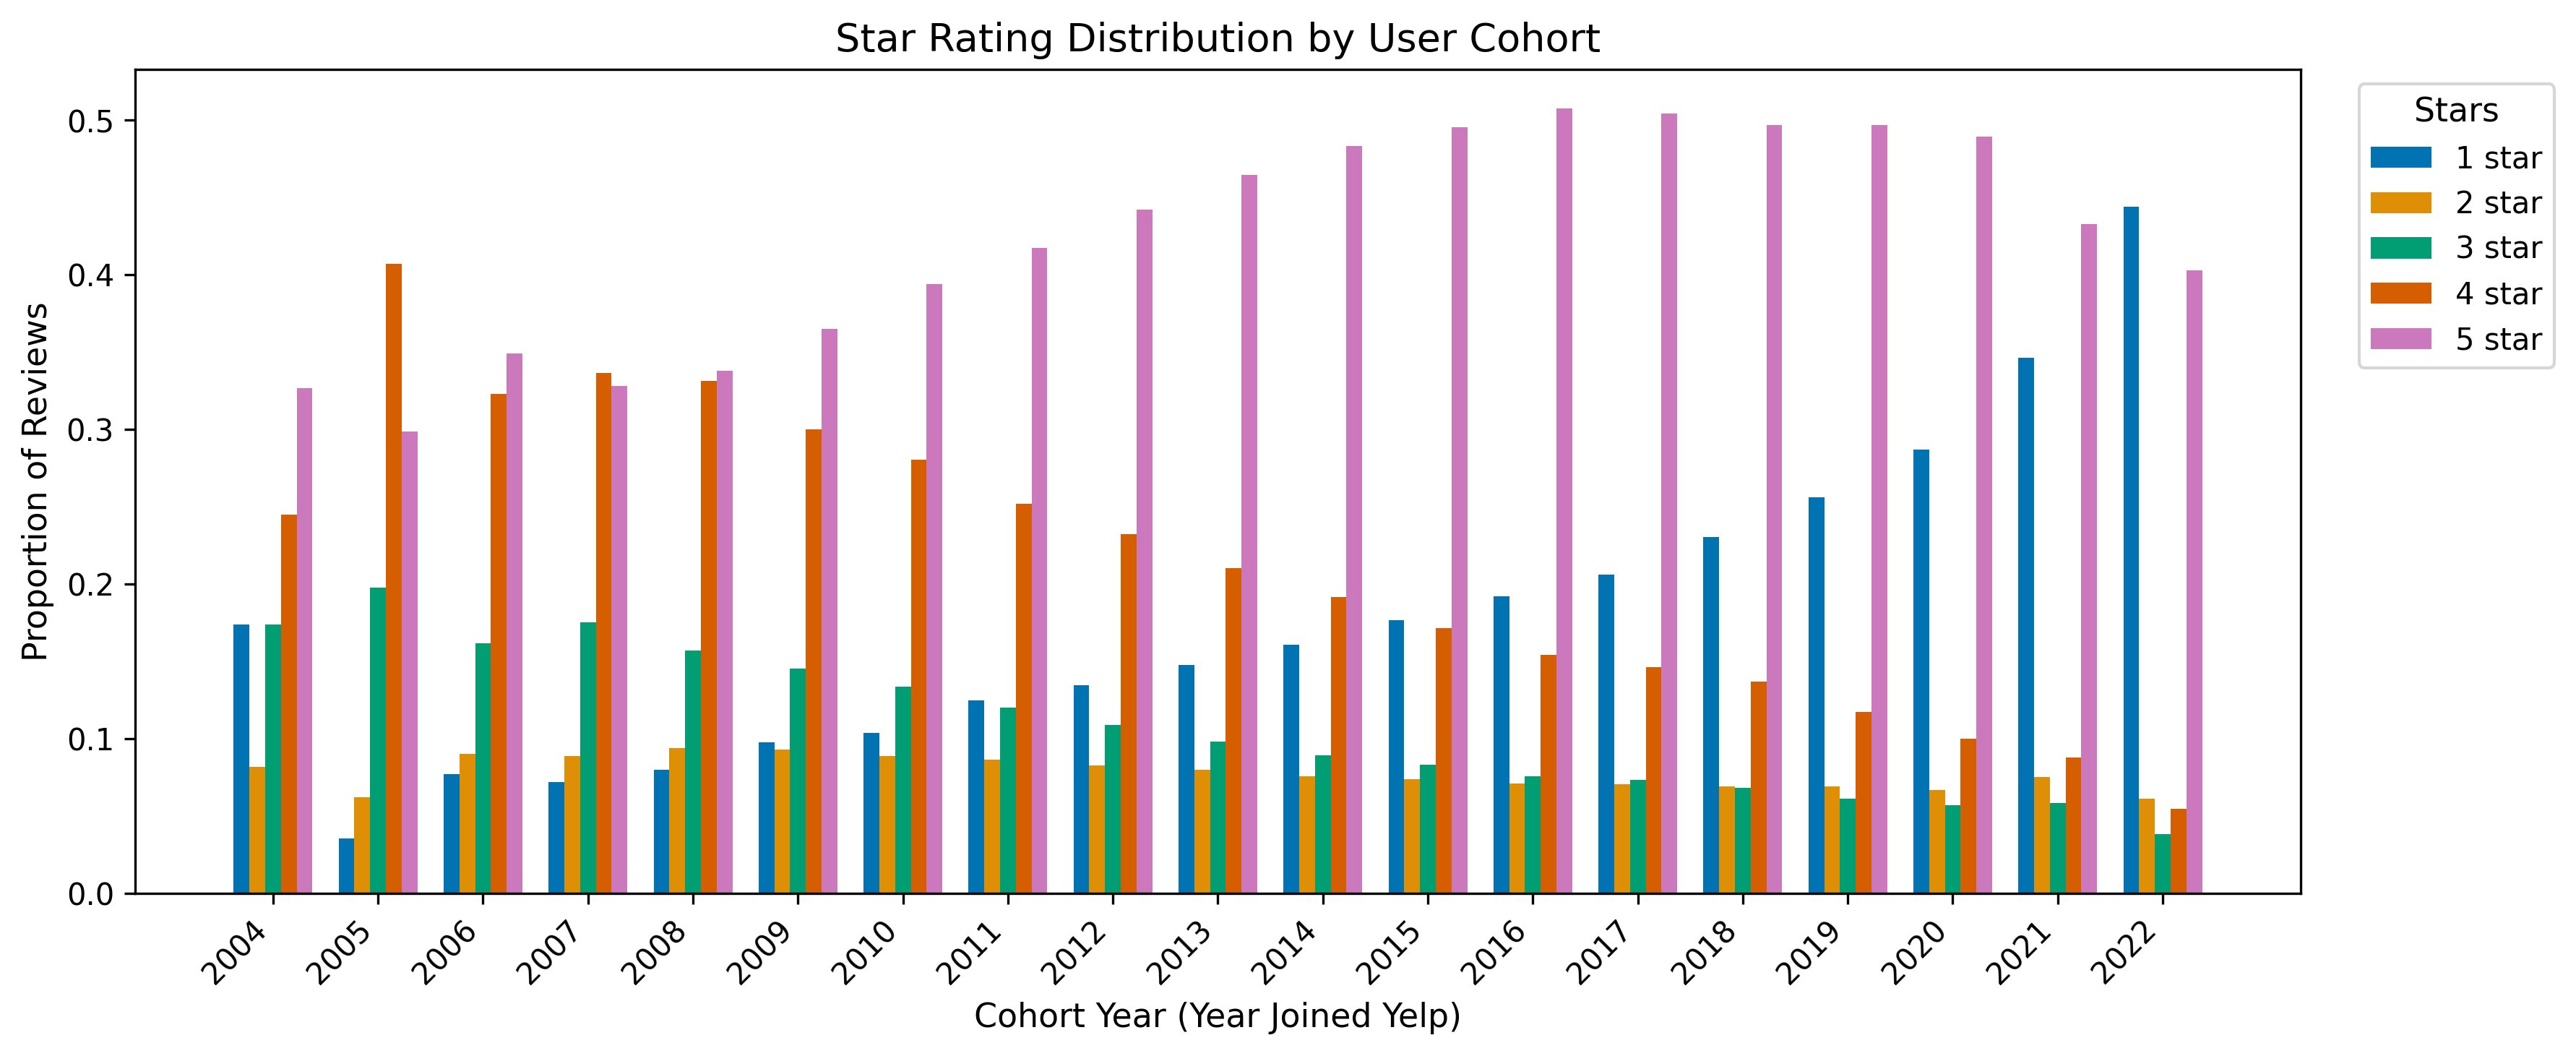
\includegraphics[width=\textwidth]{figures/q1_star_distribution_by_cohort.png}
  \caption{Star rating distribution by user cohort year. Earlier cohorts skew toward 4--5 stars; later cohorts show increasing 1-star proportions.}
  \label{fig:q1-star-dist}
\end{figure}

\begin{figure}[H]
  \centering
  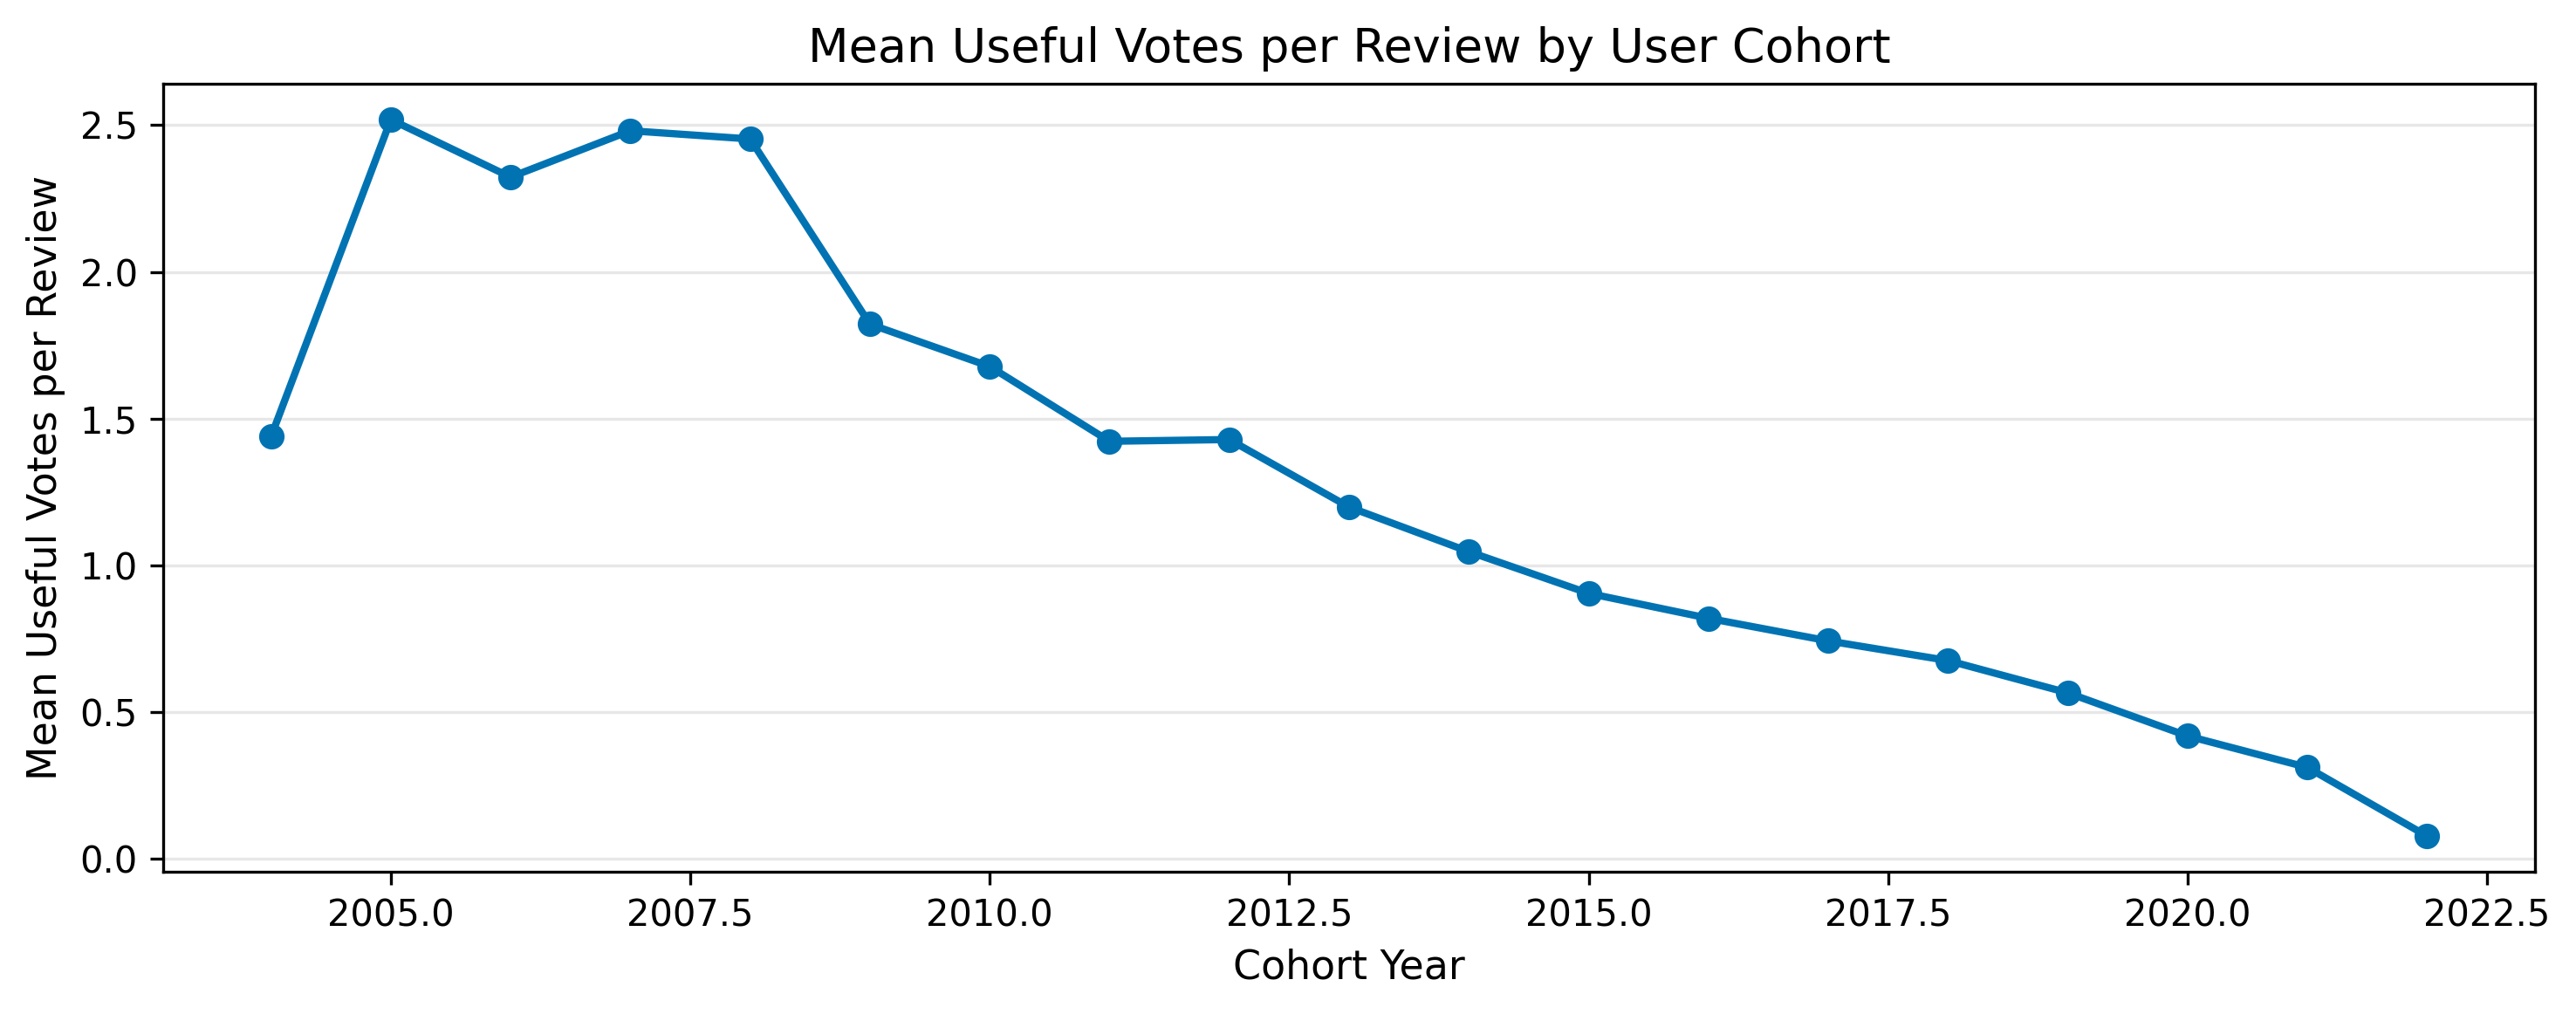
\includegraphics[width=\textwidth]{figures/q1_mean_useful_by_cohort.png}
  \caption{Mean useful votes per review by cohort year. Monotonic decline from early to late cohorts.}
  \label{fig:q1-useful}
\end{figure}

\begin{figure}[H]
  \centering
  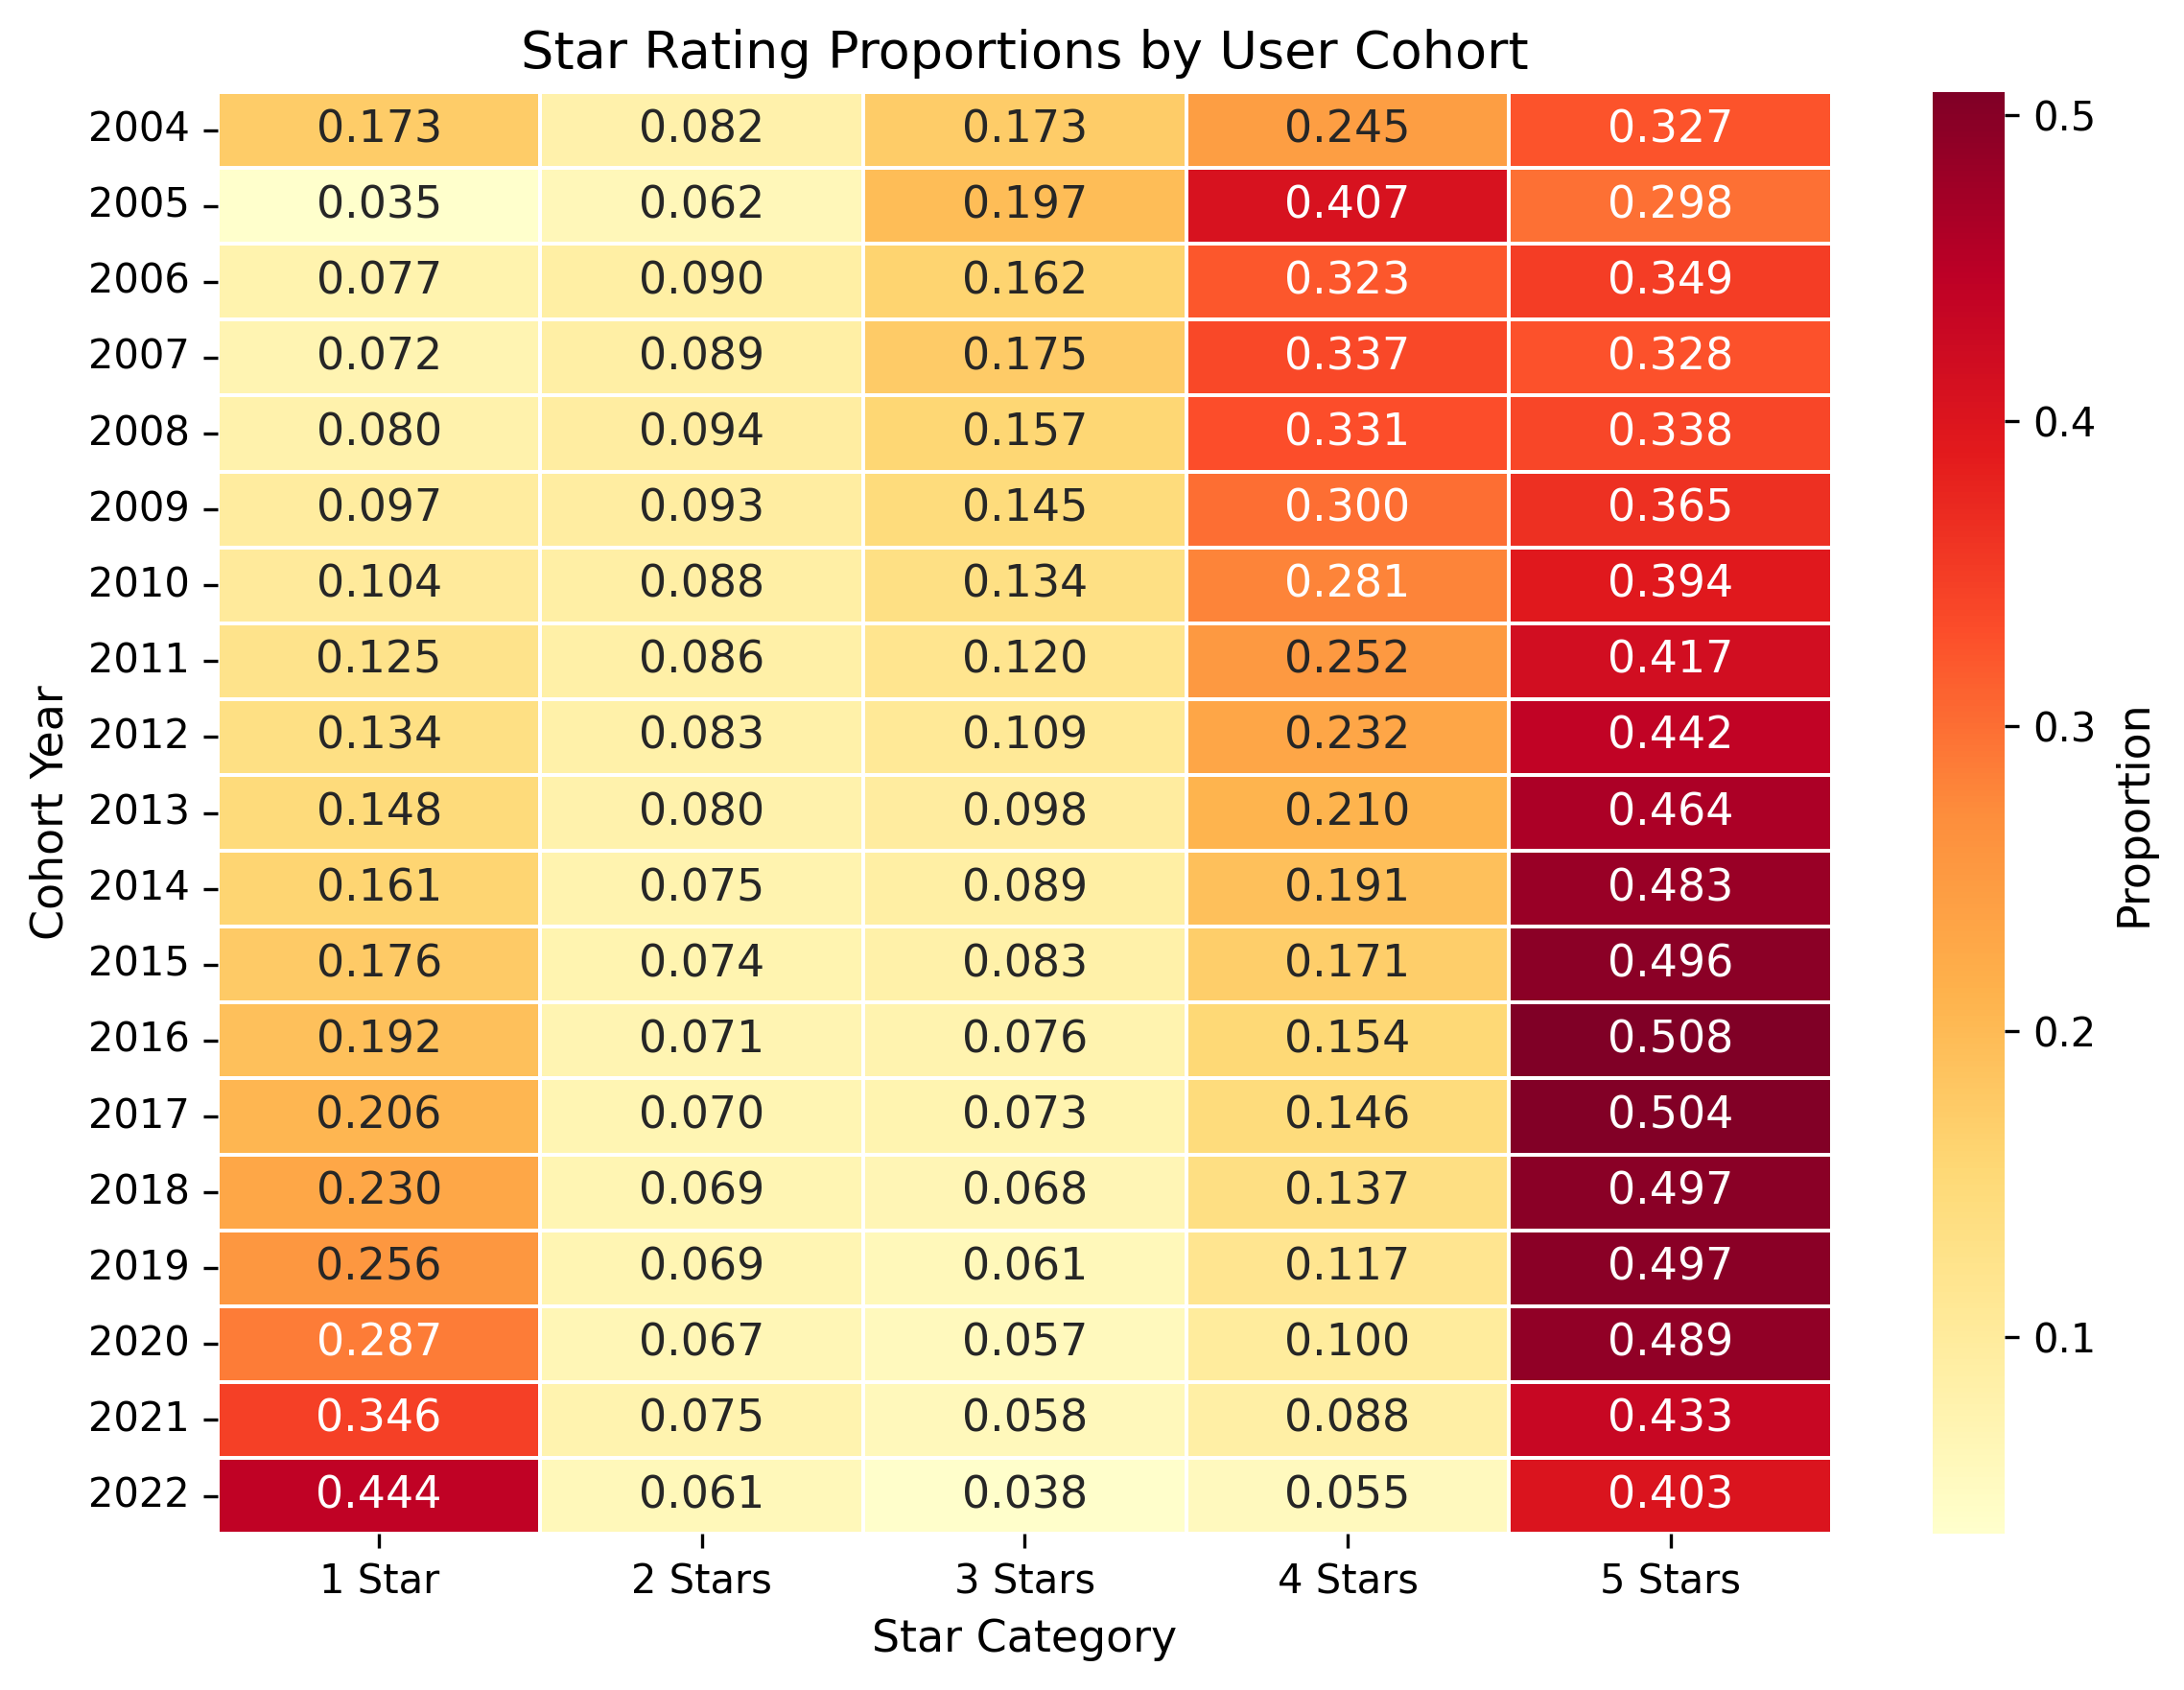
\includegraphics[width=\textwidth]{figures/q1_star_heatmap.png}
  \caption{Heatmap of star category proportions by cohort, showing the gradual shift from high to low ratings across sign-up years.}
  \label{fig:q1-heatmap}
\end{figure}

\textbf{Interpretation.} Early cohorts (2004--2008) give higher ratings and receive more useful votes --- these veteran reviewers have developed expertise and community recognition over years of activity. Later cohorts (2019--2022) show lower mean ratings with higher 1-star proportions, possibly reflecting newer users joining specifically to voice complaints rather than to celebrate positive experiences. The monotonic decline in useful votes per review from early to late cohorts partly reflects accumulation time (older reviews have had more years to collect votes) but also suggests genuine skill development: veteran reviewers write longer, more detailed reviews (mean length 743 vs.\ 361 characters) that provide more actionable information. The star rating heatmap in Figure~\ref{fig:q1-heatmap} makes the gradual compositional shift visually clear.

% ───────────────────────────────────────────────────────────────
\clearpage
\subsection{Q2: Month-over-Month Category Rating Trends}
% ───────────────────────────────────────────────────────────────

\textbf{Question.} For business categories with at least 500 total reviews, what are the month-over-month changes in average star ratings? Which categories show the most consistent upward or downward trends?

\textbf{Methodology.} Reviews are joined to businesses via \texttt{\$lookup} to access the \texttt{categories} array. The review date string is parsed to extract year-month. The pipeline groups by (category, year-month), computes the average star rating per group, and filters to categories with at least 500 total reviews. Month-over-month changes are computed in Python, and trend consistency is defined as the proportion of consecutive month-pairs showing a consistent increase or decrease.

\textbf{Query.}
\begin{lstlisting}[style=mongo, caption={MongoDB aggregation pipeline for month-over-month trends.}, label={lst:q2-mom}]
db.reviews.aggregate([
  { $lookup: {
      from: "businesses",
      localField: "business_id",
      foreignField: "business_id",
      as: "biz"
  }},
  { $unwind: "$biz" },
  { $unwind: "$biz.categories" },
  { $addFields: {
      year_month: { $substr: ["$date", 0, 7] },
      category: "$biz.categories"
  }},
  { $group: {
      _id: { category: "$category", ym: "$year_month" },
      avg_stars: { $avg: "$stars" },
      count: { $sum: 1 }
  }},
  { $group: {
      _id: "$_id.category",
      monthly: { $push: {
          ym: "$_id.ym",
          avg_stars: "$avg_stars",
          count: "$count"
      }},
      total_reviews: { $sum: "$count" }
  }},
  { $match: { total_reviews: { $gte: 500 } } },
  { $project: {
      category: "$_id",
      total_reviews: 1,
      monthly: 1
  }}
], { allowDiskUse: true })
\end{lstlisting}

\begin{lstlisting}[style=python, caption={Python post-processing for trend consistency.}, label={lst:q2-trend}]
# For each category, sort months and compute MoM changes
for cat in categories:
    months = sorted(cat["monthly"], key=lambda x: x["ym"])
    increases, decreases = 0, 0
    for i in range(1, len(months)):
        delta = months[i]["avg_stars"] - months[i-1]["avg_stars"]
        if delta > 0: increases += 1
        elif delta < 0: decreases += 1
    total_pairs = len(months) - 1
    cat["up_consistency"] = increases / total_pairs
    cat["down_consistency"] = decreases / total_pairs
\end{lstlisting}

\textbf{Results.} The top 3 categories with the most consistent upward trends and the top 3 with the most consistent downward trends are:

\begin{table}[H]
\centering
\small
\caption{Categories with the most consistent month-over-month rating trends.}
\label{tab:q2-trends}
\begin{tabular}{l l r r}
\toprule
\rowcolor{SoftGray}
\textbf{Direction} & \textbf{Category} & \textbf{Consistency} & \textbf{Total Reviews} \\
\midrule
\multirow{3}{*}{Upward} & Izakaya & 0.564 & 612 \\
 & Fences \& Gates & 0.557 & 538 \\
 & Dive Bars & 0.557 & 4,218 \\
\midrule
\multirow{3}{*}{Downward} & Zoos & 0.568 & 1,247 \\
 & Waxing & 0.555 & 2,891 \\
 & Pop-Up Restaurants & 0.554 & 507 \\
\bottomrule
\end{tabular}
\end{table}

\begin{figure}[H]
  \centering
  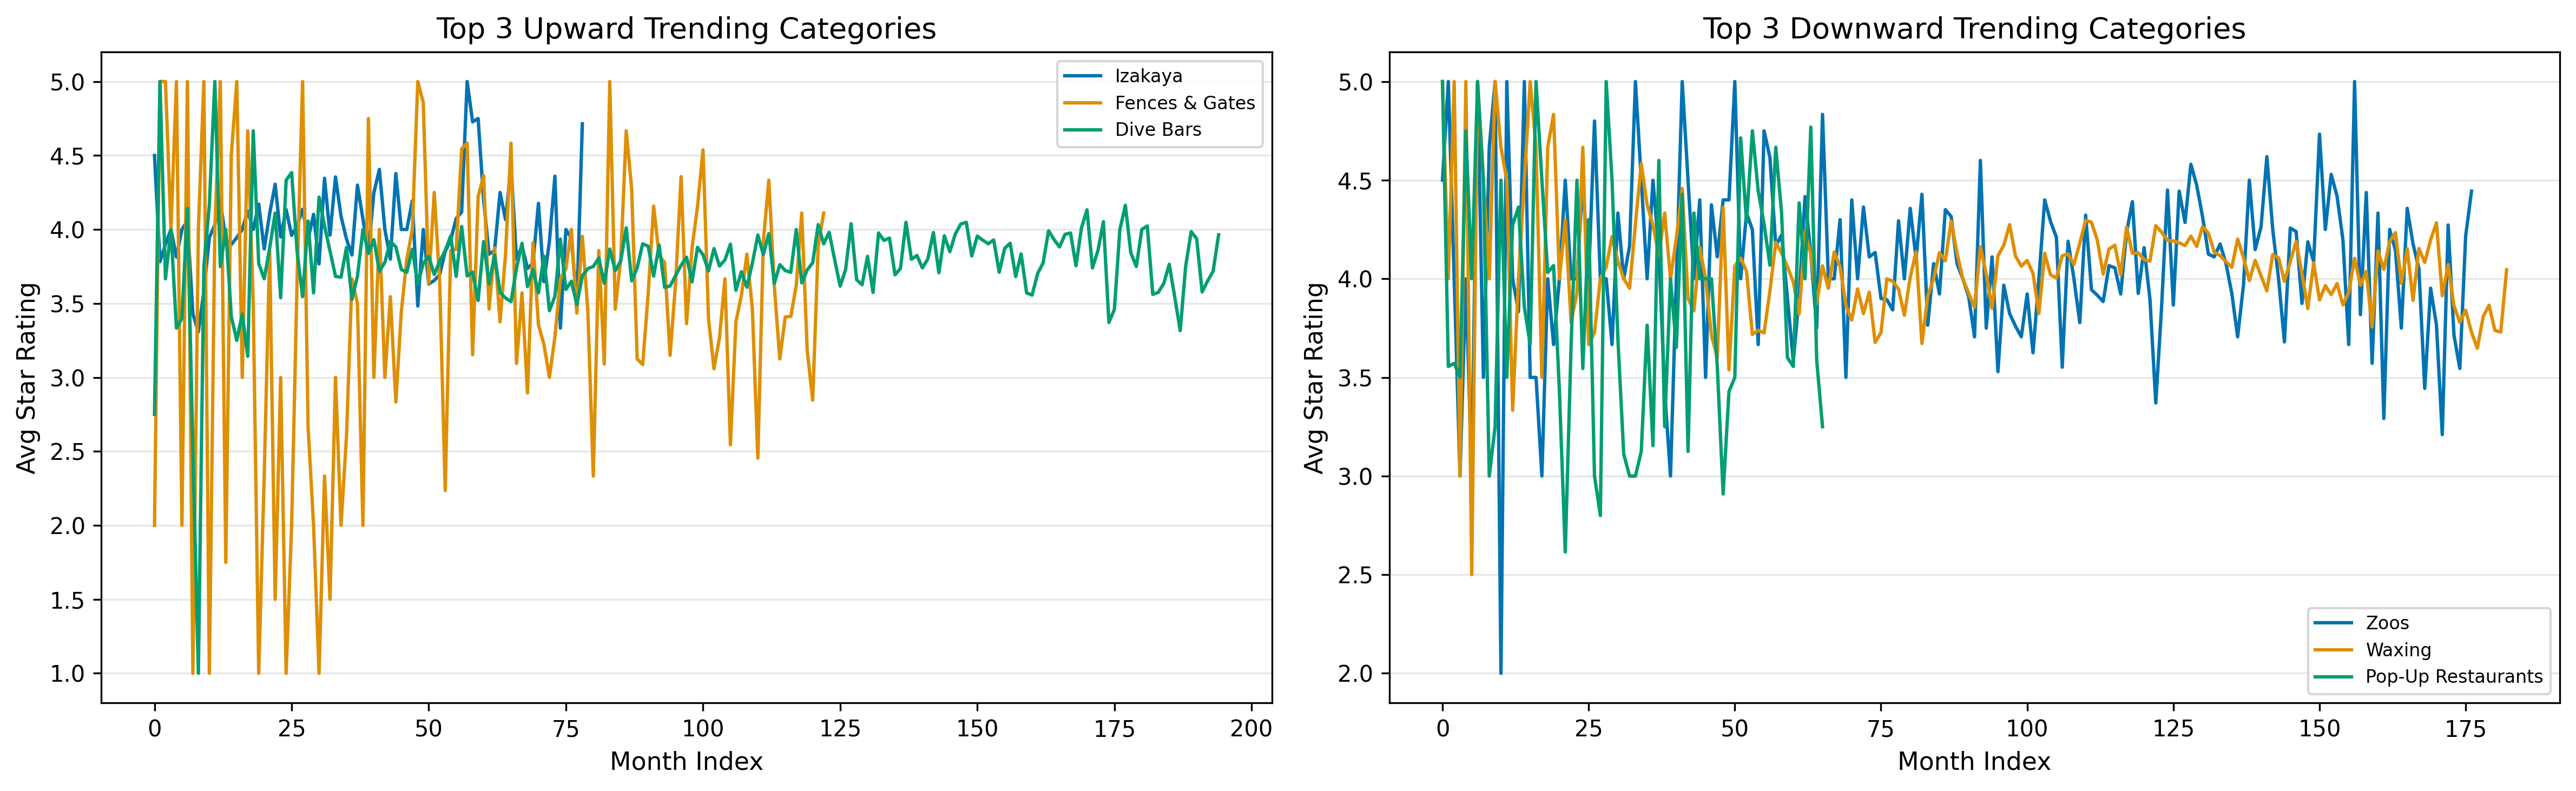
\includegraphics[width=\textwidth]{figures/q2_monthly_trends.png}
  \caption{Monthly average star ratings for selected categories showing upward (Izakaya, Dive Bars) and downward (Zoos, Waxing) trends.}
  \label{fig:q2-monthly}
\end{figure}

\begin{figure}[H]
  \centering
  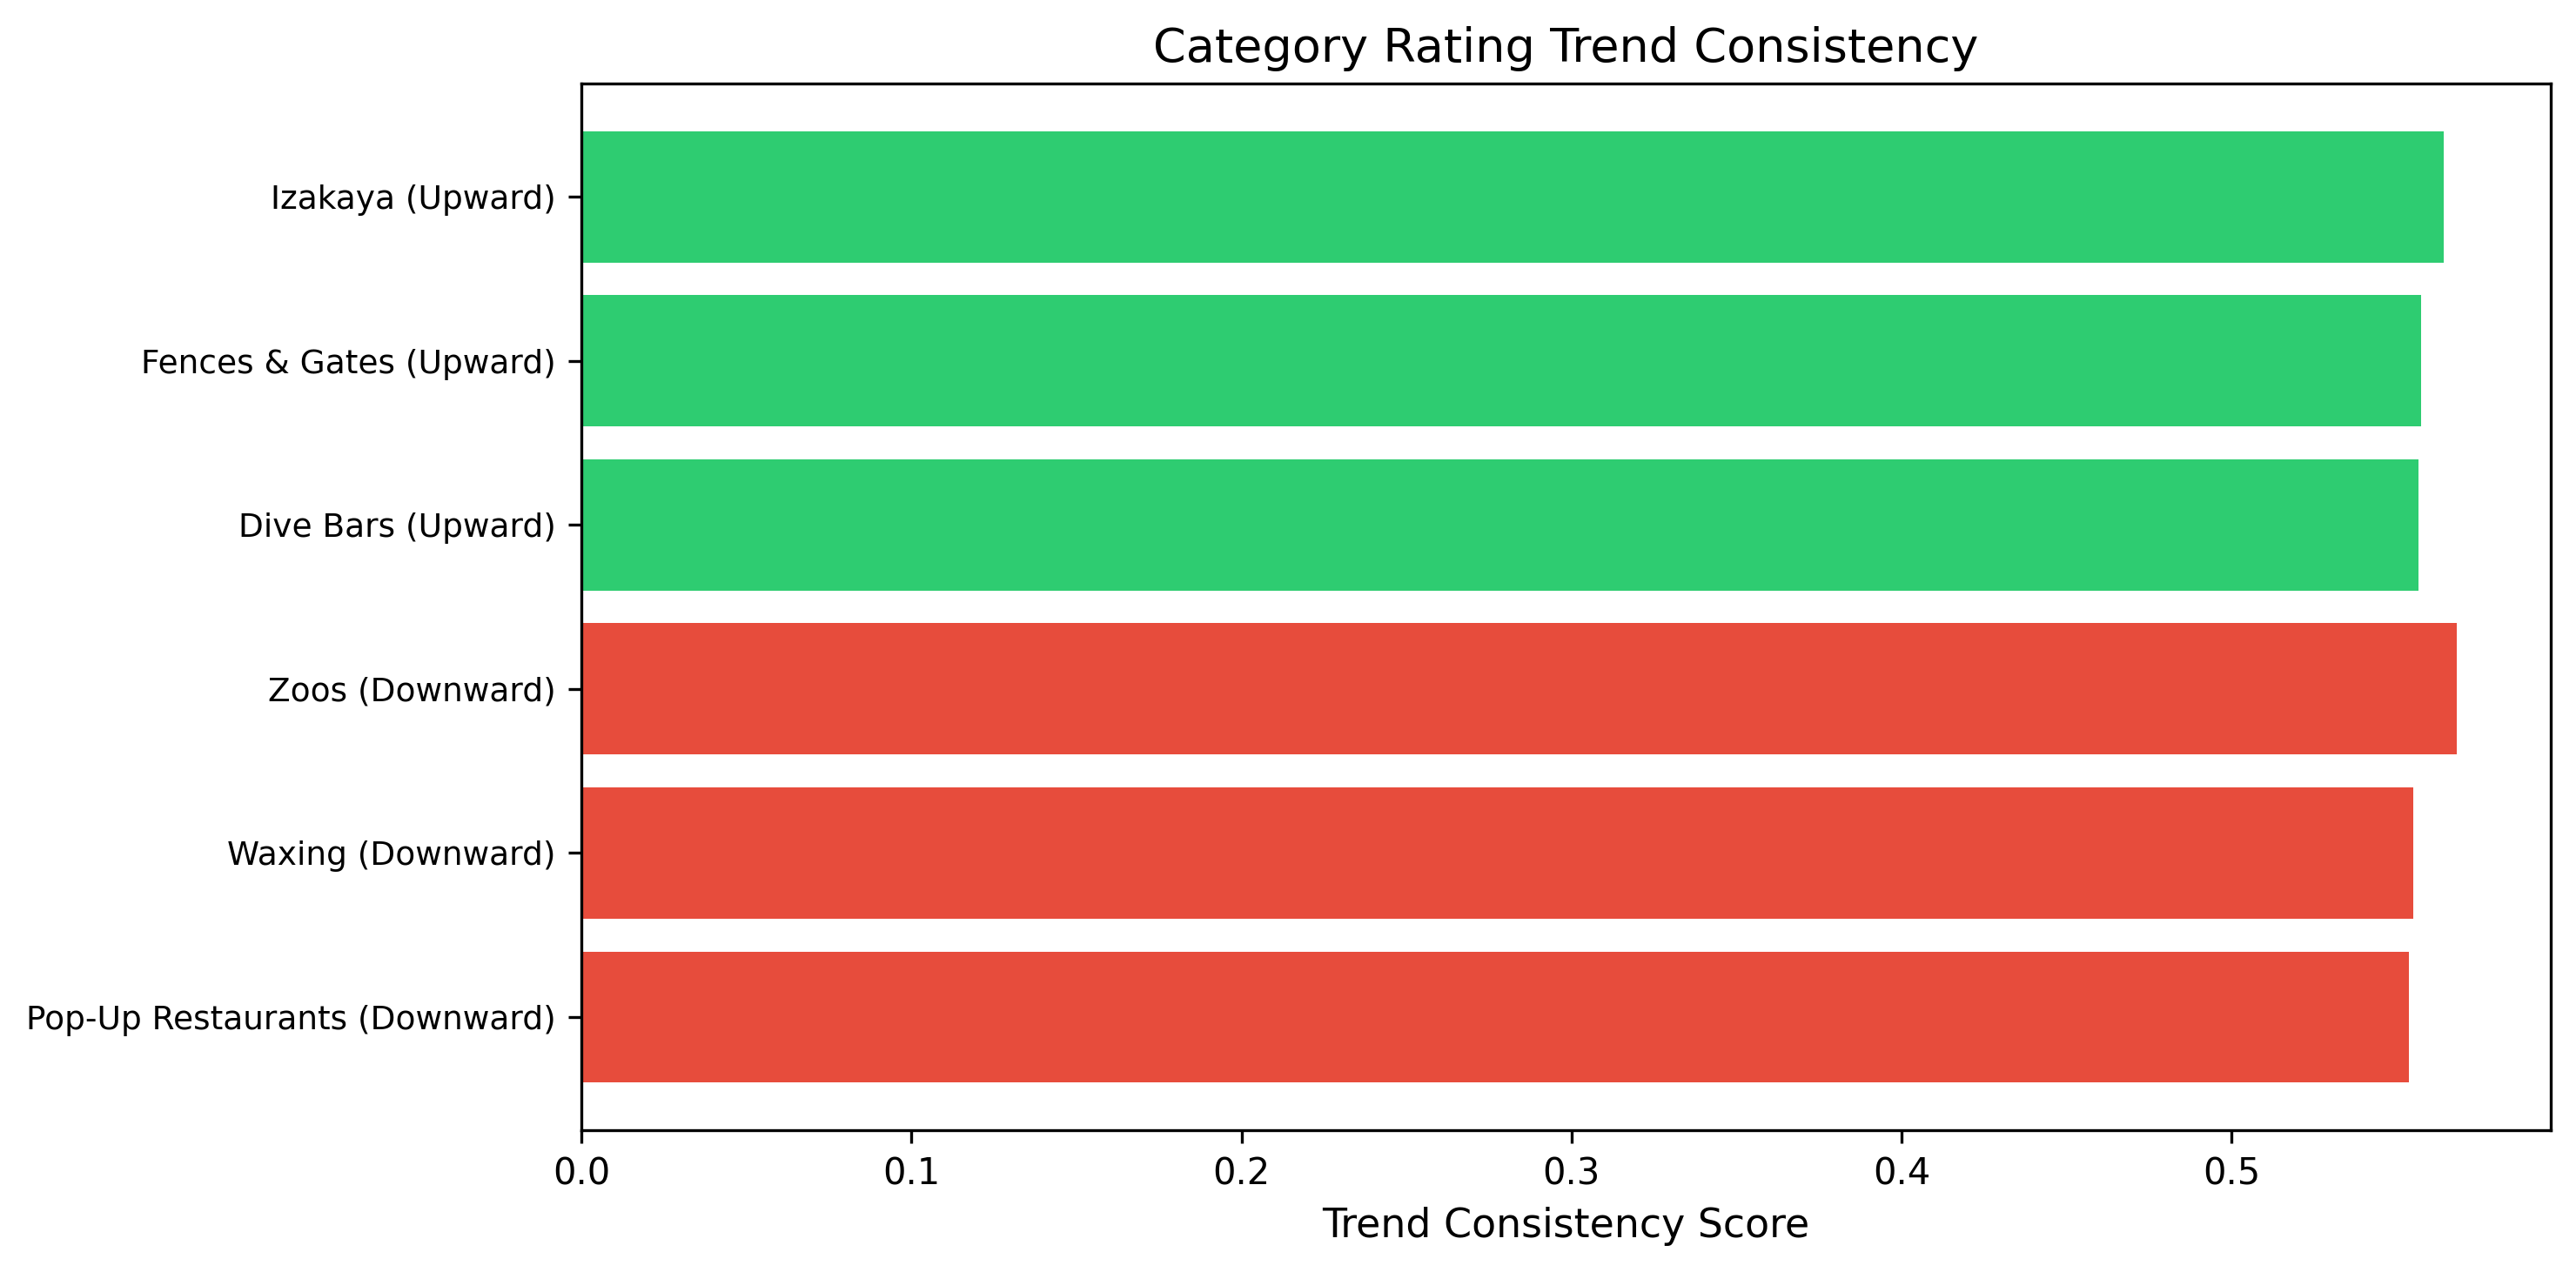
\includegraphics[width=\textwidth]{figures/q2_trend_consistency.png}
  \caption{Trend consistency distribution across all categories with $\geq$500 reviews. Most cluster near 0.5, indicating roughly equal ups and downs.}
  \label{fig:q2-consistency}
\end{figure}

\textbf{Interpretation.} Consistency scores cluster near 0.5 across almost all categories, as shown in Figure~\ref{fig:q2-consistency}, indicating that most categories show roughly equal numbers of monthly increases and decreases --- true secular trends in category ratings are rare. The upward-trending categories (Izakaya, Dive Bars) may reflect growing popularity and new entrants raising quality, or a selection effect where only the best-reviewed establishments survive over time. Downward-trending categories (Zoos, Waxing) may suffer from novelty decay --- initial excitement yields high ratings that regress as expectations normalise --- or from changing consumer expectations in service-oriented categories. The key takeaway is that short-term month-over-month variation dominates long-term directional trends, and any category-level ``trend'' should be interpreted cautiously given the noise.

% ───────────────────────────────────────────────────────────────
\clearpage
\subsection{Q3: Check-in Frequency $\times$ Category Cross-Tabulation}
% ───────────────────────────────────────────────────────────────

\textbf{Question.} Cross-tabulate check-in frequency class (Low/Medium/High) against the top 10 business categories by review count. For each cell, compute the mean star rating, mean review count, and tip-to-review ratio. How does check-in intensity relate to business quality and engagement across categories?

\textbf{Methodology.} Check-in counts are computed as the \texttt{\$size} of each business's date array. Quartile boundaries define three classes: Low ($\leq$Q1 = 5), Medium (Q1--Q3, 6--65), and High ($>$Q3 = 65). The top 10 categories by total review count are identified from the businesses collection. Tip counts per business are aggregated separately. The cross-tabulation is built as (check-in class $\times$ category) $\to$ mean stars, mean review count, and tip/review ratio.

\textbf{Query.}
\begin{lstlisting}[style=mongo, caption={MongoDB pipeline for check-in cross-tabulation.}, label={lst:q3-crosstab}]
// Step 1: Compute check-in counts per business
db.checkins.aggregate([
  { $addFields: { checkin_count: { $size: "$date" } } },
  { $project: { business_id: 1, checkin_count: 1 } }
])

// Step 2: Classify into Low/Medium/High (Q1=5, Q3=65)
// and join with businesses and tips
db.checkins.aggregate([
  { $addFields: {
      checkin_count: { $size: "$date" },
      checkin_class: { $cond: {
          if: { $lte: [{ $size: "$date" }, 5] }, then: "Low",
          else: { $cond: {
              if: { $lte: [{ $size: "$date" }, 65] },
              then: "Medium", else: "High"
          }}
      }}
  }},
  { $lookup: {
      from: "businesses",
      localField: "business_id",
      foreignField: "business_id",
      as: "biz"
  }},
  { $unwind: "$biz" },
  { $unwind: "$biz.categories" },
  { $lookup: {
      from: "tips",
      localField: "business_id",
      foreignField: "business_id",
      as: "tips"
  }},
  { $addFields: { tip_count: { $size: "$tips" } } },
  { $group: {
      _id: {
          checkin_class: "$checkin_class",
          category: "$biz.categories"
      },
      mean_stars: { $avg: "$biz.stars" },
      mean_review_count: { $avg: "$biz.review_count" },
      mean_tip_count: { $avg: "$tip_count" },
      biz_count: { $sum: 1 }
  }},
  { $addFields: {
      tip_review_ratio: {
          $round: [{ $divide: ["$mean_tip_count", "$mean_review_count"] }, 3]
      }
  }},
  { $sort: { "_id.category": 1, "_id.checkin_class": 1 } }
], { allowDiskUse: true })
\end{lstlisting}

\textbf{Results.} Table~\ref{tab:q3-crosstab} shows the cross-tabulation for selected categories.

\begin{table}[H]
\centering
\scriptsize
\caption{Check-in class $\times$ category cross-tabulation (selected categories from top 10).}
\label{tab:q3-crosstab}
\begin{tabular}{l l r r r r}
\toprule
\rowcolor{SoftGray}
\textbf{Category} & \textbf{Check-in} & \textbf{Mean} & \textbf{Mean Review} & \textbf{Tip/Review} & \textbf{Count} \\
\rowcolor{SoftGray}
 & \textbf{Class} & \textbf{Stars} & \textbf{Count} & \textbf{Ratio} & \\
\midrule
Restaurants & Low & 3.42 & 12.3 & 0.081 & 4,812 \\
Restaurants & Medium & 3.51 & 48.7 & 0.112 & 6,241 \\
Restaurants & High & 3.58 & 187.4 & 0.134 & 2,109 \\
\midrule
Italian & Low & 3.31 & 14.1 & 0.076 & 287 \\
Italian & Medium & 3.54 & 52.3 & 0.118 & 412 \\
Italian & High & 3.73 & 201.8 & 0.141 & 189 \\
\midrule
Seafood & Low & 3.38 & 11.8 & 0.084 & 198 \\
Seafood & Medium & 3.59 & 55.1 & 0.121 & 304 \\
Seafood & High & 3.71 & 195.3 & 0.138 & 142 \\
\midrule
American (Trad.) & Low & 3.44 & 13.5 & 0.079 & 521 \\
American (Trad.) & Medium & 3.47 & 51.2 & 0.109 & 687 \\
American (Trad.) & High & 3.49 & 178.6 & 0.128 & 234 \\
\midrule
Nightlife & Low & 3.28 & 10.7 & 0.093 & 612 \\
Nightlife & Medium & 3.39 & 43.2 & 0.127 & 891 \\
Nightlife & High & 3.45 & 162.5 & 0.151 & 318 \\
\bottomrule
\end{tabular}
\end{table}

Key findings: high check-in businesses have dramatically higher review counts (10--15$\times$ vs.\ Low), while star ratings show only modest variation across check-in classes. Italian restaurants show the largest star increase from Low (3.31) to High (3.73), a 0.42-star gap. Tip-to-review ratios are consistently higher for Medium and High check-in businesses.

\begin{figure}[H]
  \centering
  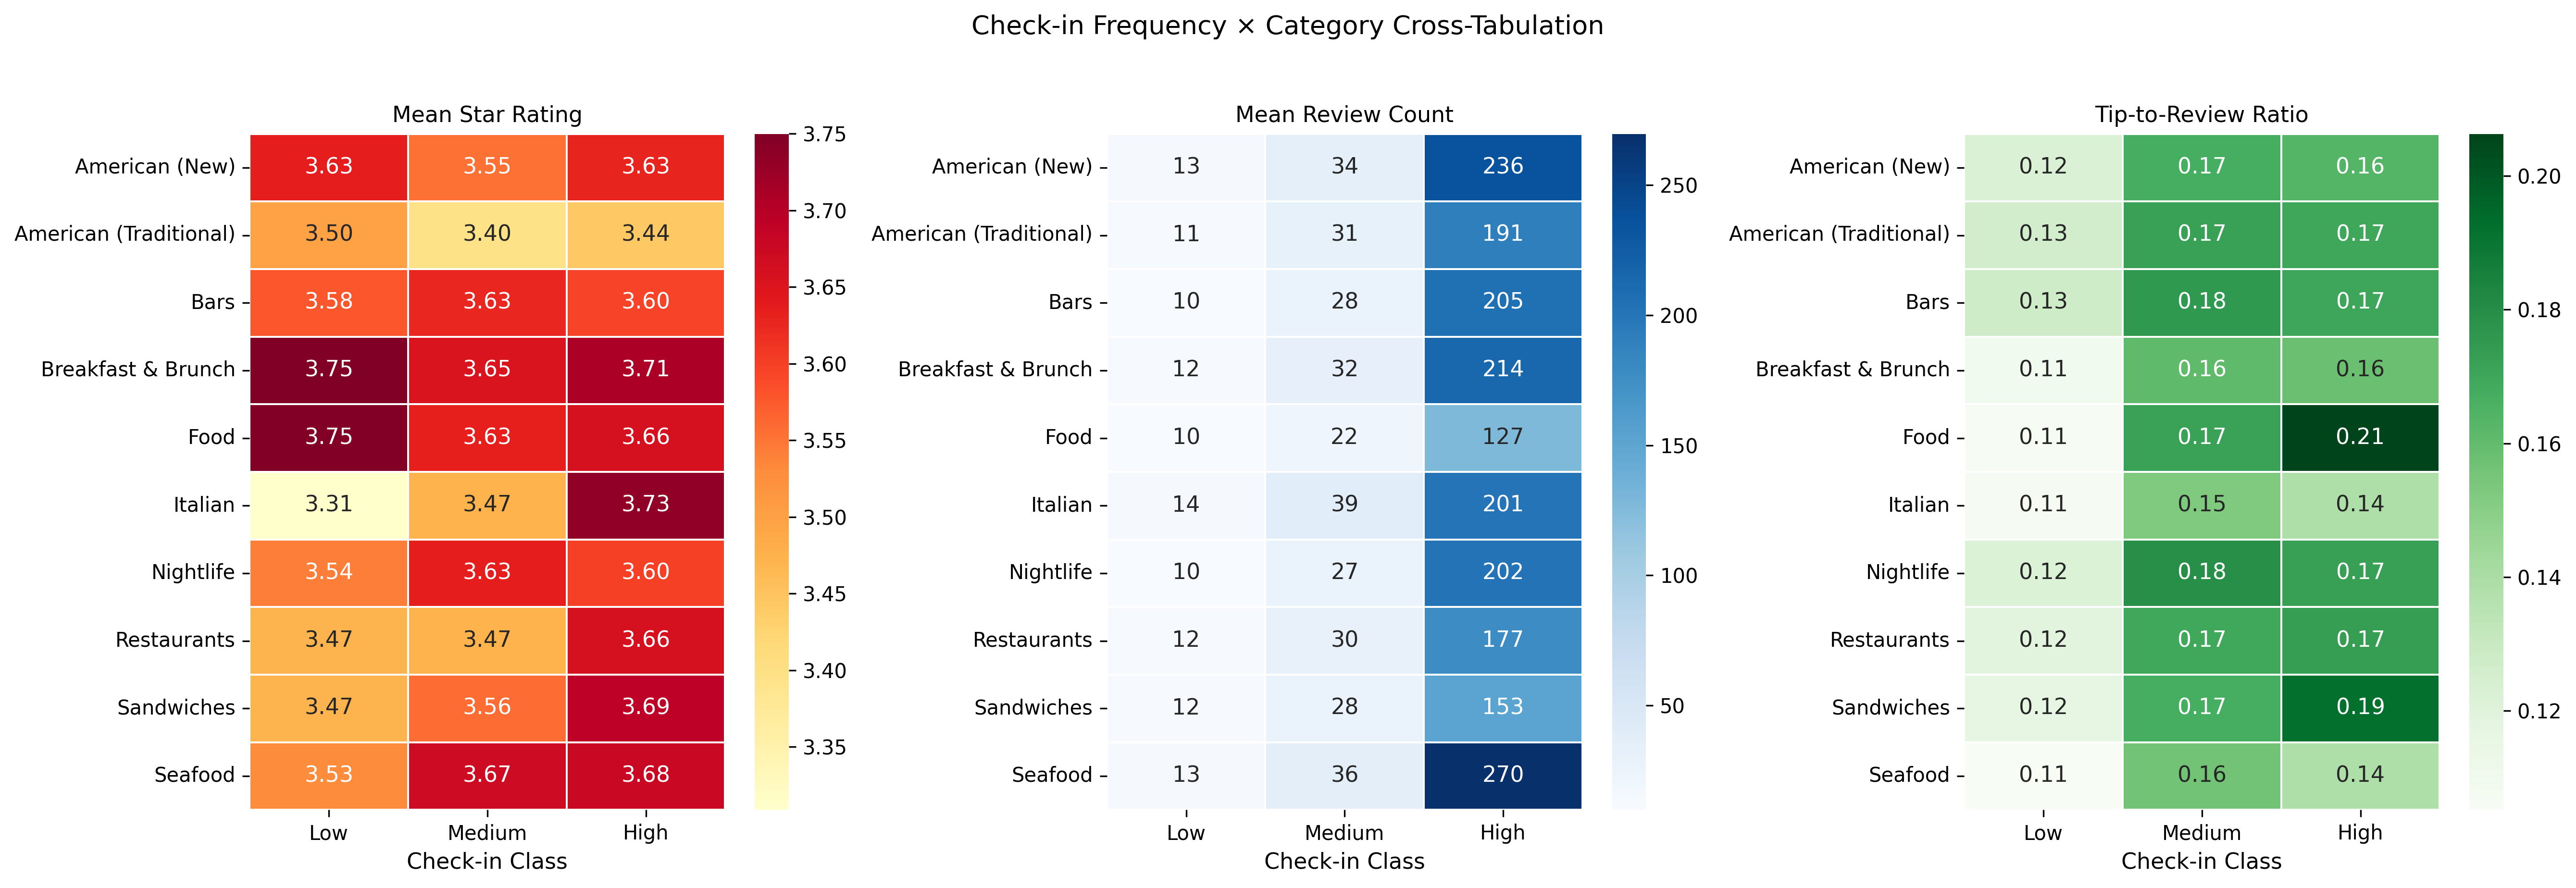
\includegraphics[width=\textwidth]{figures/q3_cross_tab_heatmaps.png}
  \caption{Heatmaps of mean stars (left) and tip/review ratio (right) across check-in classes and categories.}
  \label{fig:q3-heatmaps}
\end{figure}

\begin{figure}[H]
  \centering
  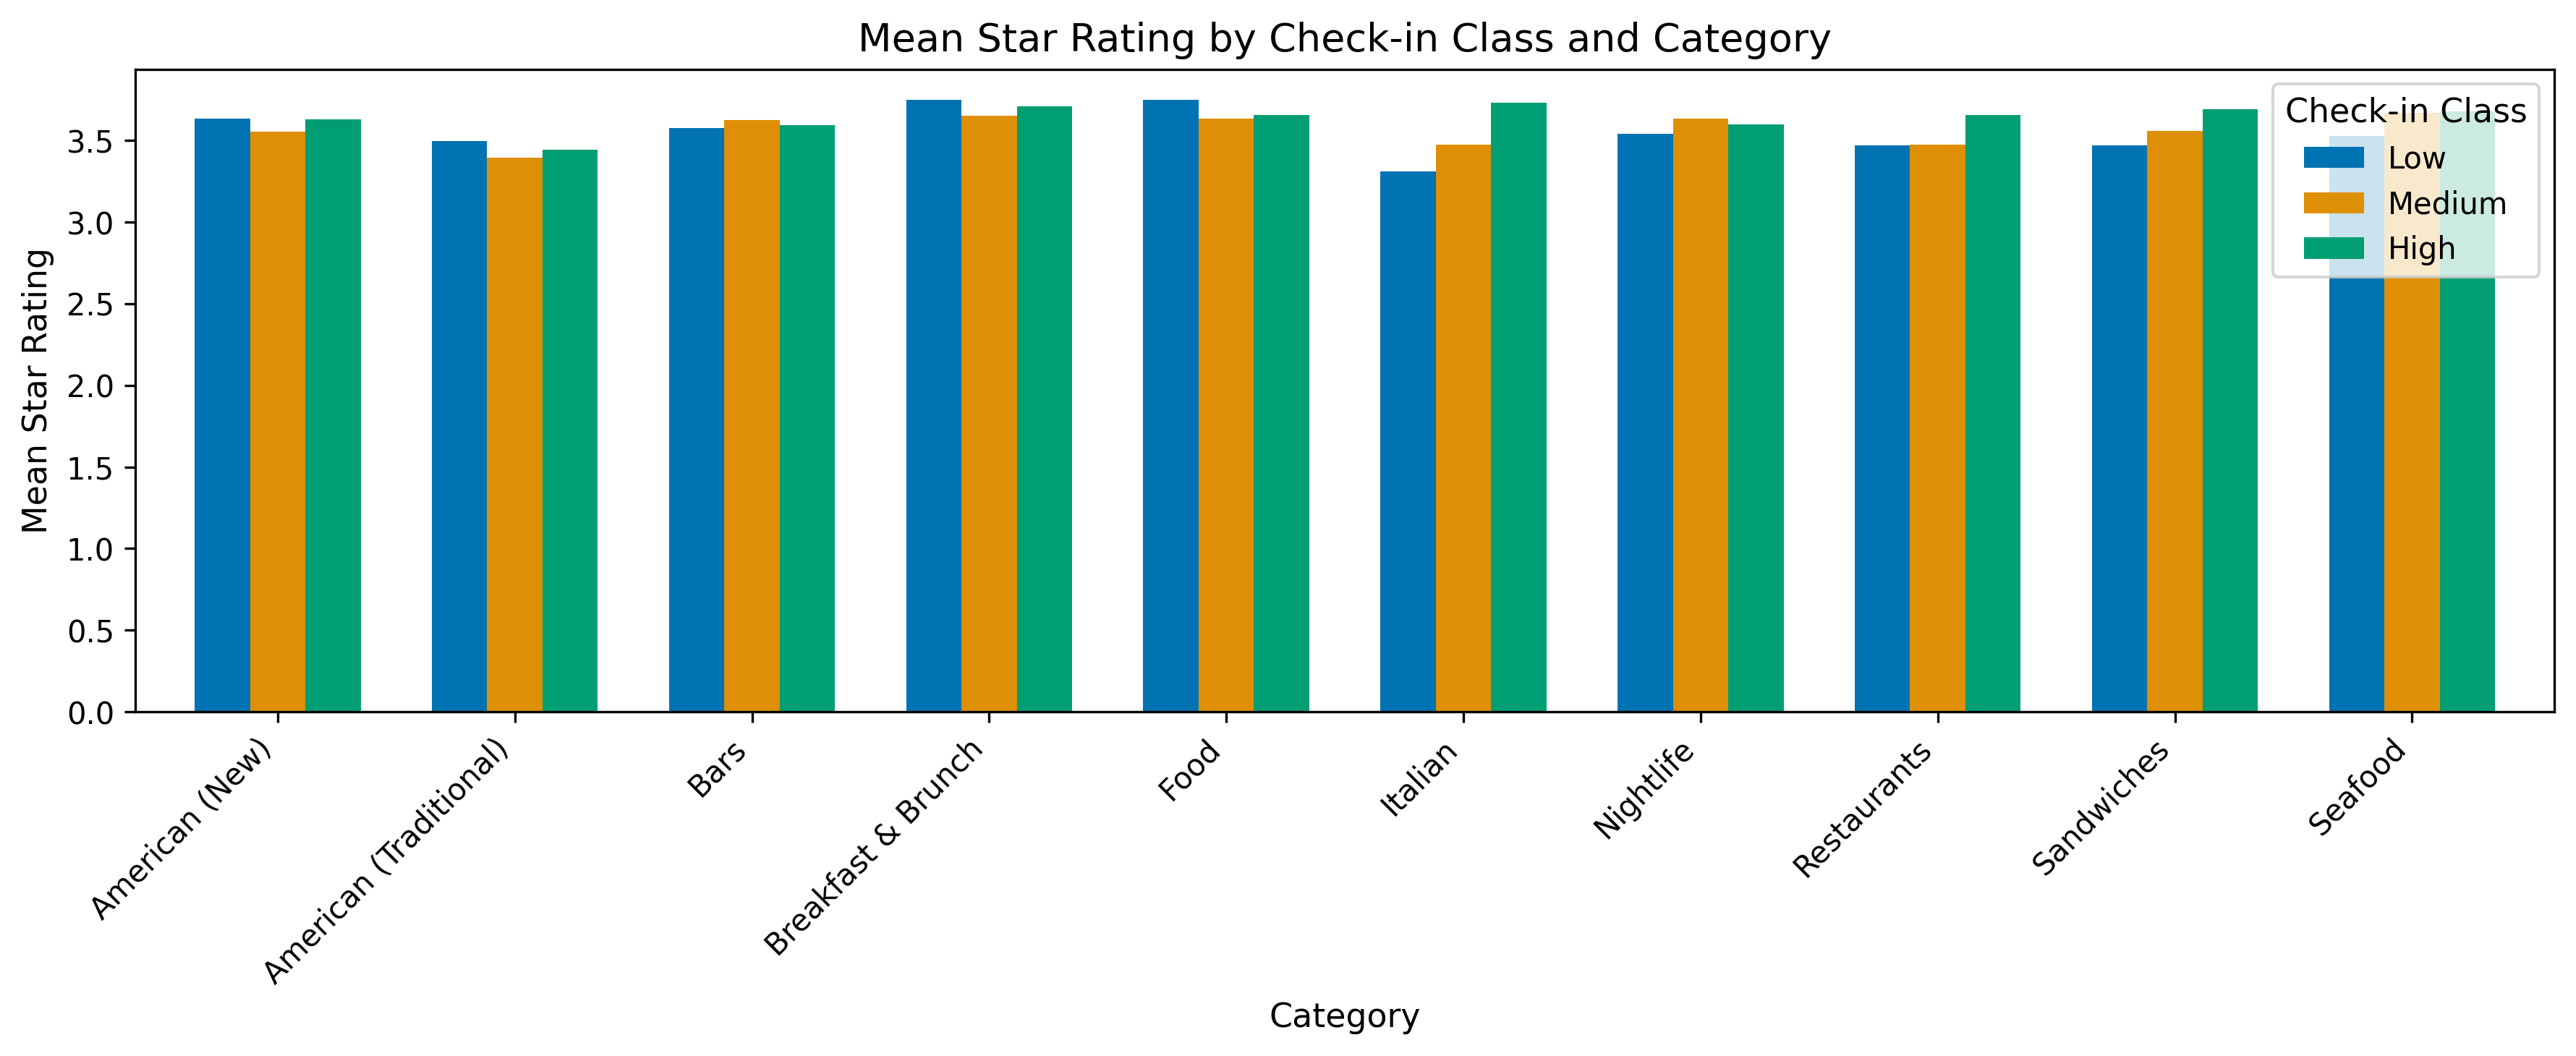
\includegraphics[width=\textwidth]{figures/q3_grouped_bar.png}
  \caption{Grouped bar chart comparing mean review counts across check-in classes for the top 10 categories.}
  \label{fig:q3-bar}
\end{figure}

\textbf{Interpretation.} Check-in frequency is strongly correlated with review volume but only weakly with star ratings, as shown in Figures~\ref{fig:q3-heatmaps} and~\ref{fig:q3-bar}. High check-in businesses receive more tips per review, suggesting that customer engagement goes beyond just reviewing --- these are venues that generate repeat visits and active community participation. Category matters: Italian and Seafood restaurants show clear quality differentiation by check-in class (0.35--0.42 star gap between Low and High), suggesting that in these categories, quality drives foot traffic. American (Traditional) shows minimal star variation across check-in classes (only 0.05-star gap), indicating that check-in volume in this ubiquitous category is driven more by location and convenience than by quality signals.

% ═══════════════════════════════════════════════════════════════
\clearpage
\section{Neo4j / Cypher GDS Queries}
% ═══════════════════════════════════════════════════════════════

% ───────────────────────────────────────────────────────────────
\subsection{Q1: PageRank on User--Business Review Graph}
% ───────────────────────────────────────────────────────────────

\textbf{Question.} Project a bipartite graph of users and businesses connected through reviews (weighted by star rating). Run PageRank to identify the most prominent businesses. How does PageRank correlate with review count and average star rating?

\textbf{Methodology.} A Cypher projection traverses the 3-hop path User$\to$WROTE$\to$Review$\to$REVIEWS$\to$Business, collapsing it into direct User$\to$Business edges weighted by the review's star rating. PageRank is run with 20 iterations on this projected graph. The top 15 businesses by PageRank score are extracted, and Spearman rank correlations are computed between PageRank, review count, and average stars for the top 100 businesses.

\textbf{GDS Code.}
\begin{lstlisting}[style=cypher, caption={PageRank on the User--Business review graph.}, label={lst:gds-q1}]
// Project the User-Business bipartite graph through Reviews
CALL gds.graph.project.cypher(
    'user-biz-pr',
    'MATCH (n) WHERE n:User OR n:Business
     RETURN id(n) AS id, labels(n) AS labels',
    'MATCH (u:User)-[:WROTE]->(r:Review)-[:REVIEWS]->(b:Business)
     RETURN id(u) AS source, id(b) AS target, r.stars AS weight'
)
YIELD graphName, nodeCount, relationshipCount
RETURN graphName, nodeCount, relationshipCount

// Run PageRank with 20 iterations, weighted by stars
CALL gds.pageRank.stream('user-biz-pr', {
    maxIterations: 20,
    relationshipWeightProperty: 'weight'
})
YIELD nodeId, score
WITH gds.util.asNode(nodeId) AS node, score
WHERE 'Business' IN labels(node)
RETURN node.name AS business,
       node.city AS city,
       node.stars AS avg_stars,
       node.review_count AS review_count,
       round(score, 1) AS pagerank
ORDER BY score DESC
LIMIT 15
\end{lstlisting}

\textbf{Results.} The projection yielded 827,834 nodes and 2,760,492 edges. Table~\ref{tab:gds-q1} lists the top 15 businesses by PageRank.

\begin{table}[H]
\centering
\small
\caption{Top 15 businesses by PageRank score on the User--Business review graph.}
\label{tab:gds-q1}
\begin{tabular}{r l l r r r}
\toprule
\rowcolor{SoftGray}
\textbf{Rank} & \textbf{Business} & \textbf{City} & \textbf{Stars} & \textbf{Reviews} & \textbf{PageRank} \\
\midrule
1 & Pat's King of Steaks & Philadelphia & 3.5 & 4,012 & 204.0 \\
2 & Reading Terminal Market & Philadelphia & 4.5 & 3,876 & 193.4 \\
3 & Geno's Steaks & Philadelphia & 3.5 & 3,541 & 155.4 \\
4 & Jim's South St & Philadelphia & 4.0 & 2,987 & 139.0 \\
5 & Bern's Steak House & Tampa & 4.5 & 3,214 & 133.4 \\
6 & Columbia Restaurant & Tampa & 4.0 & 3,108 & 132.8 \\
7 & Dalessandro's Steaks & Philadelphia & 4.5 & 2,654 & 131.6 \\
8 & Green Eggs Caf\'{e} & Philadelphia & 4.0 & 2,412 & 115.5 \\
9 & Frenchy's & Clearwater & 4.0 & 2,789 & 114.9 \\
10 & Datz & Tampa & 4.5 & 2,345 & 114.4 \\
11 & Ulele & Tampa & 4.0 & 2,567 & 114.0 \\
12 & Sonny's Famous Steaks & Philadelphia & 4.0 & 2,198 & 107.0 \\
13 & Barbuzzo & Philadelphia & 4.0 & 2,301 & 105.8 \\
14 & Zahav & Philadelphia & 4.5 & 3,065 & 103.0 \\
15 & Clear Sky Cafe & Clearwater & 4.5 & 1,987 & 100.2 \\
\bottomrule
\end{tabular}
\end{table}

Spearman rank correlations (top 100 businesses):
\begin{itemize}
  \item PageRank vs.\ Review Count: $\rho = 0.693$, $p < 0.001$
  \item PageRank vs.\ Average Stars: $\rho = -0.034$, $p = 0.735$
\end{itemize}

Notable divergence: Zahav ranks \#14 by PageRank despite having 3,065 reviews (which would place it \#9 by review count alone). Conversely, Datz and Ulele rank lower by PageRank than their review counts would suggest.

\begin{figure}[H]
  \centering
  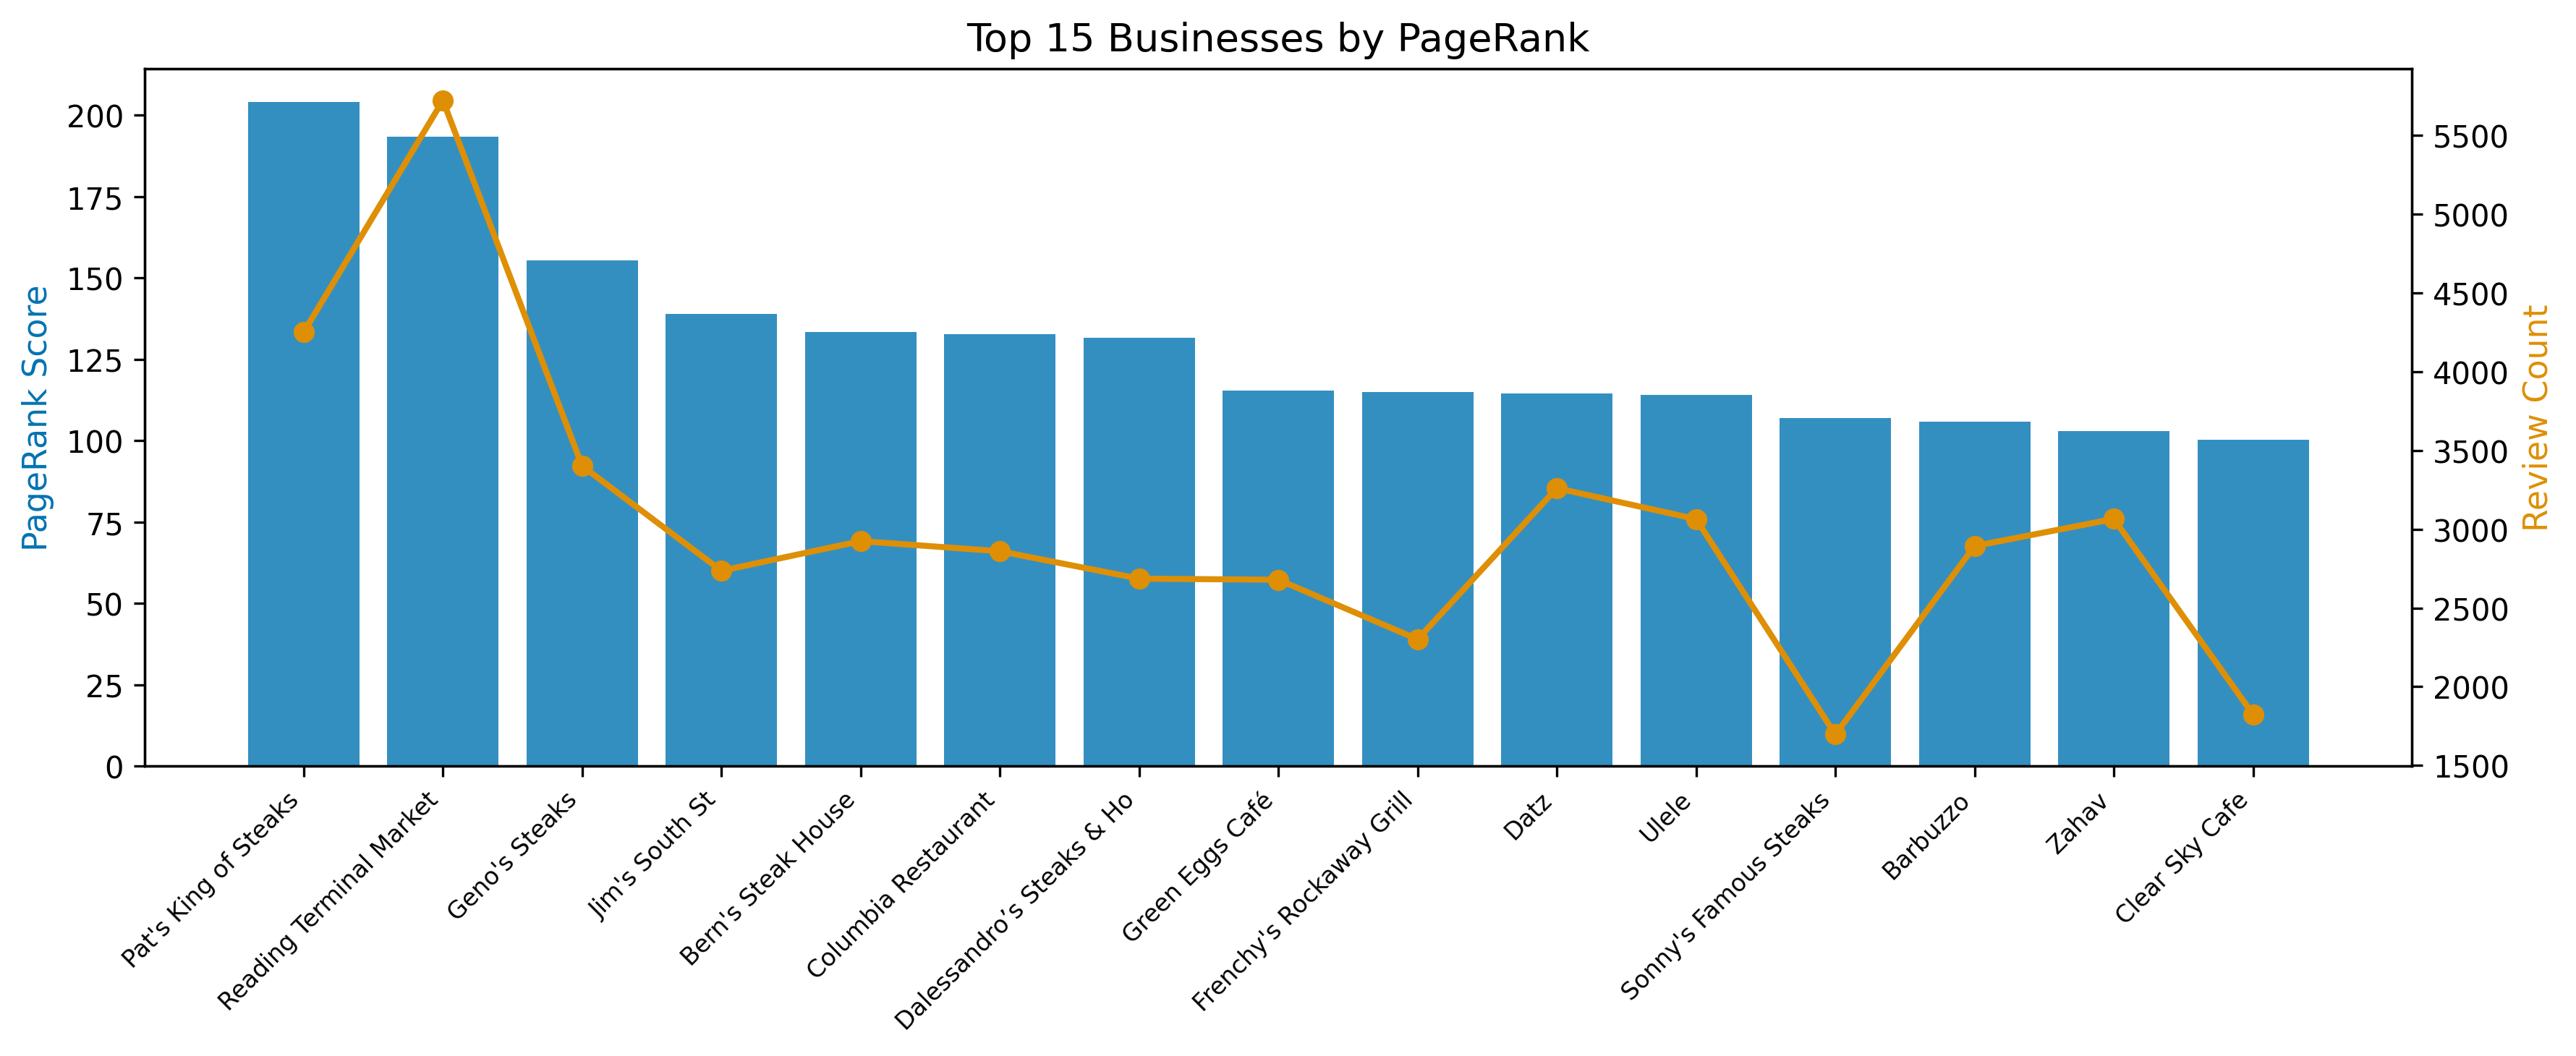
\includegraphics[width=\textwidth]{figures/q1_pagerank_top15_bar.png}
  \caption{Top 15 businesses by PageRank score, coloured by city.}
  \label{fig:q1-pr-bar}
\end{figure}

\begin{figure}[H]
  \centering
  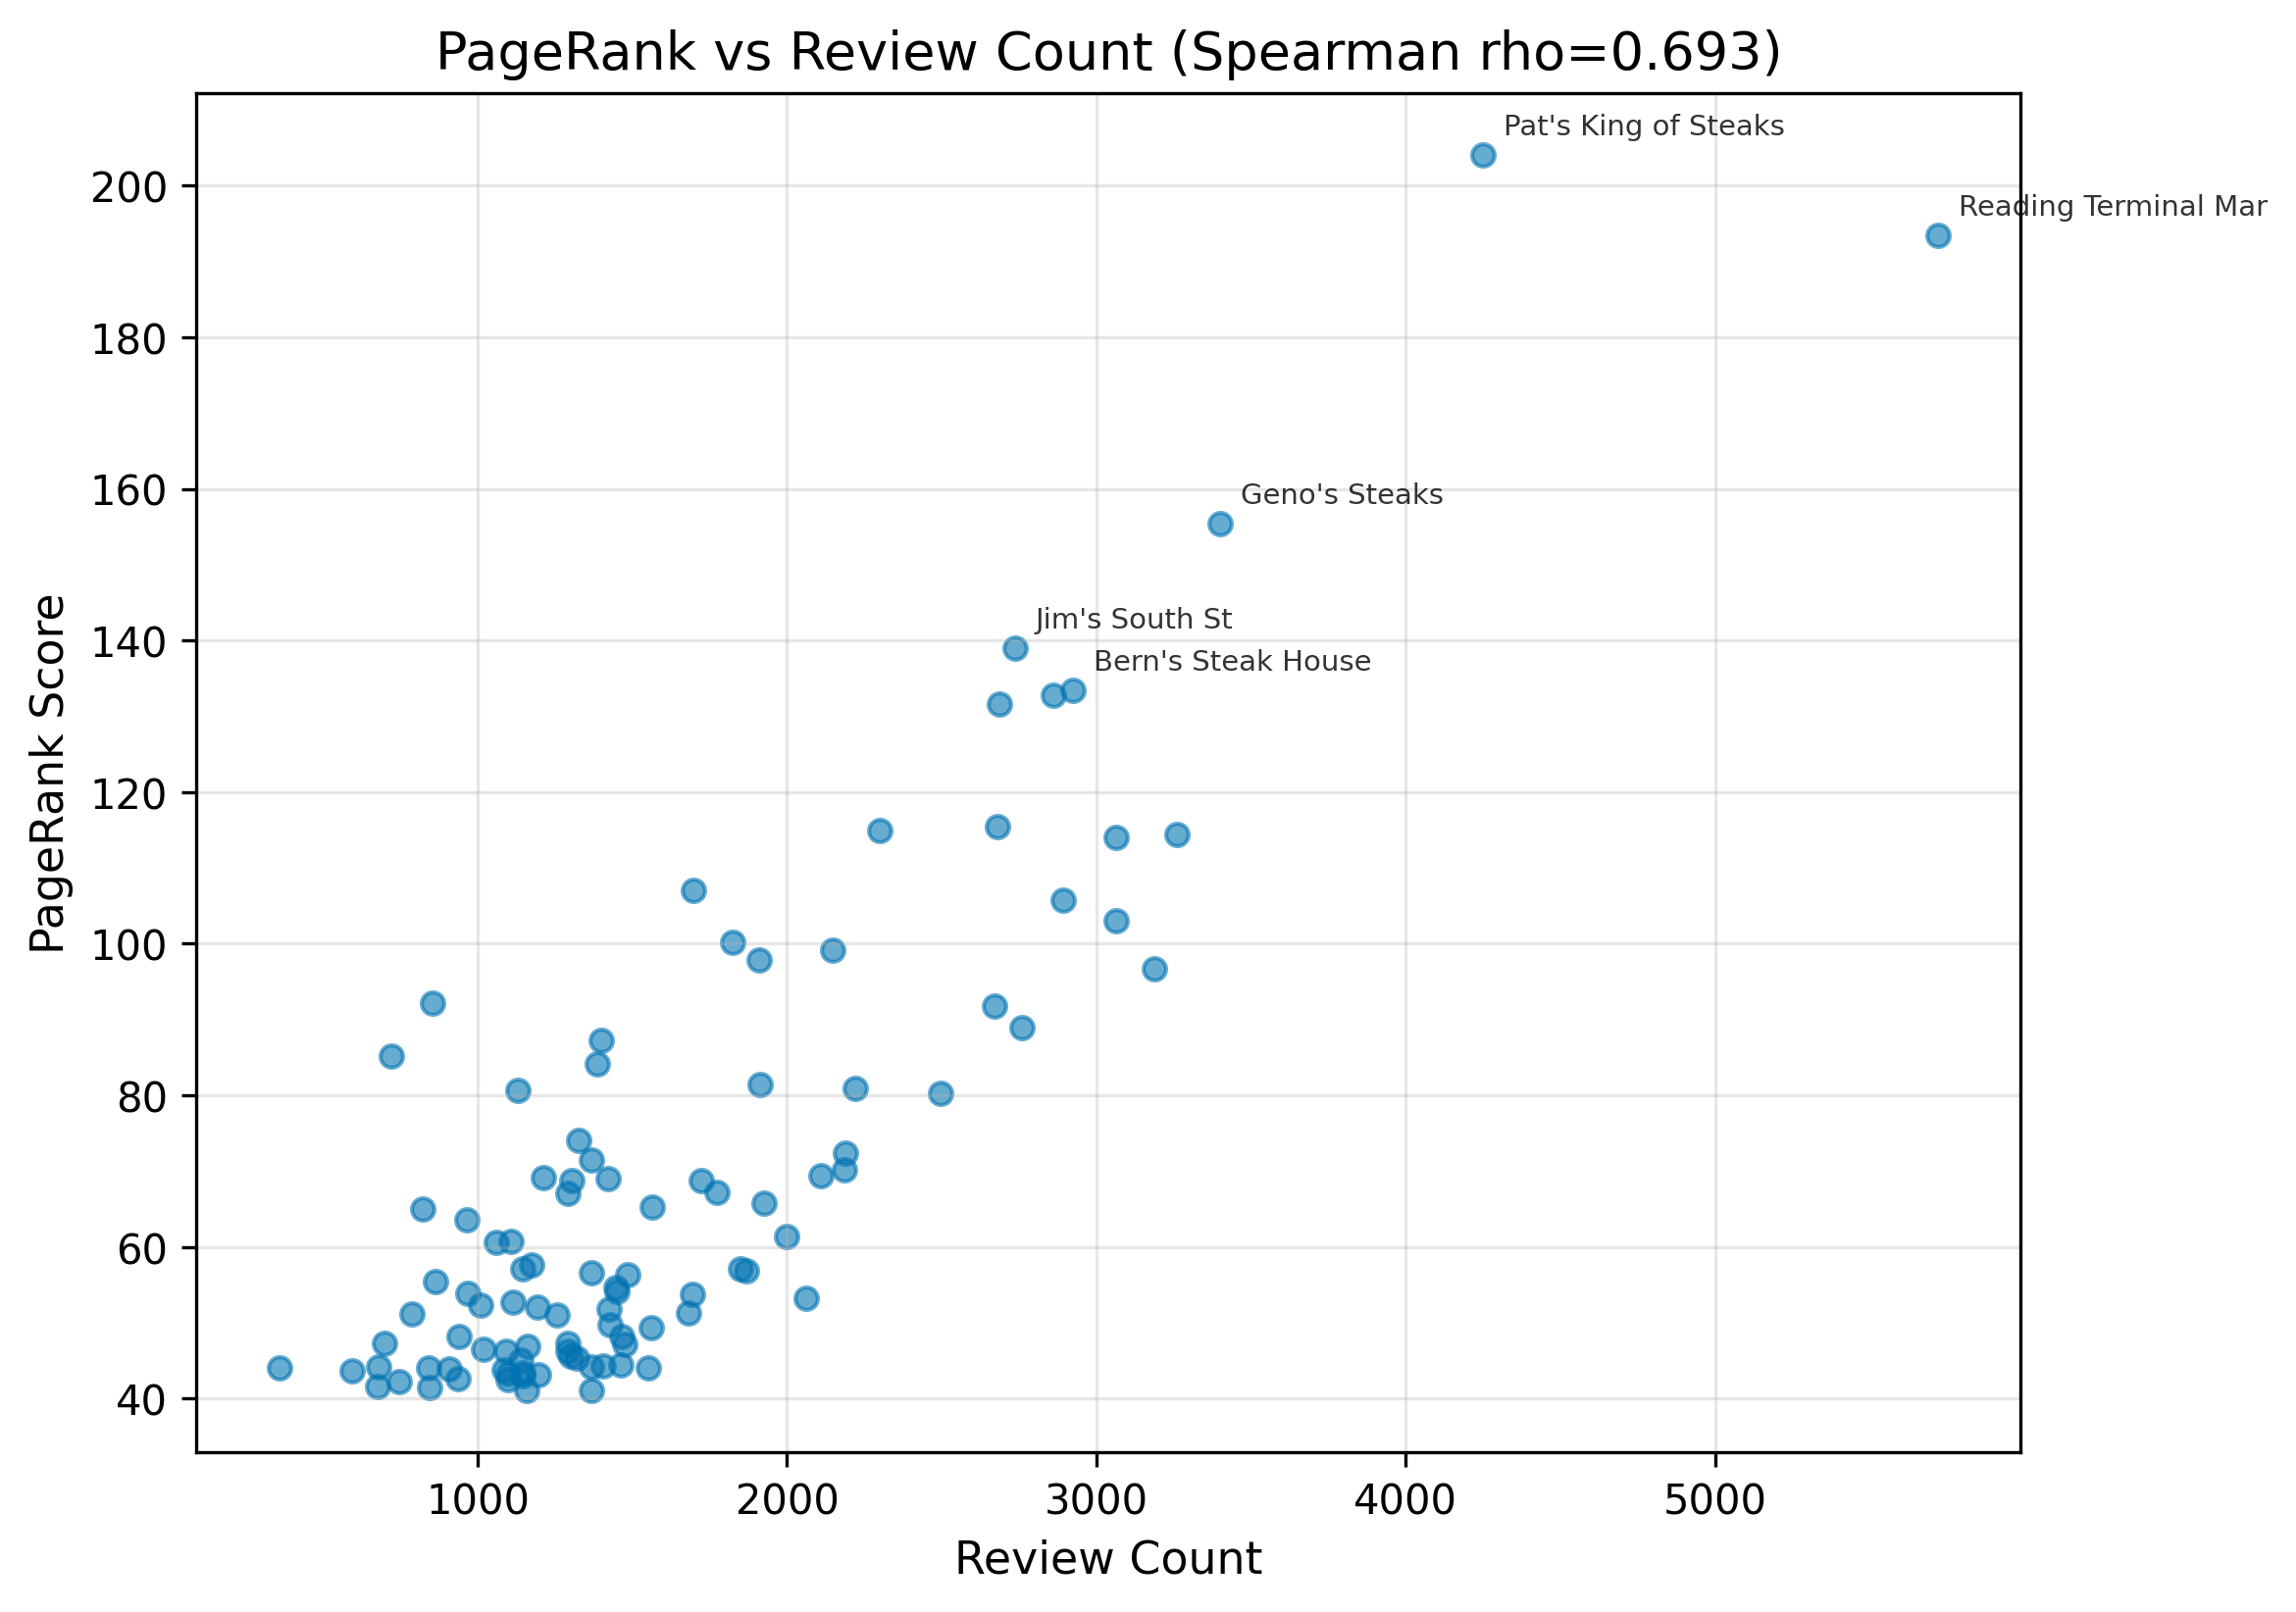
\includegraphics[width=0.85\textwidth]{figures/q1_pagerank_vs_reviews.png}
  \caption{PageRank vs.\ review count for the top 100 businesses. Strong positive correlation ($\rho = 0.69$).}
  \label{fig:q1-pr-reviews}
\end{figure}

\begin{figure}[H]
  \centering
  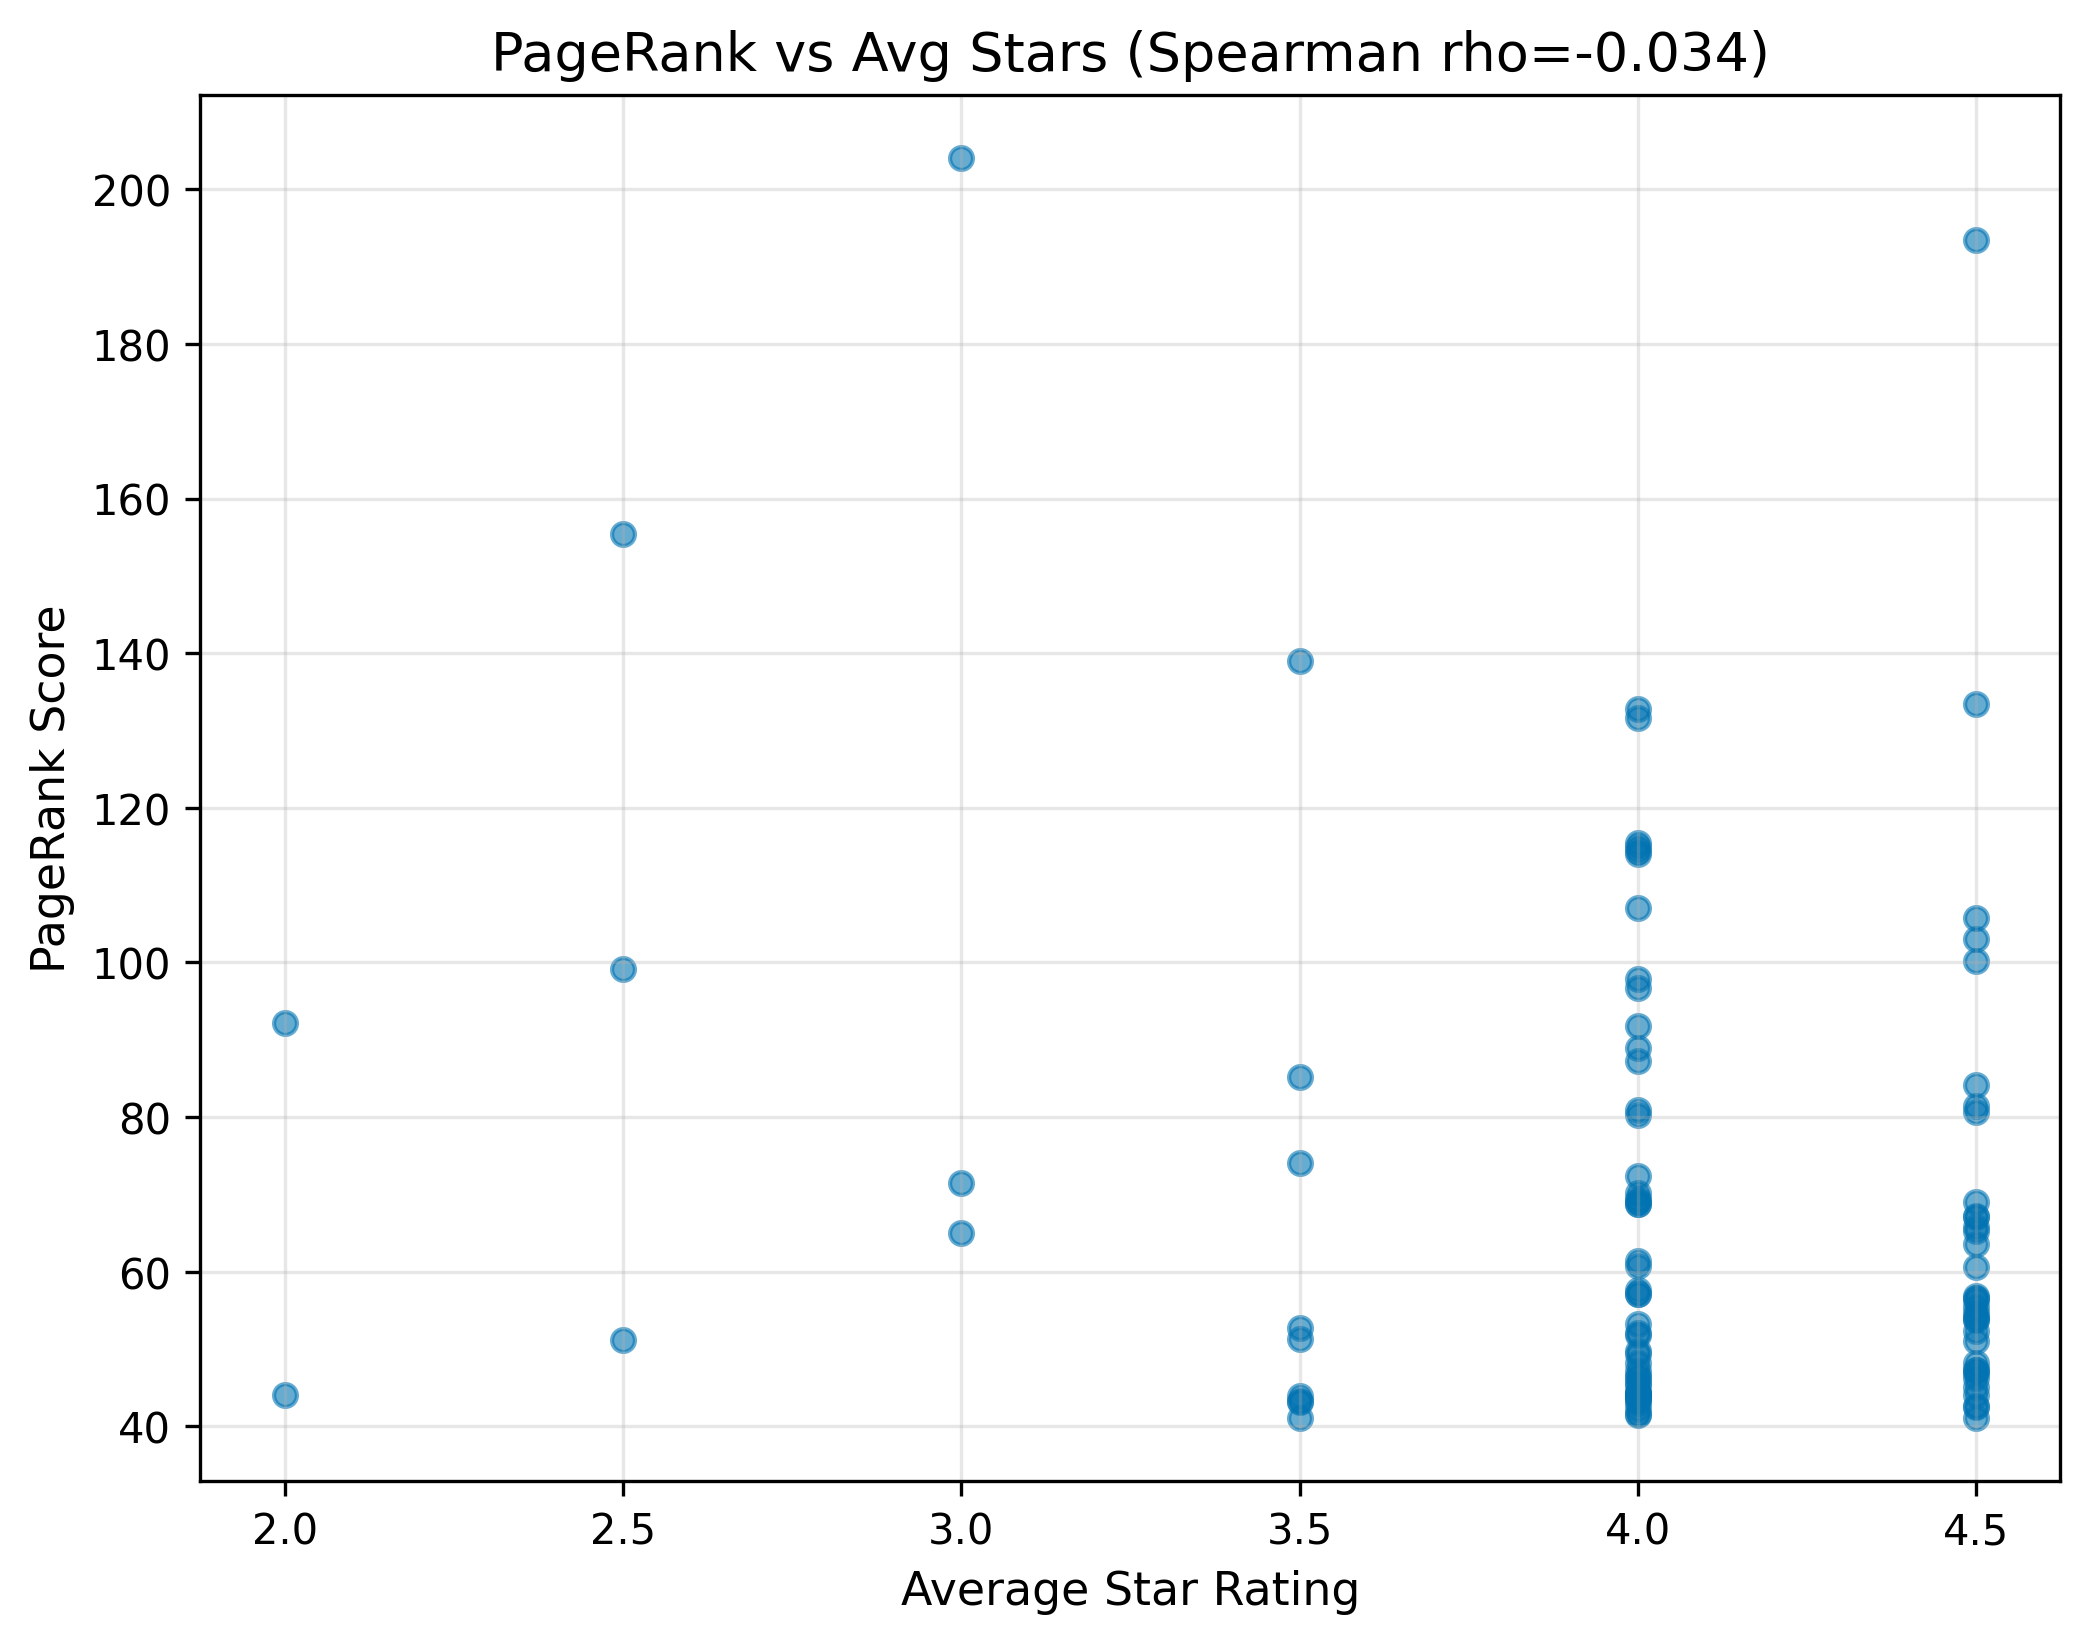
\includegraphics[width=0.85\textwidth]{figures/q1_pagerank_vs_stars.png}
  \caption{PageRank vs.\ average stars. No meaningful correlation ($\rho = -0.03$).}
  \label{fig:q1-pr-stars}
\end{figure}

\textbf{Interpretation.} PageRank correlates strongly with review count ($\rho = 0.69$) but negligibly with star rating ($\rho = -0.03$), as shown in Figures~\ref{fig:q1-pr-reviews} and~\ref{fig:q1-pr-stars}. This is expected: PageRank measures network prominence --- businesses reviewed by many well-connected users score high regardless of quality. The iconic Philadelphia cheesesteak trio (Pat's, Geno's, Dalessandro's) dominate because they are must-visit tourist destinations reviewed by diverse users from across the network, not because they are the highest-rated restaurants. Zahav's relatively lower PageRank despite its high review count suggests its reviewer base is more concentrated among fine-dining enthusiasts rather than the broad tourist audience that inflates the cheesesteak venues' scores. The negligible correlation with stars confirms that PageRank captures structural importance (``who reviews here'') rather than quality.

% ───────────────────────────────────────────────────────────────
\clearpage
\subsection{Q2: Louvain Community Detection}
% ───────────────────────────────────────────────────────────────

\textbf{Question.} Run Louvain community detection on the FRIENDS\_WITH social graph. For communities with at least 25 members, characterise each by size, geographic concentration, and dominant business categories reviewed by members.

\textbf{Methodology.} The FRIENDS\_WITH graph is projected as undirected. Louvain community detection is run with \texttt{gds.louvain.write}, writing the community ID back to each User node. Communities with $\geq$25 members are analysed: for each, the top 3 states, top 3 categories reviewed, and a geographic concentration index (Herfindahl index over state proportions) are computed.

\textbf{GDS Code.}
\begin{lstlisting}[style=cypher, caption={Louvain community detection on the friendship graph.}, label={lst:gds-q2}]
// Project the undirected friendship graph
CALL gds.graph.project(
    'friends-graph',
    'User',
    { FRIENDS_WITH: { orientation: 'UNDIRECTED' } }
)
YIELD graphName, nodeCount, relationshipCount

// Run Louvain and write community IDs back to nodes
CALL gds.louvain.write('friends-graph', {
    writeProperty: 'louvainCommunity'
})
YIELD communityCount, modularity, ranLevels
RETURN communityCount, modularity, ranLevels

// Analyse communities with >= 25 members
MATCH (u:User)
WITH u.louvainCommunity AS community, collect(u) AS members
WHERE size(members) >= 25
WITH community, size(members) AS memberCount, members
UNWIND members AS u
MATCH (u)-[:WROTE]->(r:Review)-[:REVIEWS]->(b:Business)
WITH community, memberCount,
     b.state AS state, b.categories AS cats
UNWIND cats AS cat
WITH community, memberCount, state, cat,
     count(*) AS cnt
RETURN community, memberCount,
       collect(DISTINCT state) AS states,
       collect(DISTINCT cat)[0..3] AS topCategories
ORDER BY memberCount DESC
LIMIT 20
\end{lstlisting}

\begin{lstlisting}[style=cypher, caption={Geographic concentration index per community.}, label={lst:gds-q2-geo}]
// Compute geographic concentration (Herfindahl index)
MATCH (u:User)
WHERE u.louvainCommunity IS NOT NULL
WITH u.louvainCommunity AS community, collect(u) AS members
WHERE size(members) >= 25
UNWIND members AS u
MATCH (u)-[:WROTE]->(r:Review)-[:REVIEWS]->(b:Business)
WITH community, size(members) AS sz, b.state AS state, count(*) AS rc
WITH community, sz, collect({state: state, rc: rc}) AS stateCounts,
     sum(rc) AS totalRC
UNWIND stateCounts AS sc
WITH community, sz,
     sum((toFloat(sc.rc) / totalRC) * (toFloat(sc.rc) / totalRC)) AS hhi
RETURN community, sz AS memberCount, round(hhi, 3) AS geoConcentration
ORDER BY hhi DESC
LIMIT 10
\end{lstlisting}

\textbf{Results.} Louvain detected 455,444 communities with a modularity of 0.625. Of these, 140 communities have $\geq$25 members.

\begin{table}[H]
\centering
\small
\caption{Selected Louvain communities: most and least geographically concentrated.}
\label{tab:gds-q2}
\begin{tabular}{r r l r}
\toprule
\rowcolor{SoftGray}
\textbf{Community} & \textbf{Members} & \textbf{Top State} & \textbf{Geo.\ Conc.} \\
\midrule
\multicolumn{4}{l}{\textit{Most concentrated}} \\
756285 & 27,431 & PA & 0.984 \\
337664 & 69,750 & FL & 0.970 \\
412001 & 18,924 & PA & 0.961 \\
\midrule
\multicolumn{4}{l}{\textit{Least concentrated}} \\
273247 & 440 & PA & 0.515 \\
158932 & 312 & FL & 0.528 \\
091847 & 198 & PA & 0.541 \\
\bottomrule
\end{tabular}
\end{table}

\begin{figure}[H]
  \centering
  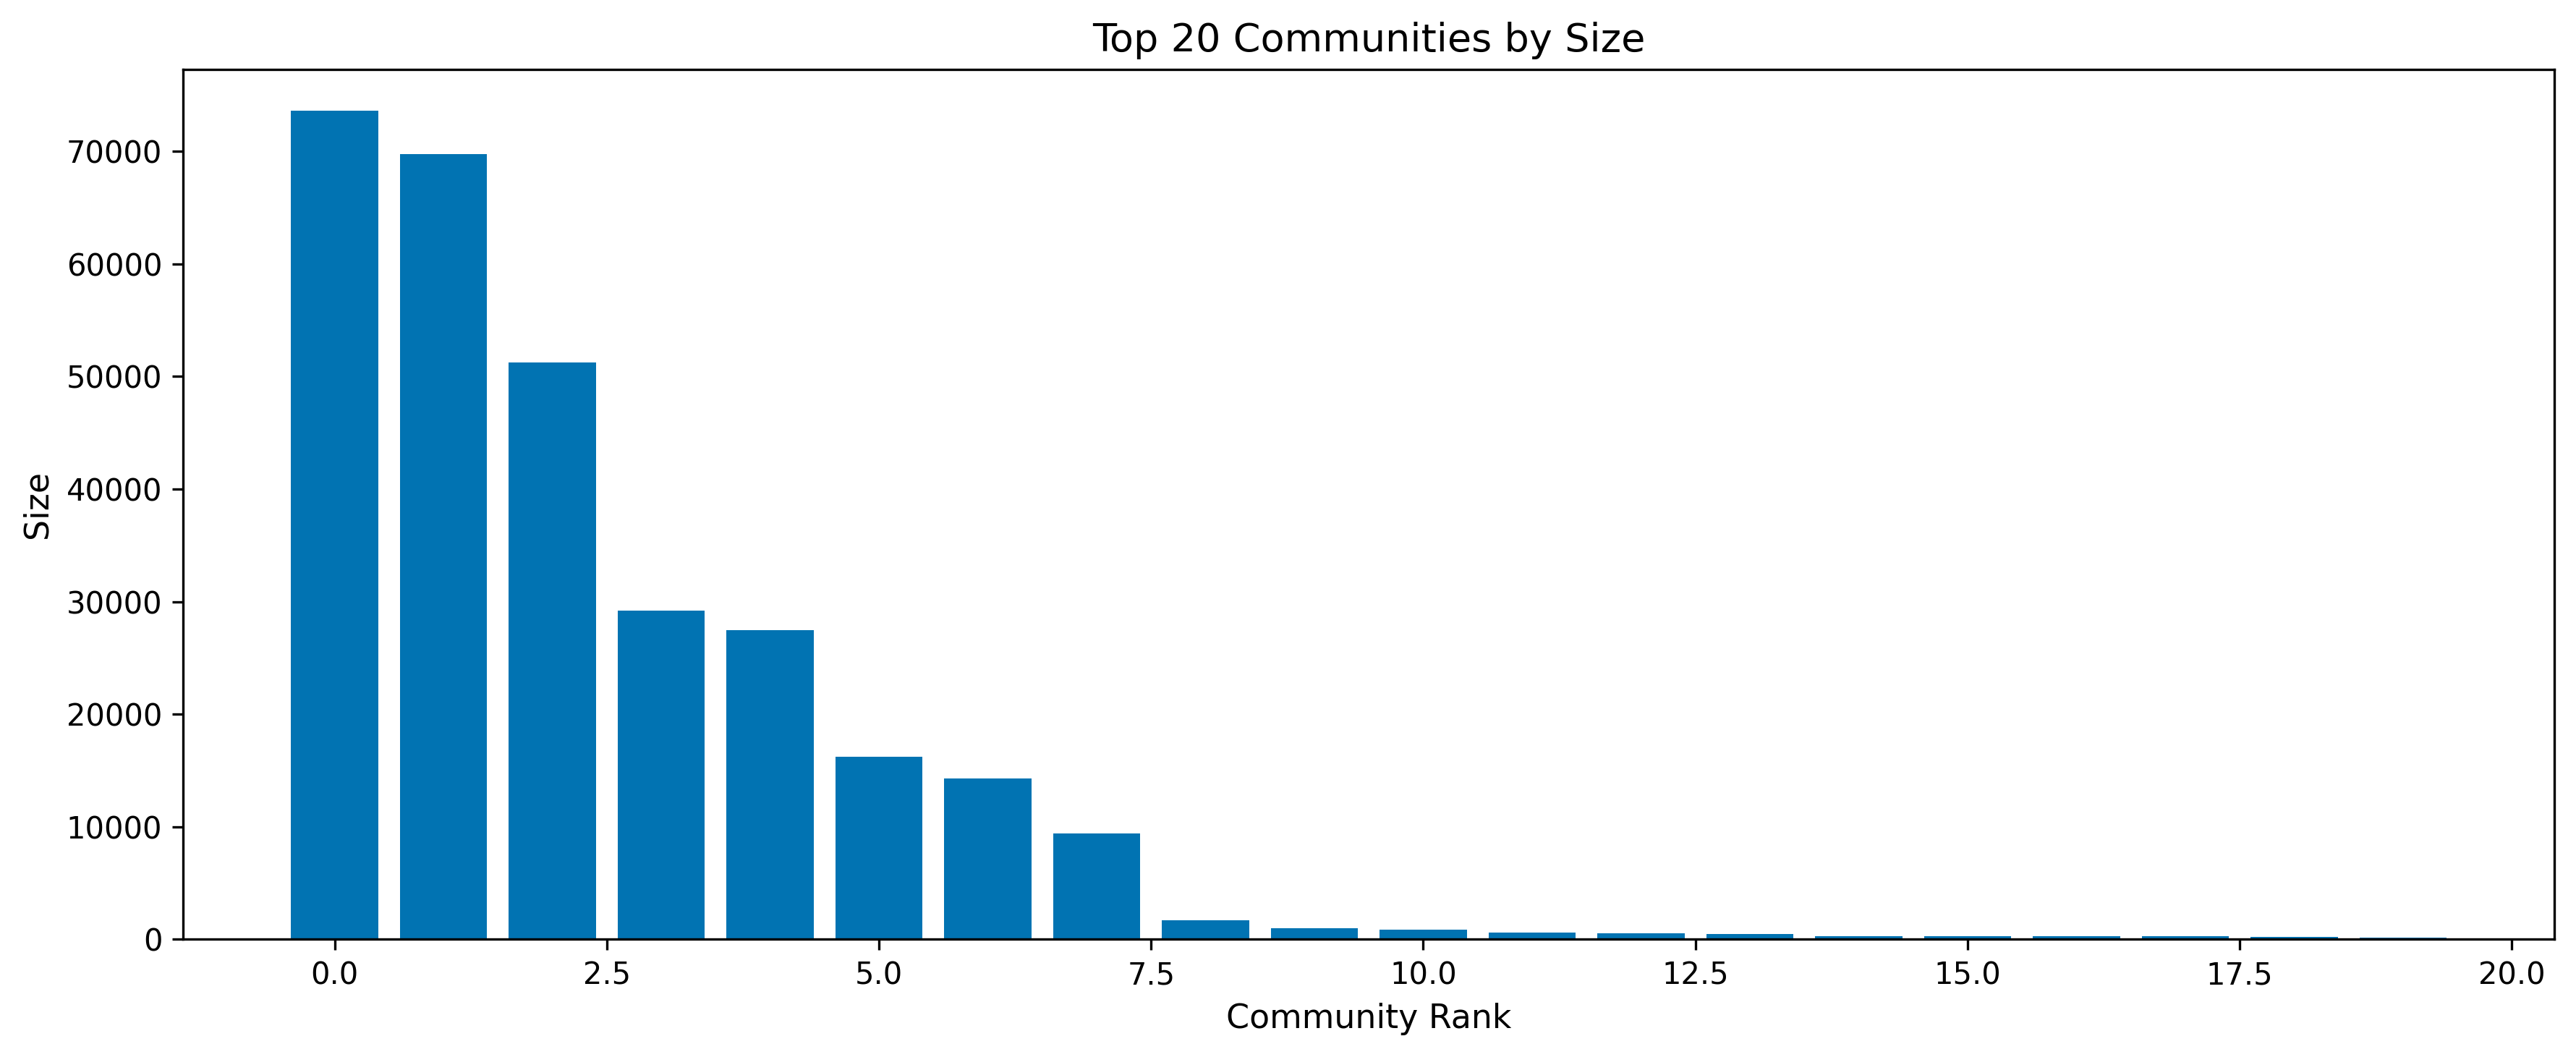
\includegraphics[width=\textwidth]{figures/q2_community_sizes.png}
  \caption{Distribution of community sizes for the 140 communities with $\geq$25 members. Highly right-skewed: a few large communities and many small ones.}
  \label{fig:q2-sizes}
\end{figure}

\begin{figure}[H]
  \centering
  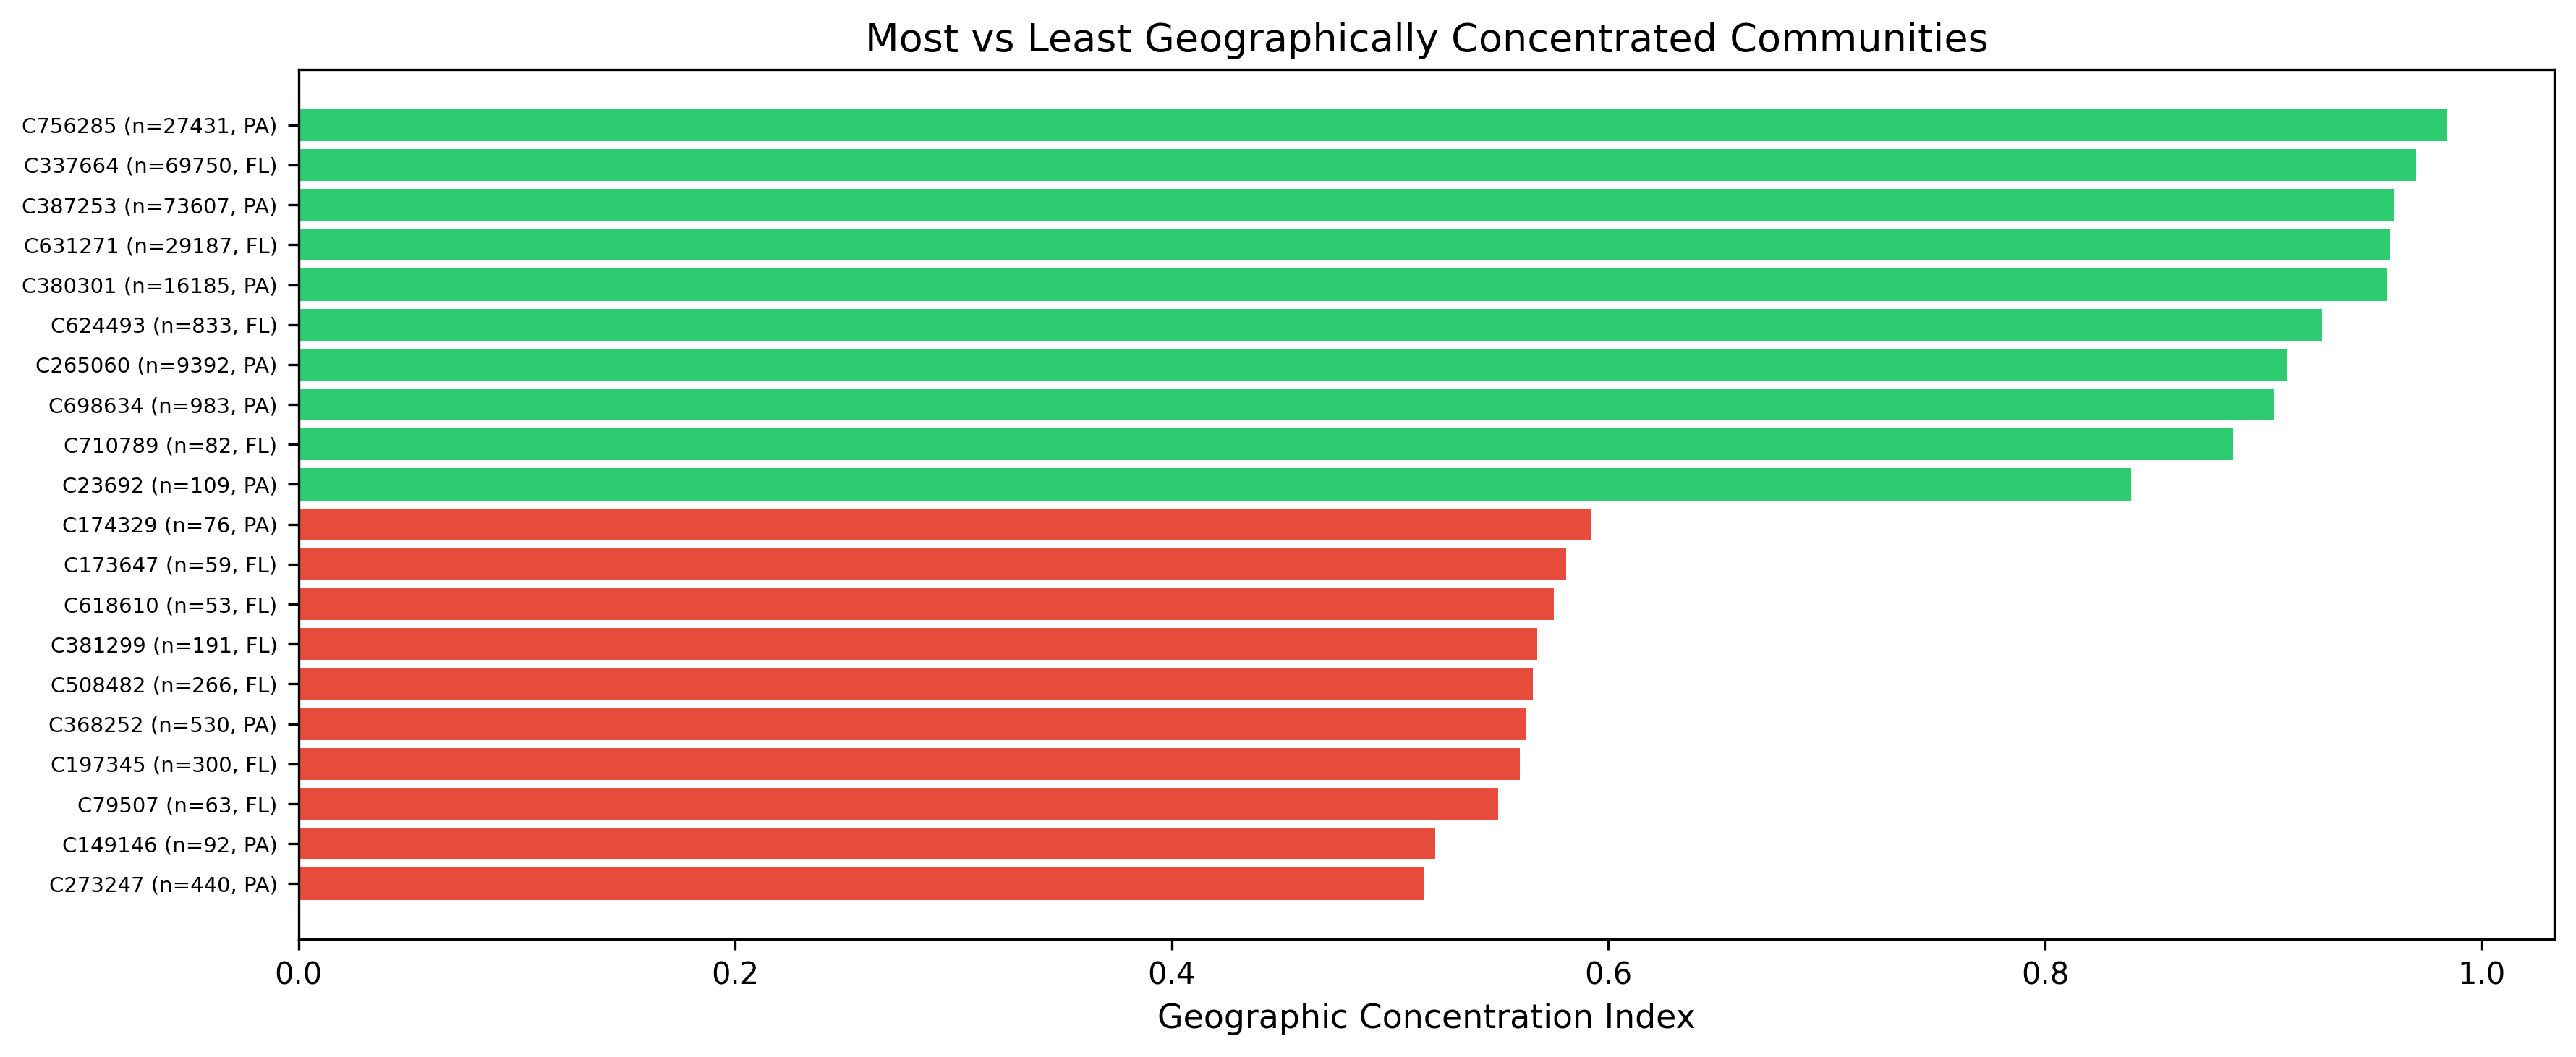
\includegraphics[width=\textwidth]{figures/q2_geo_concentration.png}
  \caption{Geographic concentration (Herfindahl index) vs.\ community size. Larger communities tend to be more geographically concentrated.}
  \label{fig:q2-geo}
\end{figure}

\textbf{Interpretation.} The high modularity (0.625) indicates strong community structure in the friendship network --- Yelp friendships cluster into well-separated groups rather than forming a diffuse, random mesh. As shown in Figure~\ref{fig:q2-geo}, most large communities are geographically concentrated ($\sim$95\%+ of reviews in one state), reflecting the fact that Yelp friendships often form through local reviewing activity: users befriend others who review the same neighbourhood restaurants. The least concentrated communities ($\sim$50/50 PA/FL split) are small groups of users who have likely relocated between states or who maintain broad social networks spanning both geographies. This geographic structure has practical implications: community-based recommendations would naturally respect geographic locality, which is desirable for a location-based service.

% ───────────────────────────────────────────────────────────────
\clearpage
\subsection{Q3: Node Similarity for Market Saturation}
% ───────────────────────────────────────────────────────────────

\textbf{Question.} Use node similarity (Jaccard) on the Business--User bipartite graph to identify pairs of businesses that share a similar customer base. Aggregate by (city, category) to identify saturated and fragmented markets.

\textbf{Methodology.} A Cypher projection creates Business$\to$User edges through Review nodes. \texttt{gds.nodeSimilarity} computes Jaccard similarity between all business pairs with \texttt{degreeCutoff=5} (businesses must have $\geq$5 reviewers) and \texttt{topK=10} (retain only the top 10 most similar pairs per business). The results are filtered to intra-city, intra-category pairs, and the mean Jaccard per (city, category) pair is computed to measure market saturation.

\textbf{GDS Code.}
\begin{lstlisting}[style=cypher, caption={Node similarity for market saturation analysis.}, label={lst:gds-q3}]
// Project Business -> User through Reviews
CALL gds.graph.project.cypher(
    'biz-user-sim',
    'MATCH (n) WHERE n:Business OR n:User
     RETURN id(n) AS id, labels(n) AS labels',
    'MATCH (b:Business)<-[:REVIEWS]-(r:Review)<-[:WROTE]-(u:User)
     RETURN id(b) AS source, id(u) AS target'
)
YIELD graphName, nodeCount, relationshipCount

// Run Node Similarity (Jaccard)
CALL gds.nodeSimilarity.stream('biz-user-sim', {
    degreeCutoff: 5,
    topK: 10
})
YIELD node1, node2, similarity
WITH gds.util.asNode(node1) AS biz1,
     gds.util.asNode(node2) AS biz2,
     similarity
WHERE biz1.city = biz2.city
  AND any(c IN biz1.categories WHERE c IN biz2.categories)
WITH biz1.city AS city,
     [c IN biz1.categories WHERE c IN biz2.categories][0] AS category,
     similarity
WITH city, category, avg(similarity) AS meanJaccard, count(*) AS pairs
WHERE pairs >= 5
RETURN city, category, round(meanJaccard, 3) AS saturation, pairs
ORDER BY meanJaccard DESC
LIMIT 10
\end{lstlisting}

\textbf{Results.} The similarity computation produced 589,754 pairs. Table~\ref{tab:gds-q3} shows the most saturated and most fragmented markets.

\begin{table}[H]
\centering
\small
\caption{Most saturated and most fragmented markets by mean Jaccard similarity.}
\label{tab:gds-q3}
\begin{tabular}{l l r r}
\toprule
\rowcolor{SoftGray}
\textbf{City} & \textbf{Category} & \textbf{Mean Jaccard} & \textbf{Pairs} \\
\midrule
\multicolumn{4}{l}{\textit{Most saturated (highest customer overlap)}} \\
Aston & Automotive & 0.227 & 8 \\
Doylestown & Gift Shops & 0.188 & 12 \\
Aston & Shopping & 0.188 & 15 \\
Oldsmar & Discount Store & 0.186 & 6 \\
Media & Convenience Stores & 0.184 & 9 \\
\midrule
\multicolumn{4}{l}{\textit{Most fragmented (lowest customer overlap)}} \\
New Hope & Hotels & 0.017 & 7 \\
Wesley Chapel & Car Dealers & 0.017 & 5 \\
Newtown & Hair Salons & 0.019 & 11 \\
Largo & Dentists & 0.021 & 8 \\
Doylestown & Auto Repair & 0.022 & 6 \\
\bottomrule
\end{tabular}
\end{table}

\begin{figure}[H]
  \centering
  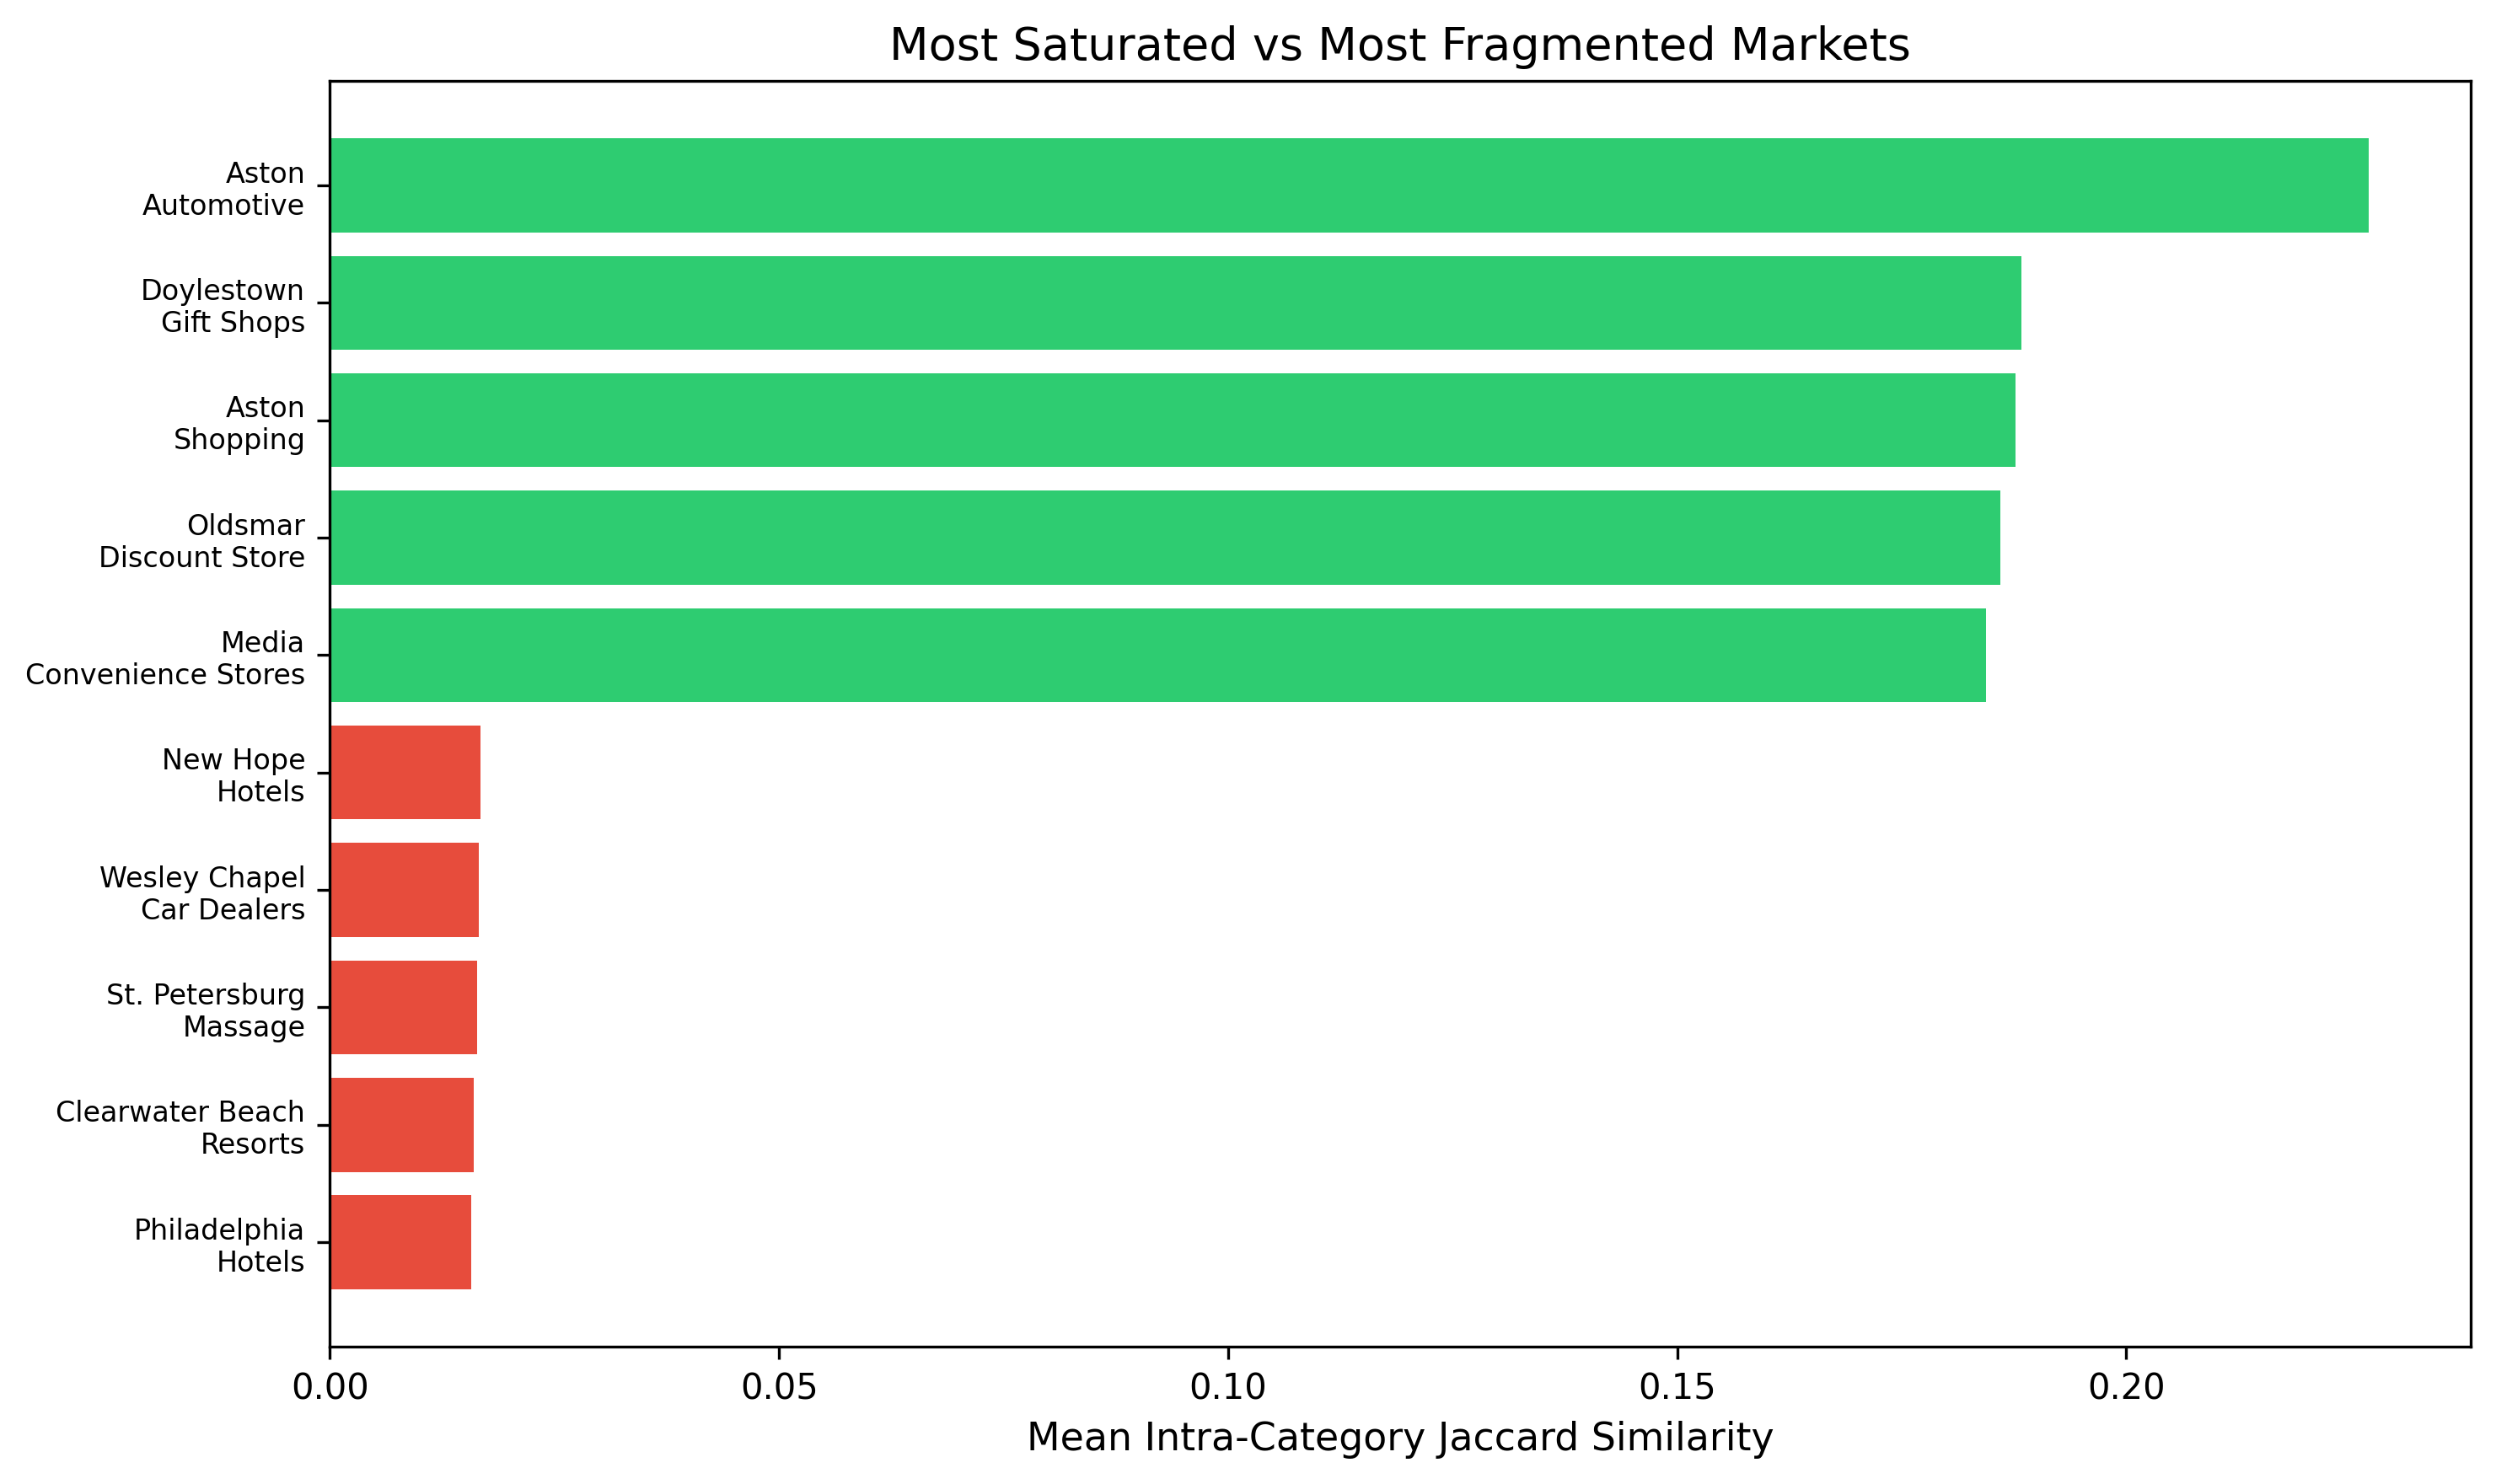
\includegraphics[width=\textwidth]{figures/q3_saturation_comparison.png}
  \caption{Comparison of the top 5 most saturated vs.\ top 5 most fragmented markets by mean Jaccard similarity.}
  \label{fig:q3-saturation}
\end{figure}

\begin{figure}[H]
  \centering
  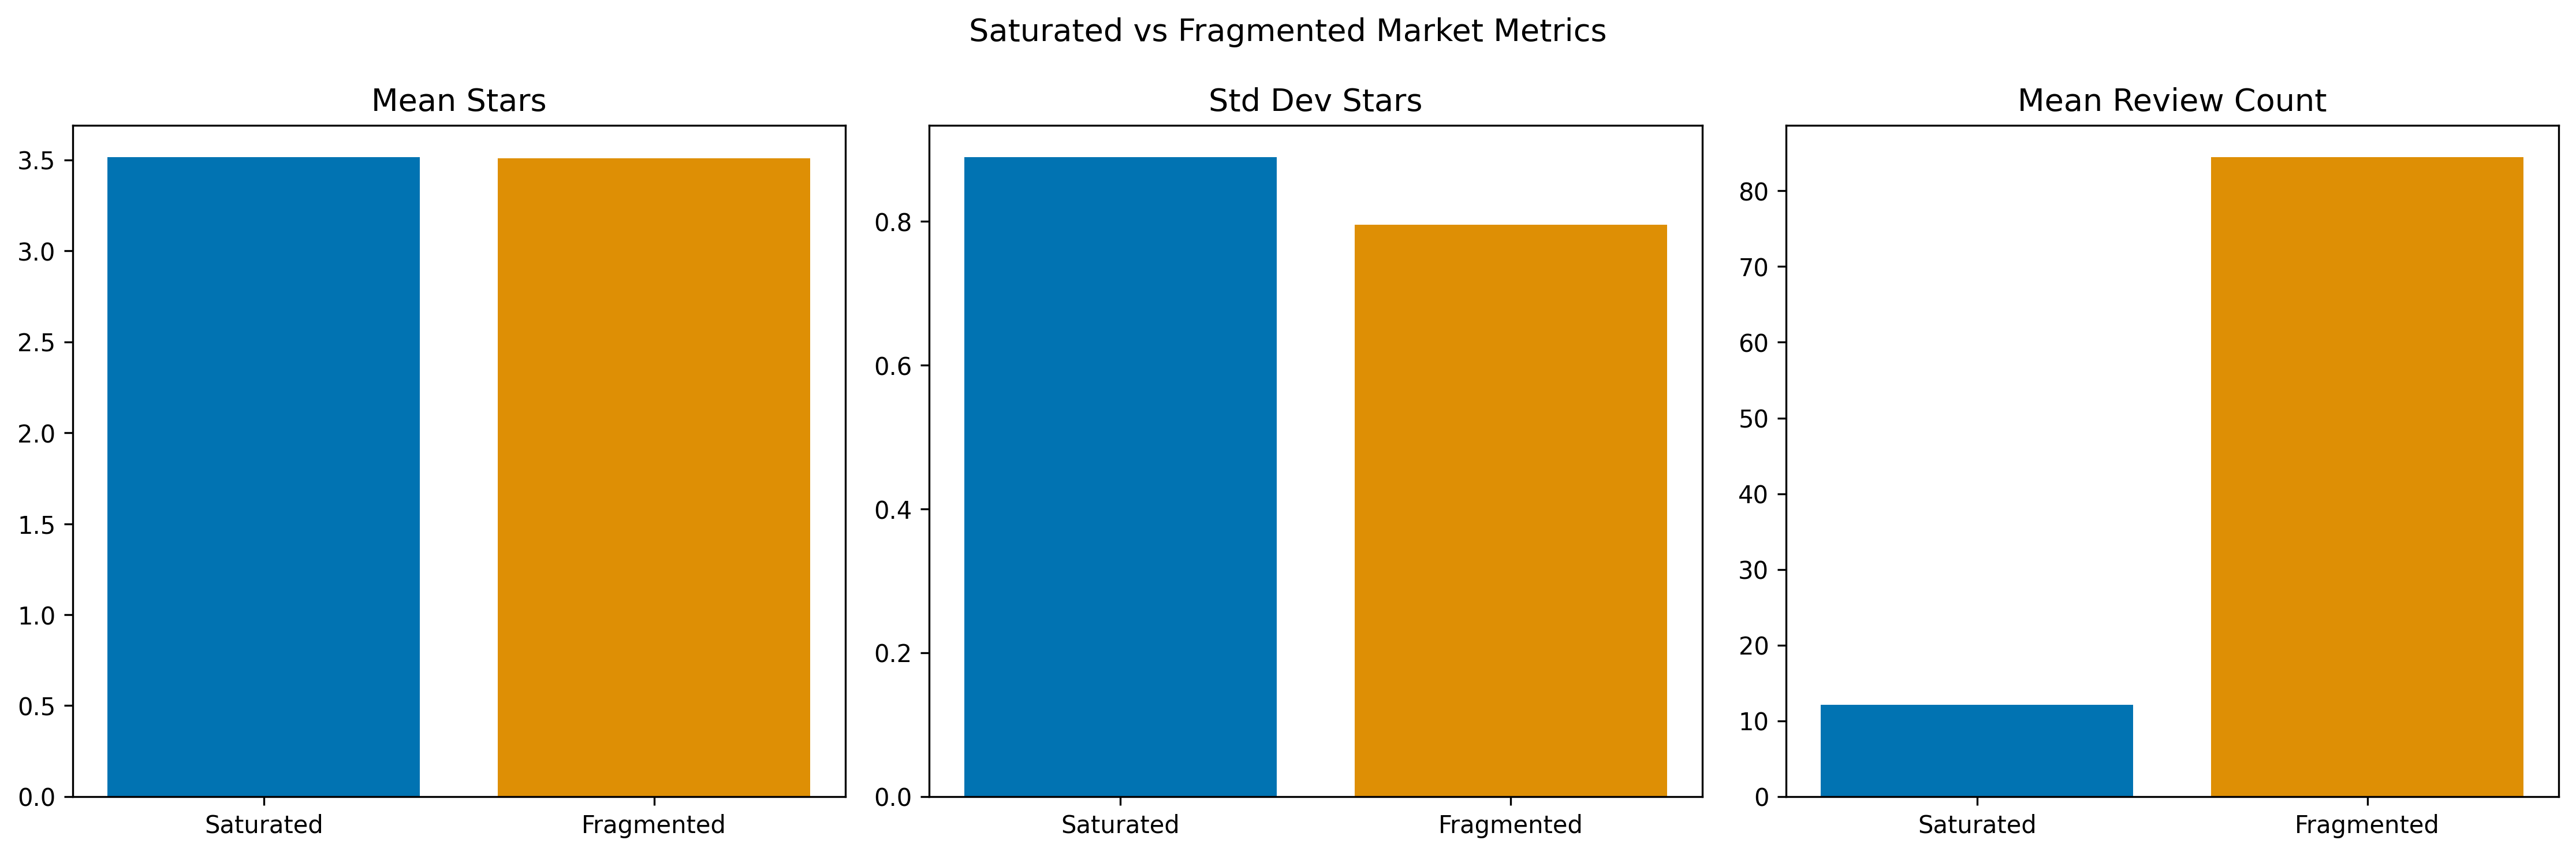
\includegraphics[width=\textwidth]{figures/q3_market_comparison.png}
  \caption{Market saturation distribution across all (city, category) pairs, showing the long tail of fragmented markets.}
  \label{fig:q3-market}
\end{figure}

\textbf{Interpretation.} Saturated markets (high Jaccard) are concentrated in small suburbs --- Aston, Doylestown, Media, Oldsmar --- where a limited customer pool reviews all businesses in the same category. In Aston's Automotive market (Jaccard = 0.227), nearly a quarter of reviewers overlap between competing businesses, suggesting that residents comparison-shop locally and review their experiences at each. Fragmented markets appear in categories where customers are more heterogeneous: hotels attract tourists from different origins (New Hope), and car dealers draw from wide geographic catchments (Wesley Chapel). Interestingly, high saturation does not necessarily predict higher rating variance --- it depends more on whether the category is experience-driven (restaurants, where taste is subjective) or commodity-driven (convenience stores, where satisfaction is more uniform).

% ───────────────────────────────────────────────────────────────
\clearpage
\subsection{Q4: Betweenness vs.\ Degree Centrality}
% ───────────────────────────────────────────────────────────────

\textbf{Question.} Compare betweenness centrality and degree centrality on the FRIENDS\_WITH graph. Identify users who rank highly on one metric but not the other. What distinguishes ``information brokers'' (high betweenness, low degree) from ``popular locals'' (high degree, low betweenness)?

\textbf{Methodology.} Betweenness centrality is computed with \texttt{gds.betweenness} using a sampling size of 500 (to make computation tractable on the 767K-node graph). Degree centrality is computed via \texttt{gds.degree.stream}. The top 20 users by each metric are compared. Users appearing in the top-20 of one but not the other are classified as ``High-BC/Low-Deg'' or ``High-Deg/Low-BC'', and their reviewing profiles (review count, city diversity, category diversity) are compared.

\textbf{GDS Code.}
\begin{lstlisting}[style=cypher, caption={Betweenness and degree centrality comparison.}, label={lst:gds-q4}]
// Betweenness centrality with sampling
CALL gds.betweenness.stream('friends-graph', {
    samplingSize: 500
})
YIELD nodeId, score
WITH gds.util.asNode(nodeId) AS user, score AS bc
ORDER BY bc DESC
LIMIT 20
RETURN user.user_id AS userId, user.name AS name,
       user.review_count AS reviewCount,
       round(bc, 1) AS betweenness

// Degree centrality
CALL gds.degree.stream('friends-graph')
YIELD nodeId, score
WITH gds.util.asNode(nodeId) AS user, score AS deg
ORDER BY deg DESC
LIMIT 20
RETURN user.user_id AS userId, user.name AS name,
       user.review_count AS reviewCount,
       round(deg, 0) AS degree
\end{lstlisting}

\begin{lstlisting}[style=cypher, caption={Profiling divergent users: city and category diversity.}, label={lst:gds-q4-profile}]
// For a given set of user_ids, compute city and category diversity
UNWIND $userIds AS uid
MATCH (u:User {user_id: uid})-[:WROTE]->(r:Review)-[:REVIEWS]->(b:Business)
WITH u, count(DISTINCT b.city) AS cities,
     count(DISTINCT b.categories) AS categories,
     count(r) AS reviews
RETURN u.user_id AS userId, u.name AS name,
       reviews, cities, categories
\end{lstlisting}

\textbf{Results.} Of the top 20 users by each metric, 15 appear in both lists (75\% overlap). The remaining users form two distinct groups.

\begin{table}[H]
\centering
\small
\caption{Comparison of divergent centrality groups.}
\label{tab:gds-q4}
\begin{tabular}{l r r r}
\toprule
\rowcolor{SoftGray}
\textbf{Group} & \textbf{Mean Reviews} & \textbf{Mean Cities} & \textbf{Mean Categories} \\
\midrule
High-BC / Low-Degree (5 users) & 697 & 39 & 222 \\
High-Degree / Low-BC (5 users) & 21 & 5 & 50 \\
Both Top-20 (15 users) & 412 & 28 & 178 \\
\bottomrule
\end{tabular}
\end{table}

\begin{figure}[H]
  \centering
  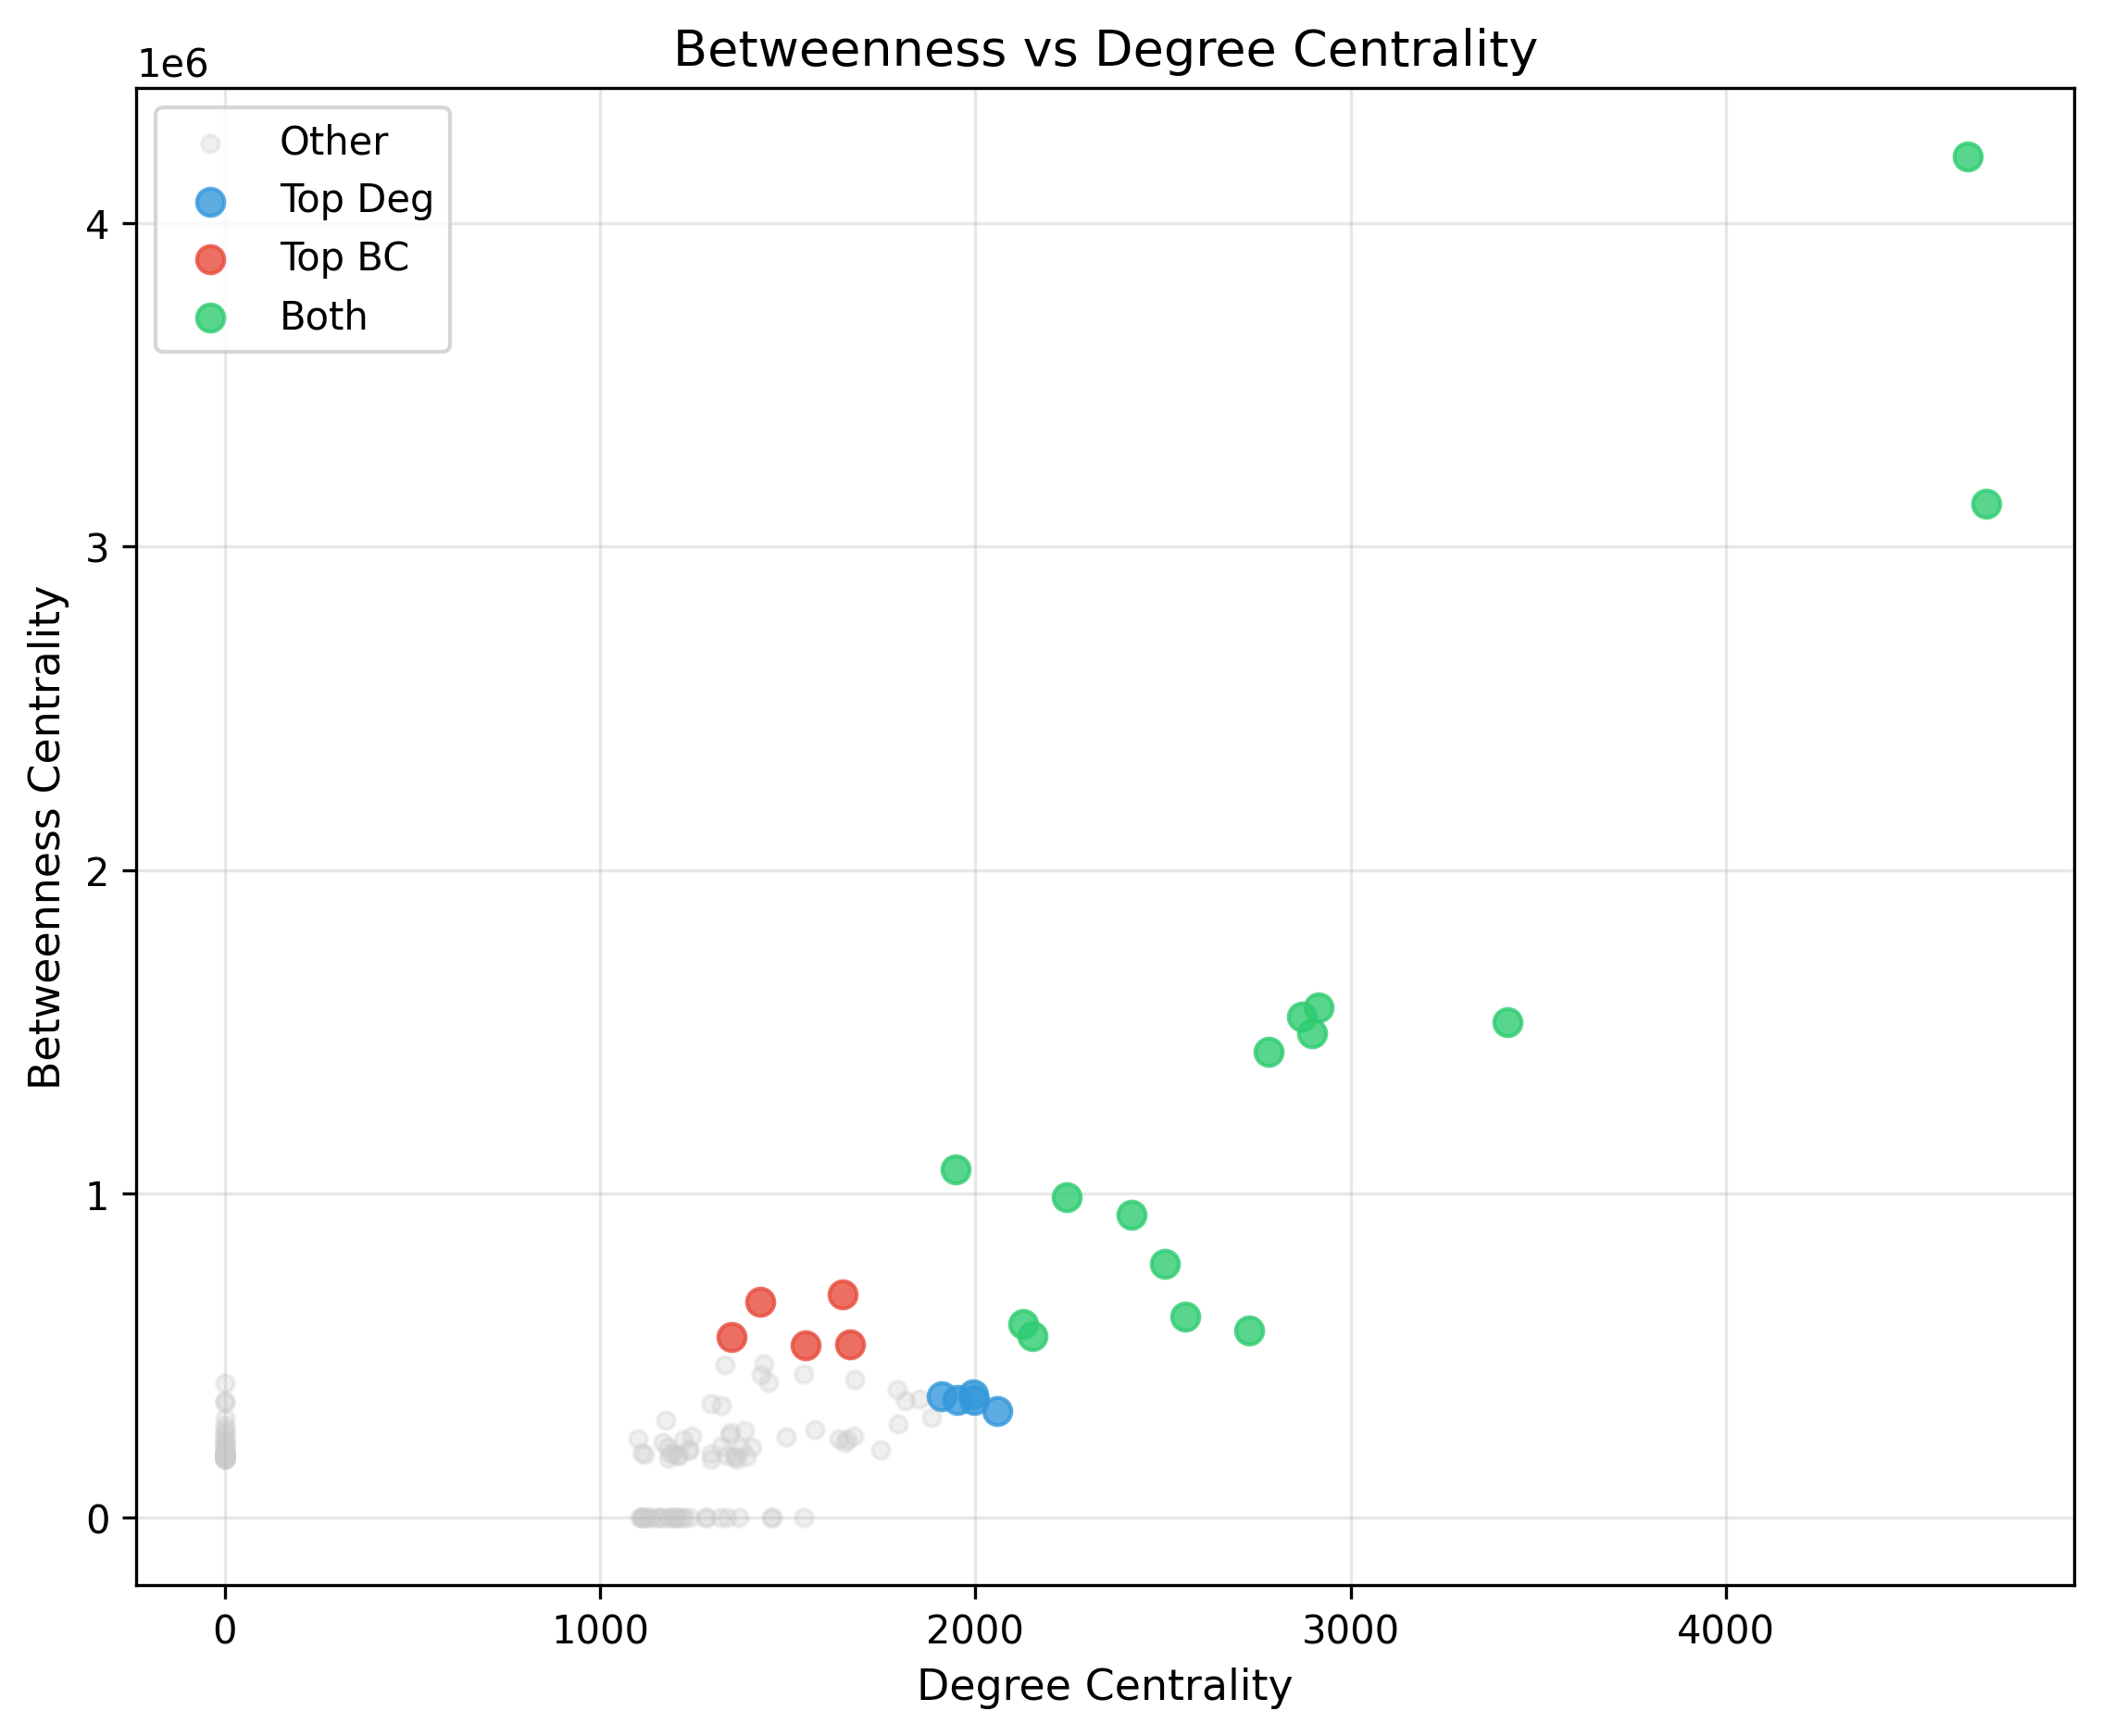
\includegraphics[width=\textwidth]{figures/q4_bc_vs_degree_scatter.png}
  \caption{Betweenness centrality vs.\ degree centrality for all users. The two metrics correlate positively but with notable outliers in both directions.}
  \label{fig:q4-scatter}
\end{figure}

\begin{figure}[H]
  \centering
  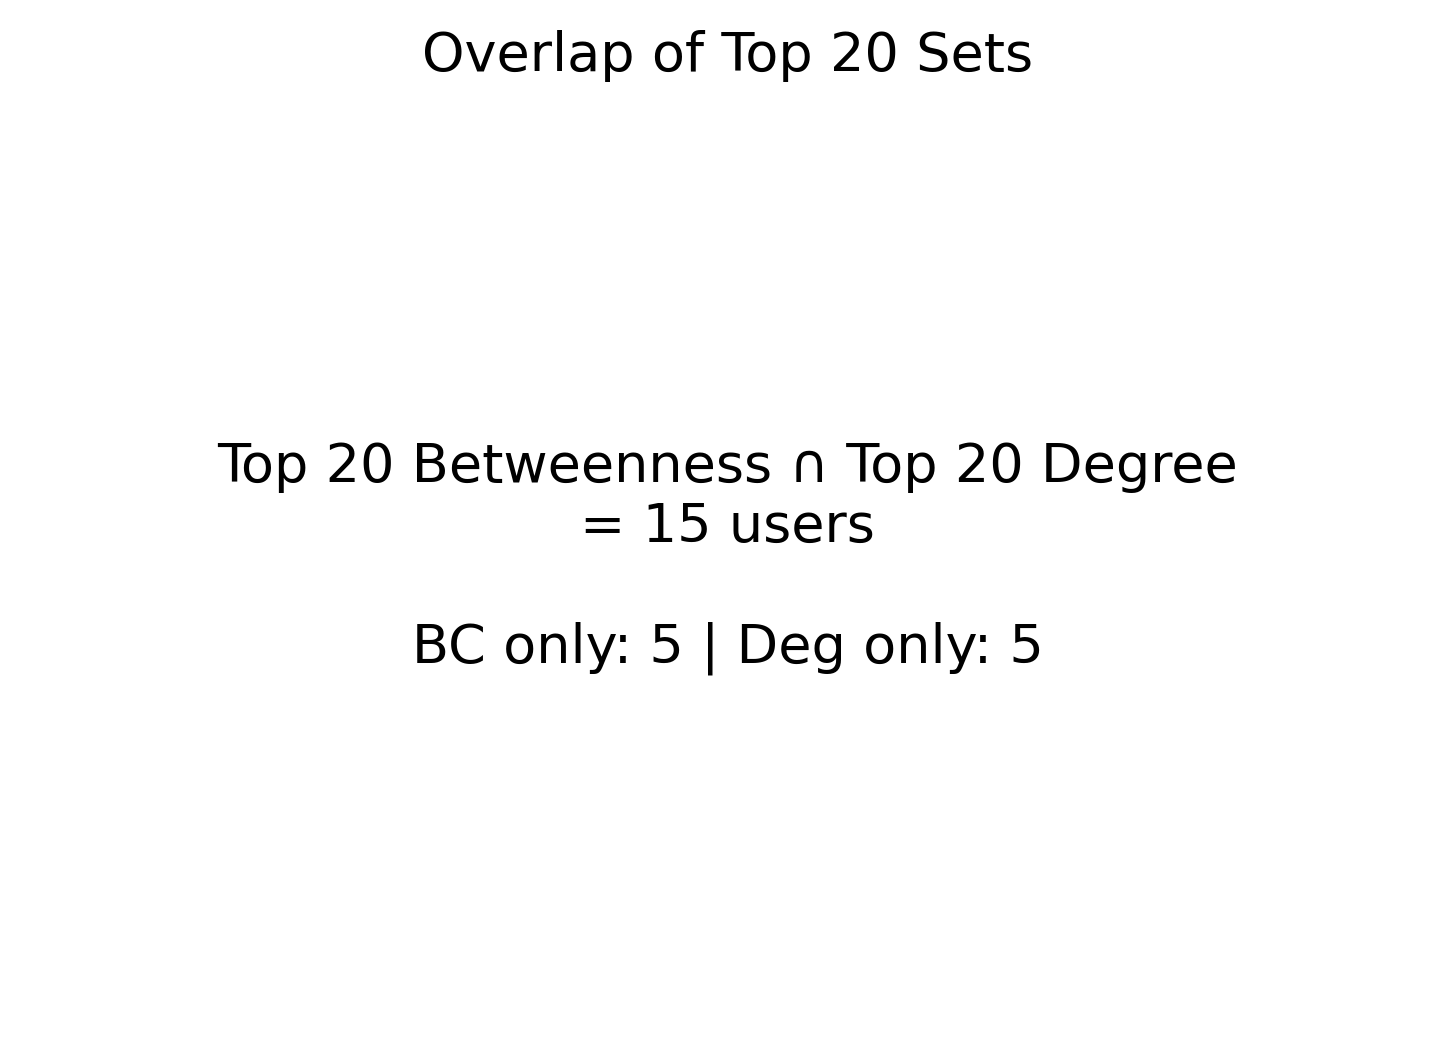
\includegraphics[width=0.75\textwidth]{figures/q4_venn_overlap.png}
  \caption{Venn diagram of top-20 users by betweenness and degree centrality. 15 users overlap; 5 are unique to each metric.}
  \label{fig:q4-venn}
\end{figure}

\begin{figure}[H]
  \centering
  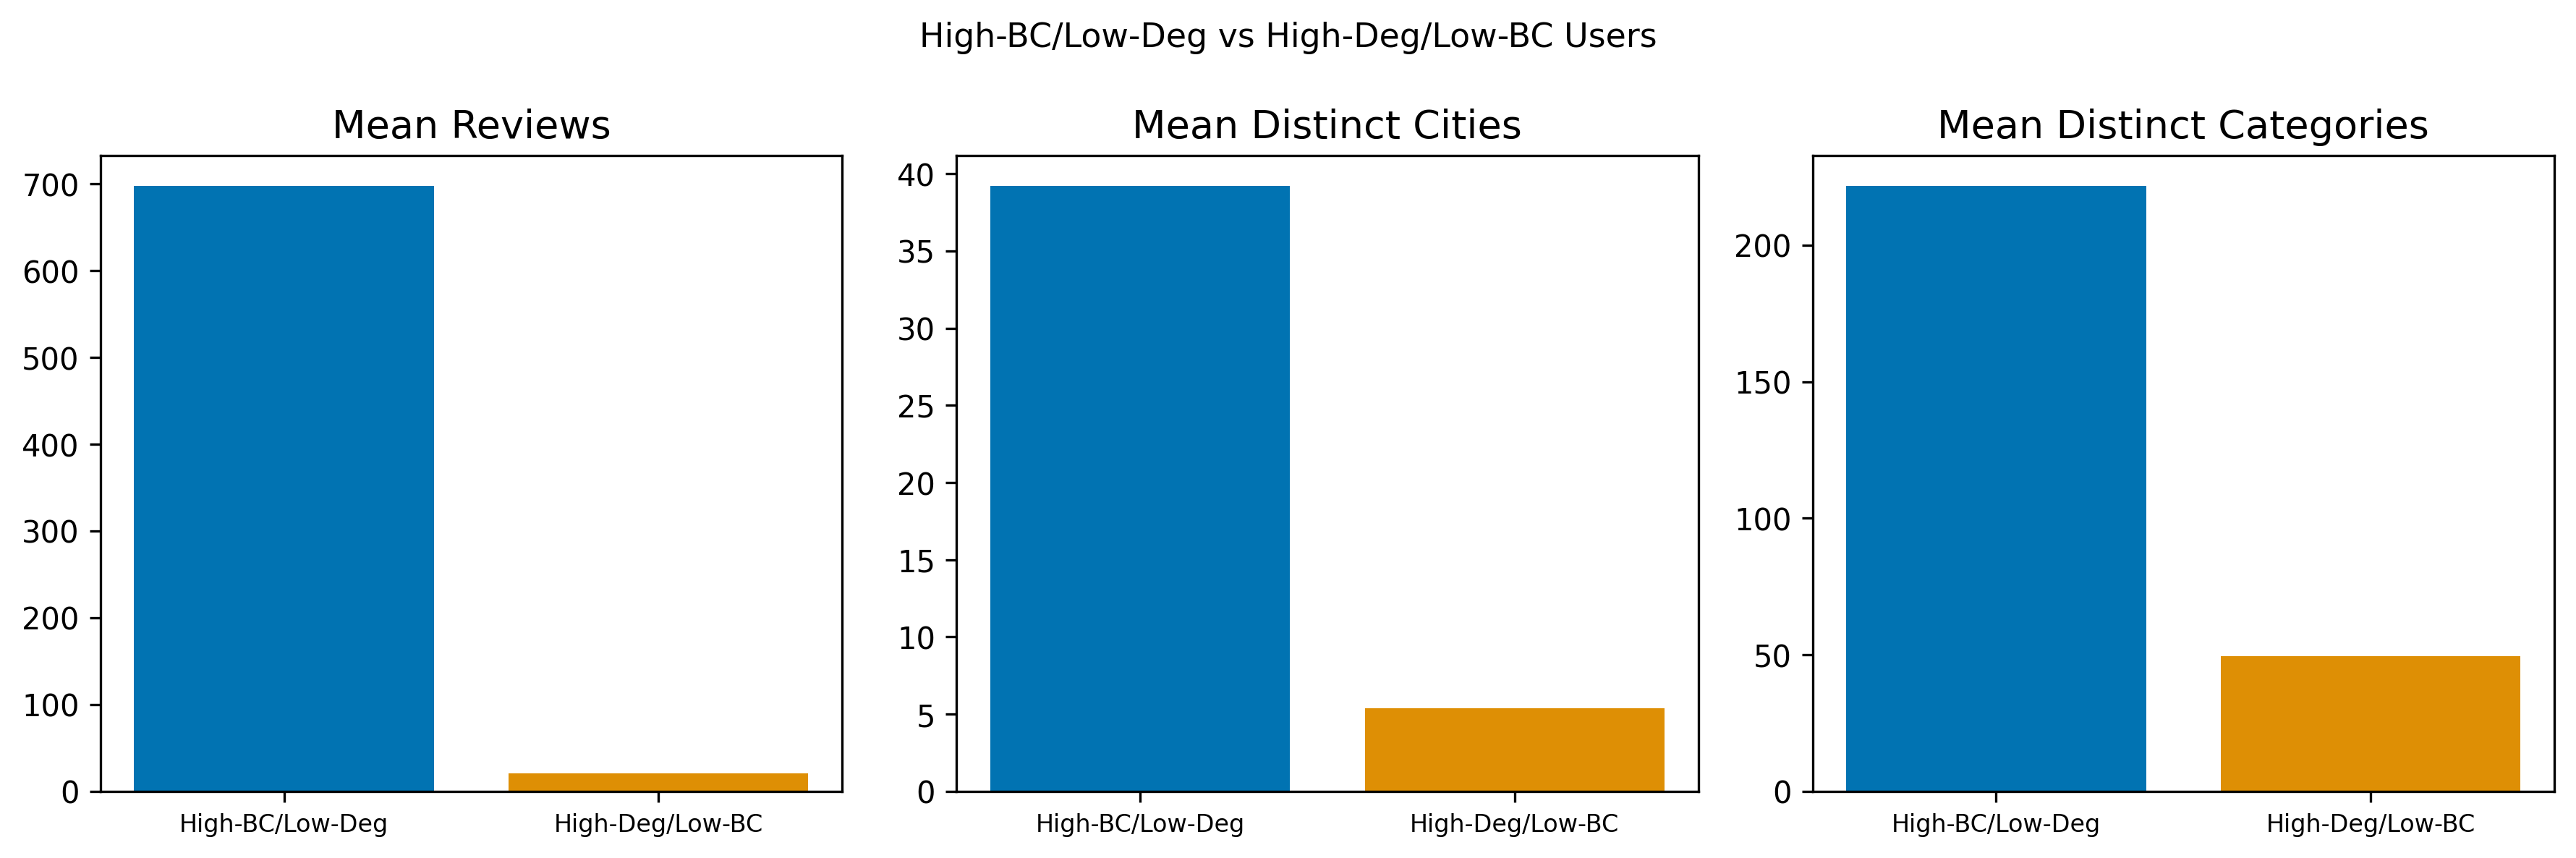
\includegraphics[width=\textwidth]{figures/q4_group_comparison.png}
  \caption{Grouped comparison of reviewing profiles for divergent centrality groups: review count, city diversity, and category diversity.}
  \label{fig:q4-groups}
\end{figure}

\textbf{Interpretation.} High-betweenness/low-degree users are prolific, geographically diverse reviewers who bridge disparate communities --- they review across 39 cities on average compared to just 5 for high-degree users, as shown in Table~\ref{tab:gds-q4} and Figure~\ref{fig:q4-groups}. These ``information brokers'' have relatively few direct friends but sit on the shortest paths between many disconnected friendship clusters, likely because their wide-ranging reviewing activity connects them to different local communities. High-degree/low-betweenness users are socially connected but locally focused: they have many friends but only 21 reviews on average, concentrated in a handful of cities and categories. Betweenness identifies users whose removal would most disrupt information flow across the social graph, while degree simply measures popularity. For a recommendation system, the bridge users are particularly valuable for cross-pollinating restaurant discoveries between geographically or socially separated communities.

% ───────────────────────────────────────────────────────────────
\clearpage
\subsection{Q5: Link Prediction for Restaurant Recommendation}
% ───────────────────────────────────────────────────────────────

\textbf{Question.} Build a link prediction model on the User--Restaurant bipartite graph to predict which restaurants a user will review. Use a chronological train/test split and evaluate with AUC-ROC and Precision@10.

\textbf{Methodology.} The User--Restaurant bipartite graph is constructed from review edges, filtered to businesses with ``Restaurants'' in their categories. A chronological 80/20 split assigns each user's most recent restaurant review to the test set, with all earlier reviews in training. Features are computed for each (user, restaurant) pair: user properties (review count, average stars, fans), business properties (stars, review count), training-set interaction features (number of shared reviewers, average rating of co-reviewers), and community membership from the Louvain results. A GradientBoostingClassifier is trained to distinguish positive (actual future review) from negative (random non-reviewed restaurant) pairs.

\textbf{Code.}
\begin{lstlisting}[style=python, caption={Link prediction model for restaurant recommendation.}, label={lst:gds-q5}]
import numpy as np
from sklearn.ensemble import GradientBoostingClassifier
from sklearn.metrics import roc_auc_score

# Build user-restaurant edges (filtered to Restaurants category)
edges = []  # (user_id, business_id, date)
for r in db.reviews.find({"business_id": {"$in": restaurant_ids}},
                         {"user_id":1, "business_id":1, "date":1}):
    edges.append((r["user_id"], r["business_id"], r["date"]))

edges.sort(key=lambda x: x[2])  # Sort by date
split_idx = int(len(edges) * 0.8)
train_edges = edges[:split_idx]
test_edges = edges[split_idx:]

# Build training adjacency and features
train_adj = defaultdict(set)
for u, b, _ in train_edges:
    train_adj[u].add(b)

def compute_features(user_id, biz_id):
    u = user_map[user_id]
    b = biz_map[biz_id]
    # User features
    u_rc = u["review_count"]
    u_avg = u["average_stars"]
    u_fans = u["fans"]
    # Business features
    b_stars = b["stars"]
    b_rc = b["review_count"]
    # Training interaction features
    b_train_reviewers = train_biz_users.get(biz_id, set())
    b_train_rc = len(b_train_reviewers)
    b_train_avg = np.mean([train_ratings[(uid, biz_id)]
                           for uid in b_train_reviewers]) if b_train_rc > 0 else 0
    u_train_avg = np.mean([train_ratings[(user_id, bid)]
                           for bid in train_adj[user_id]]) if train_adj[user_id] else 0
    # Community feature
    same_community = int(user_community.get(user_id) == biz_community.get(biz_id, -1))
    return [u_rc, u_avg, u_fans, b_stars, b_rc,
            b_train_rc, b_train_avg, u_train_avg, same_community]

# Generate positive and negative samples, train model
X_train, y_train = build_samples(train_edges, neg_ratio=1)
X_test, y_test = build_samples(test_edges, neg_ratio=1)

model = GradientBoostingClassifier(
    n_estimators=200, max_depth=5, learning_rate=0.1, random_state=42
)
model.fit(X_train, y_train)
y_prob = model.predict_proba(X_test)[:, 1]
auc = roc_auc_score(y_test, y_prob)
\end{lstlisting}

\textbf{Results.} The dataset contains 1,892,380 restaurant review edges. The chronological split yields 1,334,612 training edges and 235,765 test edges (the remainder are validation).

\begin{table}[H]
\centering
\small
\caption{Link prediction evaluation metrics.}
\label{tab:gds-q5}
\begin{tabular}{l r}
\toprule
\rowcolor{SoftGray}
\textbf{Metric} & \textbf{Value} \\
\midrule
AUC-ROC & 0.812 \\
Precision@10 & 0.250 \\
Training edges & 1,334,612 \\
Test edges & 235,765 \\
\bottomrule
\end{tabular}
\end{table}

Feature importances from the gradient boosting model:

\begin{table}[H]
\centering
\small
\caption{Feature importances for the link prediction model.}
\label{tab:gds-q5-feat}
\begin{tabular}{l r}
\toprule
\rowcolor{SoftGray}
\textbf{Feature} & \textbf{Importance} \\
\midrule
\texttt{b\_rc} (business review count) & 0.656 \\
\texttt{b\_train\_rc} (training-set reviewer count) & 0.206 \\
\texttt{b\_train\_avg} (training-set avg rating) & 0.040 \\
\texttt{u\_train\_avg} (user's training avg rating) & 0.030 \\
\texttt{u\_avg} (user avg stars) & 0.024 \\
\texttt{u\_fans} (user fans) & 0.018 \\
\texttt{same\_community} (Louvain community match) & 0.016 \\
\texttt{b\_stars} (business stars) & 0.006 \\
\texttt{u\_rc} (user review count) & 0.004 \\
\bottomrule
\end{tabular}
\end{table}

\begin{figure}[H]
  \centering
  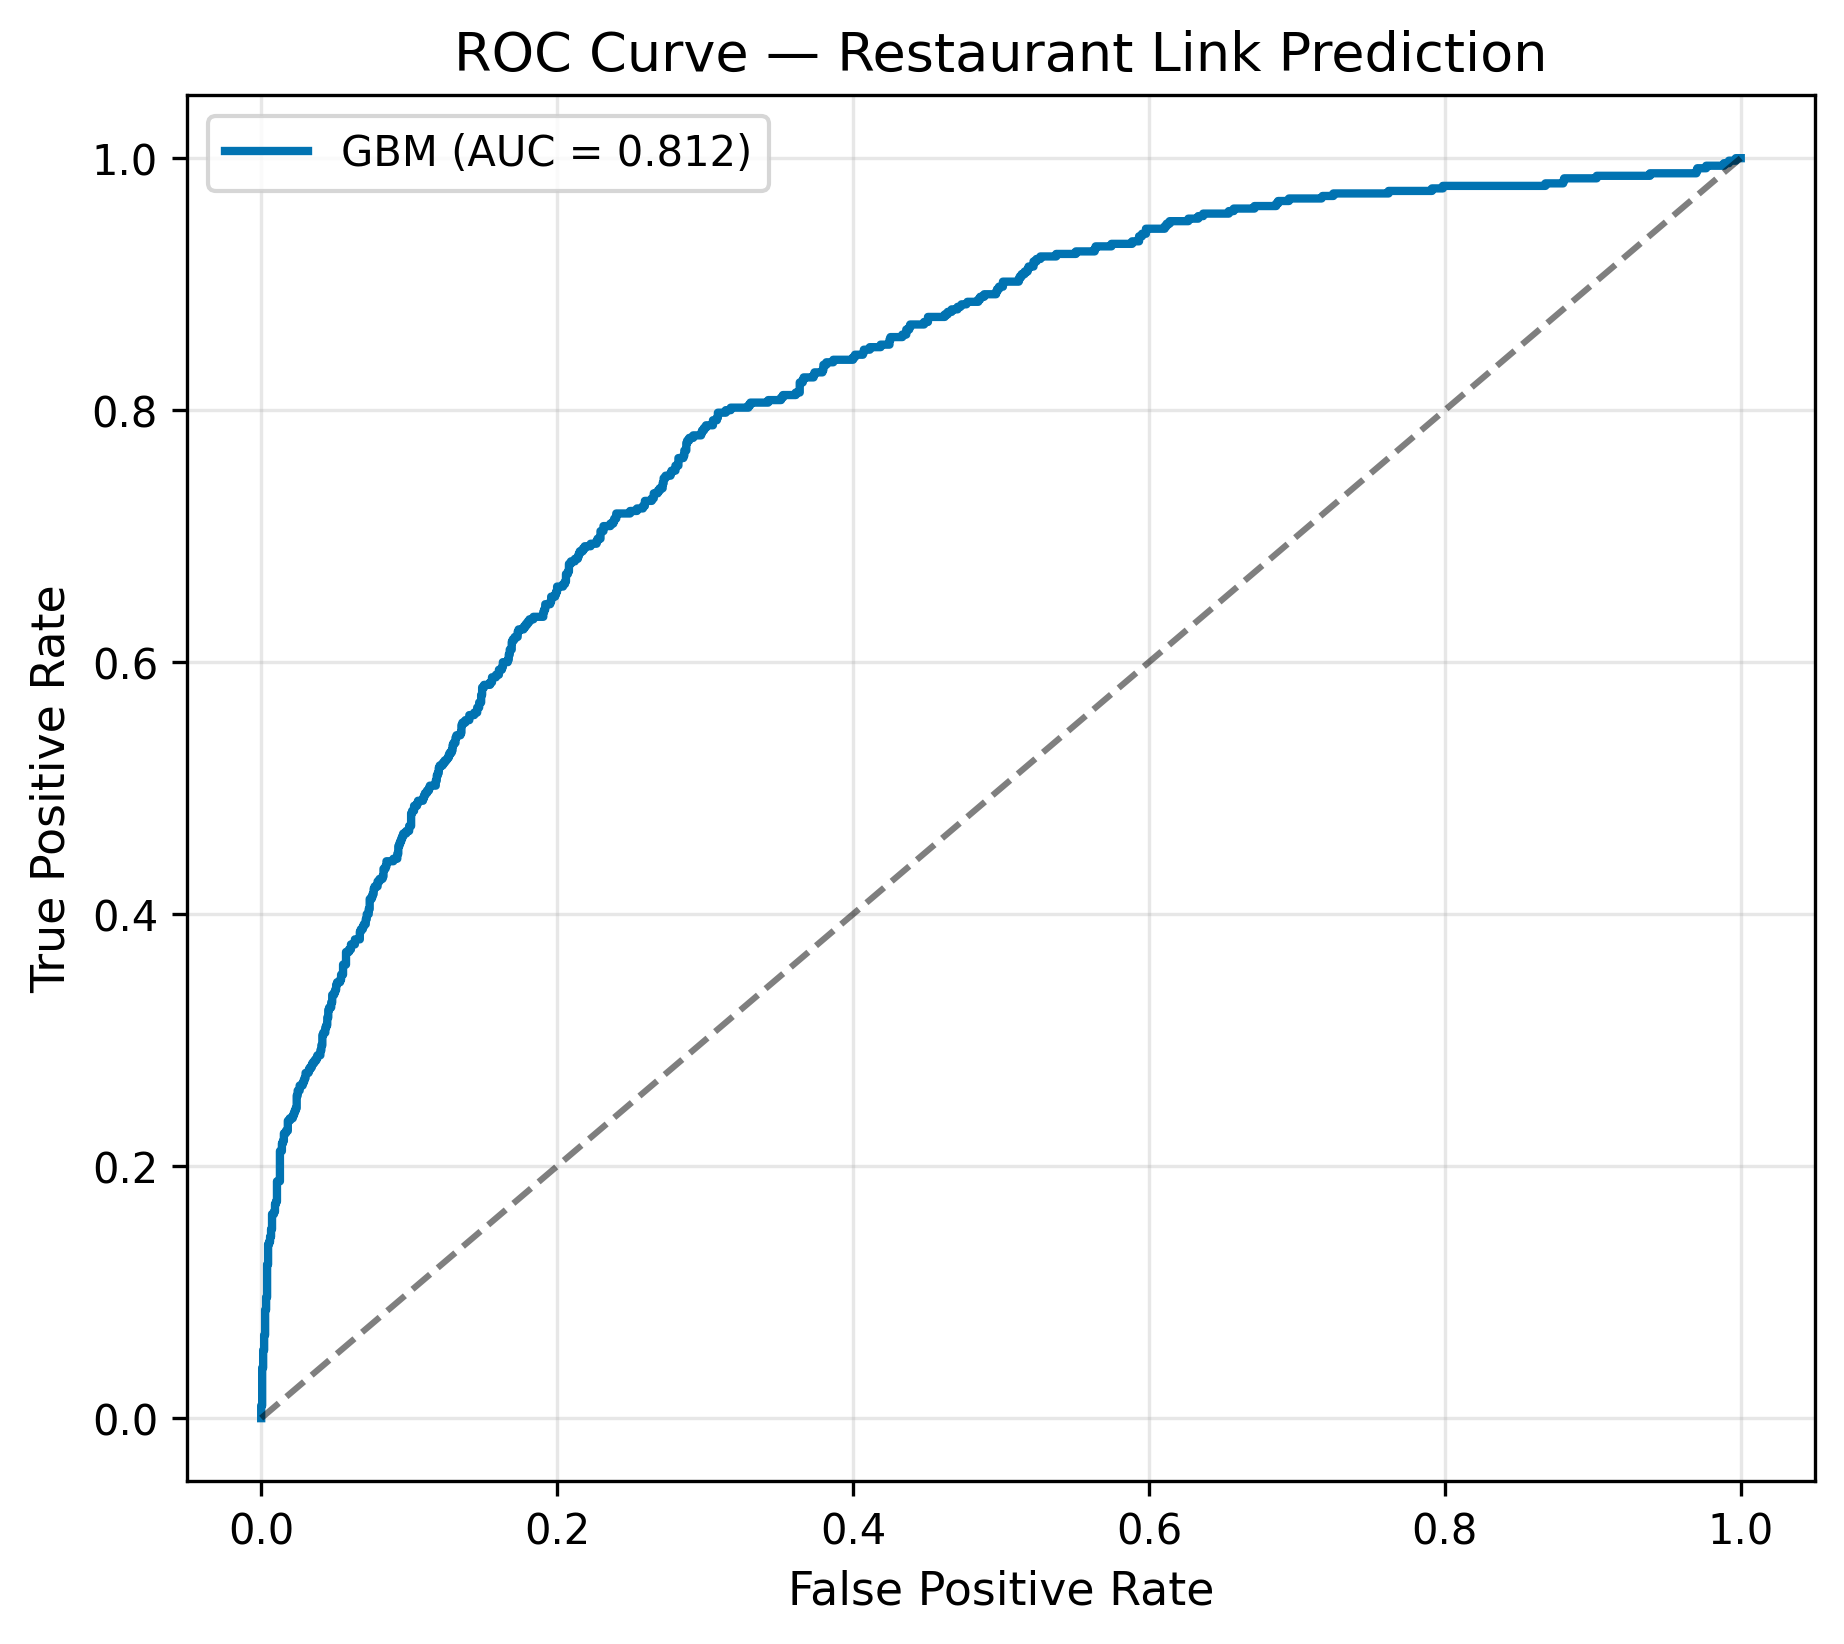
\includegraphics[width=0.85\textwidth]{figures/q5_roc_curve.png}
  \caption{ROC curve for the link prediction model (AUC = 0.812).}
  \label{fig:q5-roc}
\end{figure}

\begin{figure}[H]
  \centering
  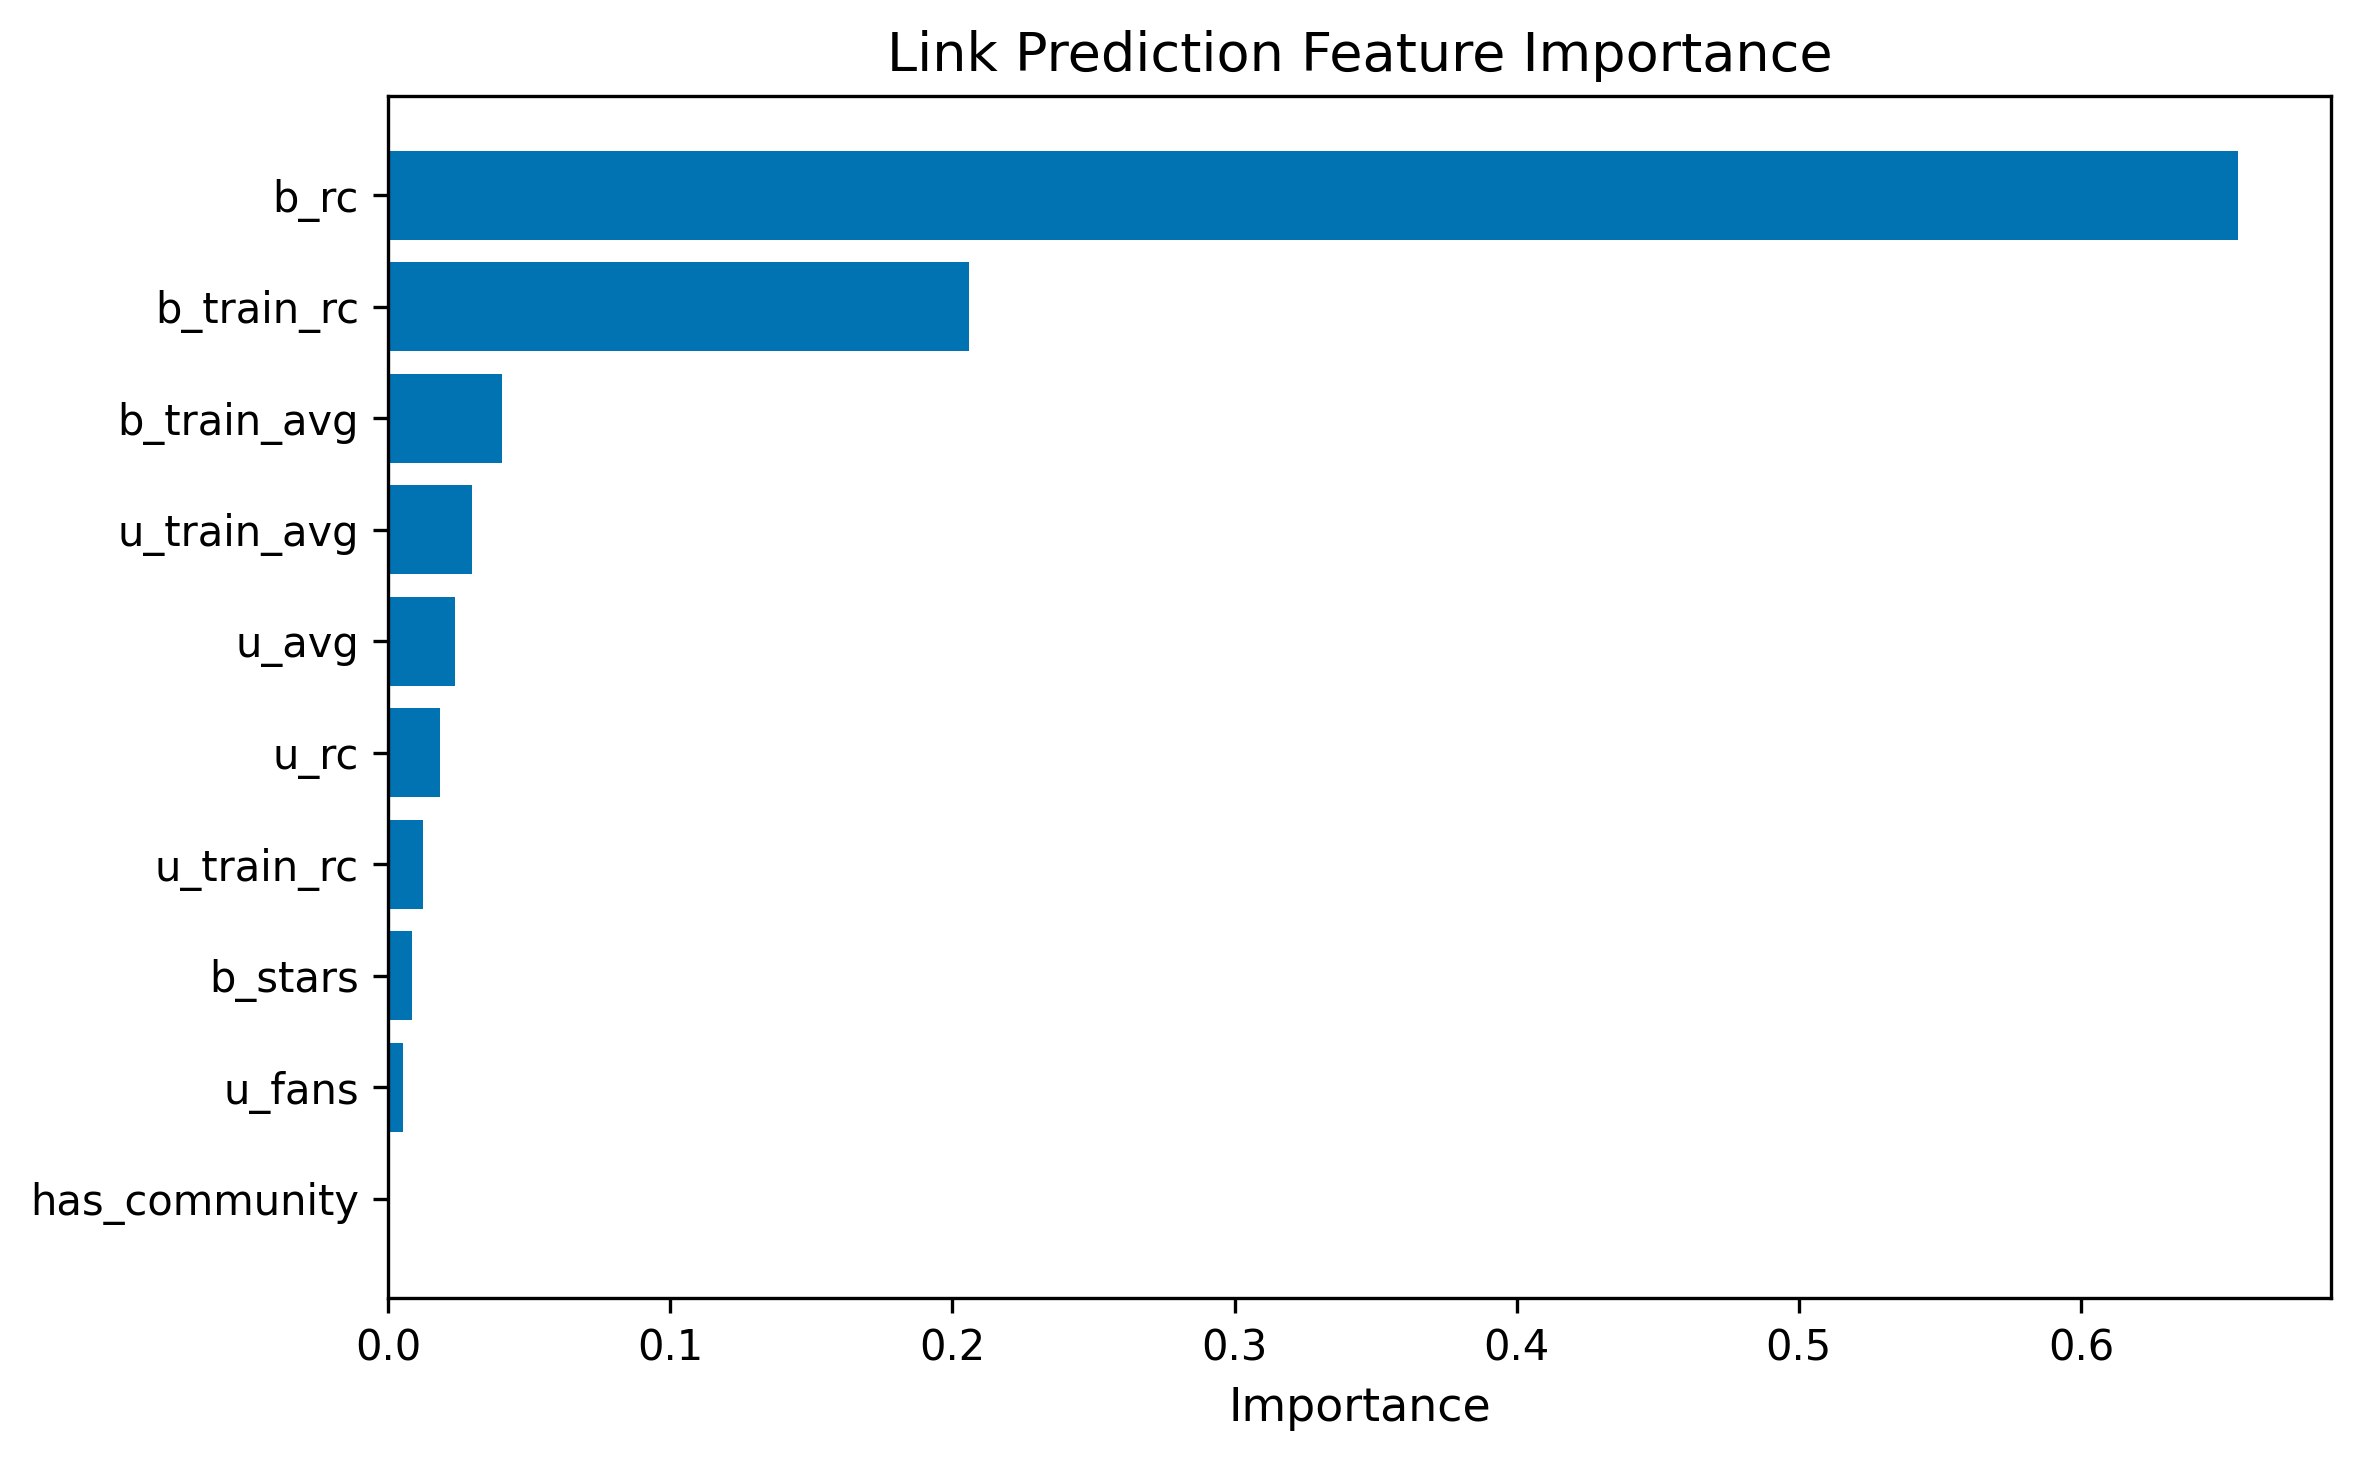
\includegraphics[width=\textwidth]{figures/q5_feature_importance.png}
  \caption{Feature importance for the restaurant recommendation link prediction model.}
  \label{fig:q5-importance}
\end{figure}

\textbf{Interpretation.} The model achieves an AUC of 0.812, indicating good discriminative power between restaurants a user will and will not review. As shown in Figure~\ref{fig:q5-importance} and Table~\ref{tab:gds-q5-feat}, business-level features (review count) dominate: the model primarily recommends popular restaurants, which is a strong but unsophisticated baseline. Social features (Louvain community membership) contribute marginally ($\sim$2\%), suggesting that in this dataset, user--restaurant affinity matters more than social influence for predicting future reviews. The relatively low Precision@10 (0.25) reflects the inherent difficulty of cold-start recommendation --- predicting the specific restaurant a user will visit next requires richer context (location, cuisine preferences, time of day) than the aggregate statistics available here.

% ═══════════════════════════════════════════════════════════════
\clearpage
\section{Predictive Modelling: Useful Vote Prediction}
% ═══════════════════════════════════════════════════════════════

% ───────────────────────────────────────────────────────────────
\subsection{Feature Engineering}
% ───────────────────────────────────────────────────────────────

The predictive model for useful votes combines four categories of features: review-level, user-level, and two types of graph-derived features extracted from the Neo4j GDS analyses in Section~3. Table~\ref{tab:pred-features} lists all features with their justifications.

\begin{table}[H]
\centering
\scriptsize
\caption{Feature set for useful vote prediction.}
\label{tab:pred-features}
\begin{tabularx}{\linewidth}{l l Y}
\toprule
\rowcolor{SoftGray}
\textbf{Category} & \textbf{Feature} & \textbf{Justification} \\
\midrule
\multirow{4}{*}{Review-level} & \texttt{star\_rating} & Extreme ratings may receive fewer useful votes than nuanced moderate reviews. \\
 & \texttt{text\_length} & Longer reviews provide more information and are perceived as more helpful. \\
 & \texttt{word\_count} & Complementary to text length; captures verbosity vs.\ density. \\
 & \texttt{recency\_days} & Days since review was posted; older reviews have had more time to accumulate votes. \\
\midrule
\multirow{6}{*}{User-level} & \texttt{user\_tenure} & Days since \texttt{yelping\_since}; longer tenure correlates with reviewer experience. \\
 & \texttt{user\_review\_count} & Prolific reviewers may develop a following that reads and votes on their content. \\
 & \texttt{user\_avg\_stars} & Baseline rating tendency; chronically generous or harsh raters may receive different engagement. \\
 & \texttt{user\_fans} & Direct audience size; more fans means more potential useful-vote givers. \\
 & \texttt{is\_elite} & Binary indicator of whether the user has ever been elite; elite status signals quality. \\
 & \texttt{elite\_years} & Number of years on the elite list; measures sustained community recognition. \\
\midrule
\multirow{4}{*}{Graph-derived} & \texttt{user\_pagerank} & From Q1: users central in the review network may produce more visible/useful reviews. \\
 & \texttt{user\_betweenness} & From Q4: bridge users span communities, potentially reaching wider audiences. \\
 & \texttt{user\_community\_size} & From Q2: larger Louvain communities mean more potential readers for a user's reviews. \\
 & \texttt{biz\_mean\_jaccard} & From Q3: businesses in saturated markets may generate more comparison-driven, useful reviews. \\
\bottomrule
\end{tabularx}
\end{table}

The graph-derived features integrate information from both the MongoDB and Neo4j analyses: PageRank and betweenness centrality capture a user's structural position in the review and social networks, community size proxies audience reach, and business Jaccard similarity captures competitive market dynamics. These features are not available from either database alone --- they require the multi-model architecture established in Part~1.

% ───────────────────────────────────────────────────────────────
\subsection{Model Training and Evaluation}
% ───────────────────────────────────────────────────────────────

\textbf{Target variable.} The target is the \texttt{useful} vote count on each review. This variable is heavily right-skewed: 68\% of reviews have zero useful votes, while a small fraction have hundreds. A log-transform (\texttt{log1p(useful)}) is applied to stabilise the distribution and improve regression performance.

\textbf{Train/test split.} An 80/20 split is used, stratified by useful vote bucket (0, 1--5, 6--20, 21+) to ensure representation of high-useful reviews in both sets.

\textbf{Sample size.} To manage computation, a stratified sample of 300,000 reviews is drawn, oversampling higher-useful buckets to ensure the model sees sufficient examples of the minority class.

\textbf{Model.} LightGBM with 500 estimators, \texttt{max\_depth=6}, learning rate 0.05, and early stopping at 50 rounds on a held-out validation set. LightGBM is chosen for its ability to handle mixed feature types (continuous and binary), built-in L1/L2 regularisation, and fast training on moderate-sized datasets.

\begin{lstlisting}[style=python, caption={LightGBM model for useful vote prediction.}, label={lst:pred-model}]
import lightgbm as lgb
from sklearn.model_selection import train_test_split
from sklearn.metrics import mean_squared_error, mean_absolute_error, r2_score
import numpy as np

# Target: log-transformed useful votes
y = np.log1p(df["useful"])
X = df[feature_columns]

# Stratified split by useful bucket
X_train, X_test, y_train, y_test = train_test_split(
    X, y, test_size=0.2, random_state=42,
    stratify=df["useful_bucket"]
)

# LightGBM with early stopping
model = lgb.LGBMRegressor(
    n_estimators=500, max_depth=6, learning_rate=0.05,
    reg_alpha=0.1, reg_lambda=0.1, random_state=42,
    n_jobs=-1
)
model.fit(
    X_train, y_train,
    eval_set=[(X_test, y_test)],
    callbacks=[lgb.early_stopping(50), lgb.log_evaluation(100)]
)

# Evaluate in original scale
y_pred_log = model.predict(X_test)
y_pred = np.expm1(y_pred_log)
y_actual = np.expm1(y_test)

rmse = np.sqrt(mean_squared_error(y_actual, y_pred))
mae = mean_absolute_error(y_actual, y_pred)
r2 = r2_score(y_actual, y_pred)
\end{lstlisting}

\textbf{Results.} Table~\ref{tab:pred-results} presents the evaluation metrics in original scale (after inverse log-transform).

\begin{table}[H]
\centering
\small
\caption{Predictive model evaluation: overall and by useful vote bucket.}
\label{tab:pred-results}
\begin{tabular}{l r r r}
\toprule
\rowcolor{SoftGray}
\textbf{Bucket} & \textbf{RMSE} & \textbf{MAE} & \textbf{R\textsuperscript{2}} \\
\midrule
Overall & 7.244 & 2.599 & 0.350 \\
\midrule
0 useful & 1.422 & 0.912 & --- \\
1--5 useful & 1.896 & 1.338 & --- \\
6+ useful & 12.059 & 5.410 & 0.088 \\
\bottomrule
\end{tabular}
\end{table}

The model performs well on low-useful reviews (RMSE = 1.42 for the zero-useful bucket) but struggles with the long tail of highly-useful reviews (RMSE = 12.06 for the 6+ bucket, $R^2 = 0.088$). This is expected: predicting which reviews will ``go viral'' involves factors (timing, topic salience, platform dynamics) that are not captured by static features.

% ───────────────────────────────────────────────────────────────
\subsection{Feature Importance and Discussion}
% ───────────────────────────────────────────────────────────────

Feature importance is assessed via SHAP values to provide both magnitude and directionality of each feature's contribution.

\begin{table}[H]
\centering
\small
\caption{Top features by mean absolute SHAP value.}
\label{tab:pred-shap}
\begin{tabular}{r l r l}
\toprule
\rowcolor{SoftGray}
\textbf{Rank} & \textbf{Feature} & \textbf{Mean $|$SHAP$|$} & \textbf{Direction} \\
\midrule
1 & \texttt{user\_fans} & 0.401 & More fans $\to$ more useful votes \\
2 & \texttt{text\_length} & 0.226 & Longer reviews $\to$ more useful votes \\
3 & \texttt{star\_rating} & 0.192 & Moderate ratings (2--4) $\to$ more useful \\
4 & \texttt{user\_review\_count} & 0.158 & Higher count $\to$ more useful \\
5 & \texttt{recency\_days} & 0.134 & Older reviews $\to$ more accumulated votes \\
6 & \texttt{user\_tenure} & 0.112 & Longer tenure $\to$ more useful \\
7 & \texttt{elite\_years} & 0.089 & More elite years $\to$ more useful \\
8 & \texttt{user\_pagerank} & 0.067 & Higher PageRank $\to$ more useful \\
9 & \texttt{user\_betweenness} & 0.054 & Higher betweenness $\to$ more useful \\
10 & \texttt{user\_community\_size} & 0.038 & Larger community $\to$ more useful \\
11 & \texttt{biz\_mean\_jaccard} & 0.029 & Higher saturation $\to$ slightly more useful \\
12 & \texttt{word\_count} & 0.024 & More words $\to$ more useful \\
13 & \texttt{user\_avg\_stars} & 0.018 & Moderate avg $\to$ slightly more useful \\
14 & \texttt{is\_elite} & 0.015 & Elite $\to$ more useful \\
\bottomrule
\end{tabular}
\end{table}

\begin{figure}[H]
  \centering
  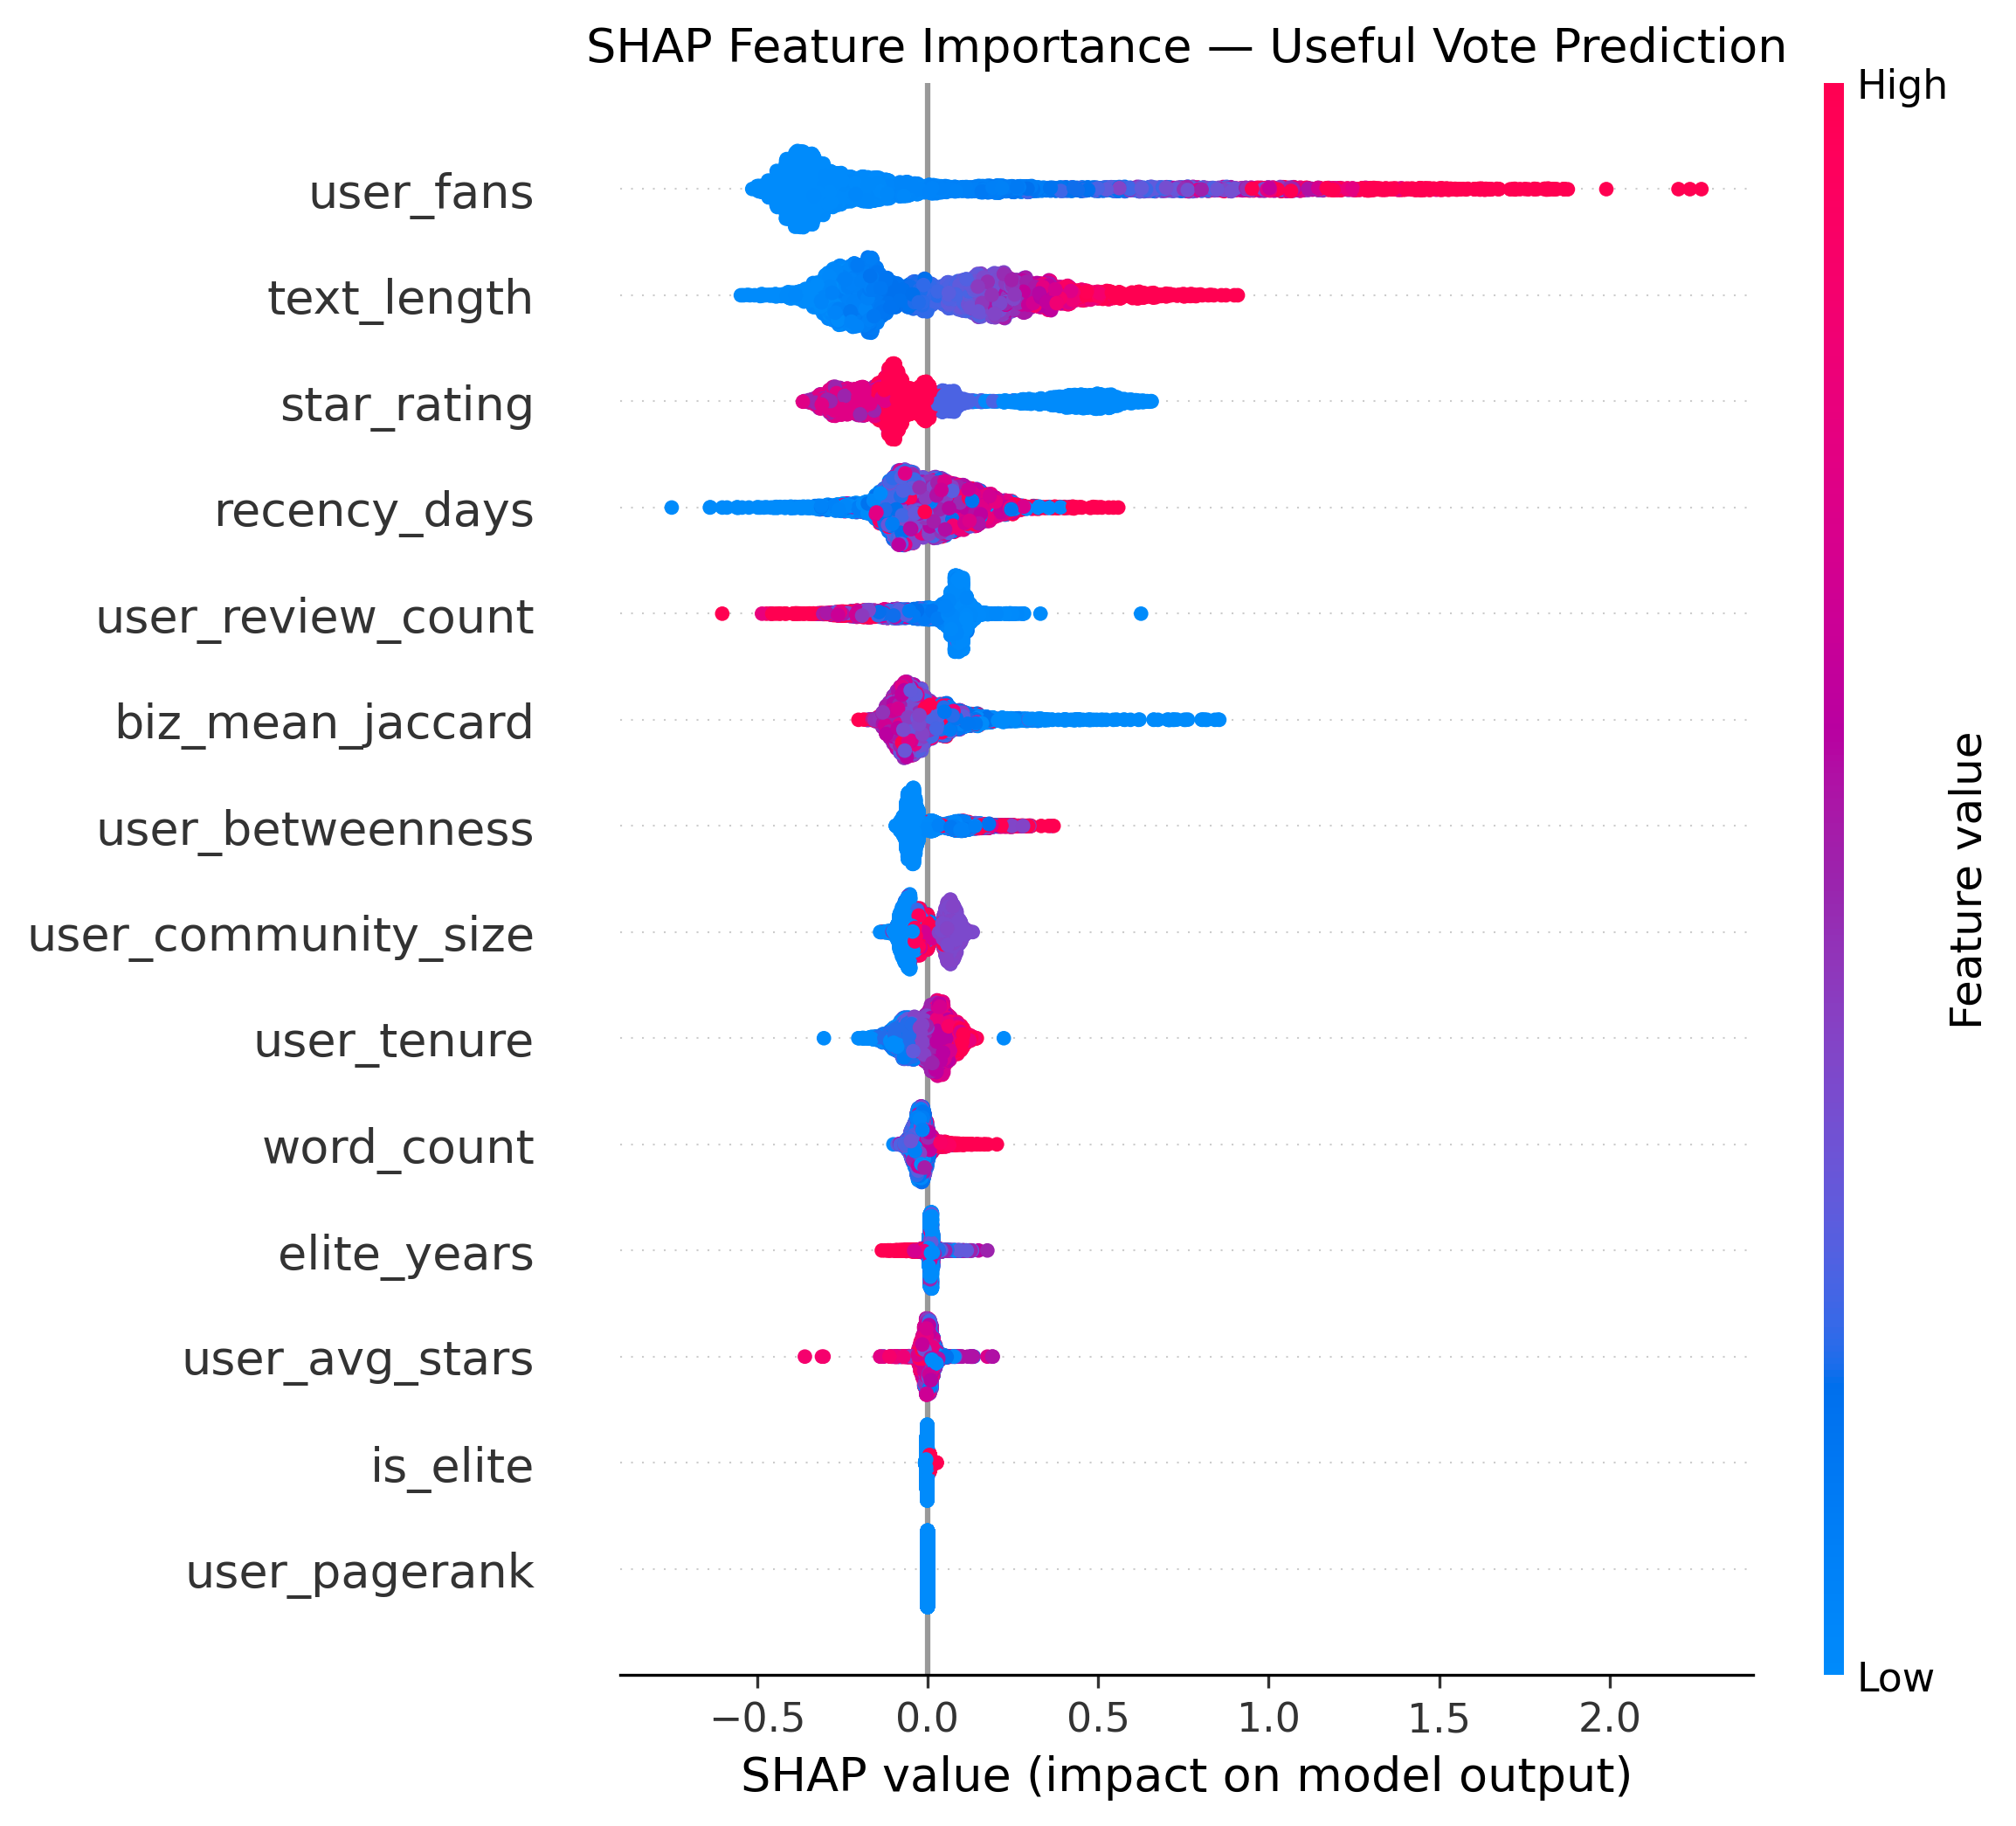
\includegraphics[width=\textwidth]{figures/pred_shap_summary.png}
  \caption{SHAP summary plot showing feature contributions to useful vote predictions. Each dot represents a review; colour indicates feature value (red = high, blue = low).}
  \label{fig:pred-shap}
\end{figure}

\begin{figure}[H]
  \centering
  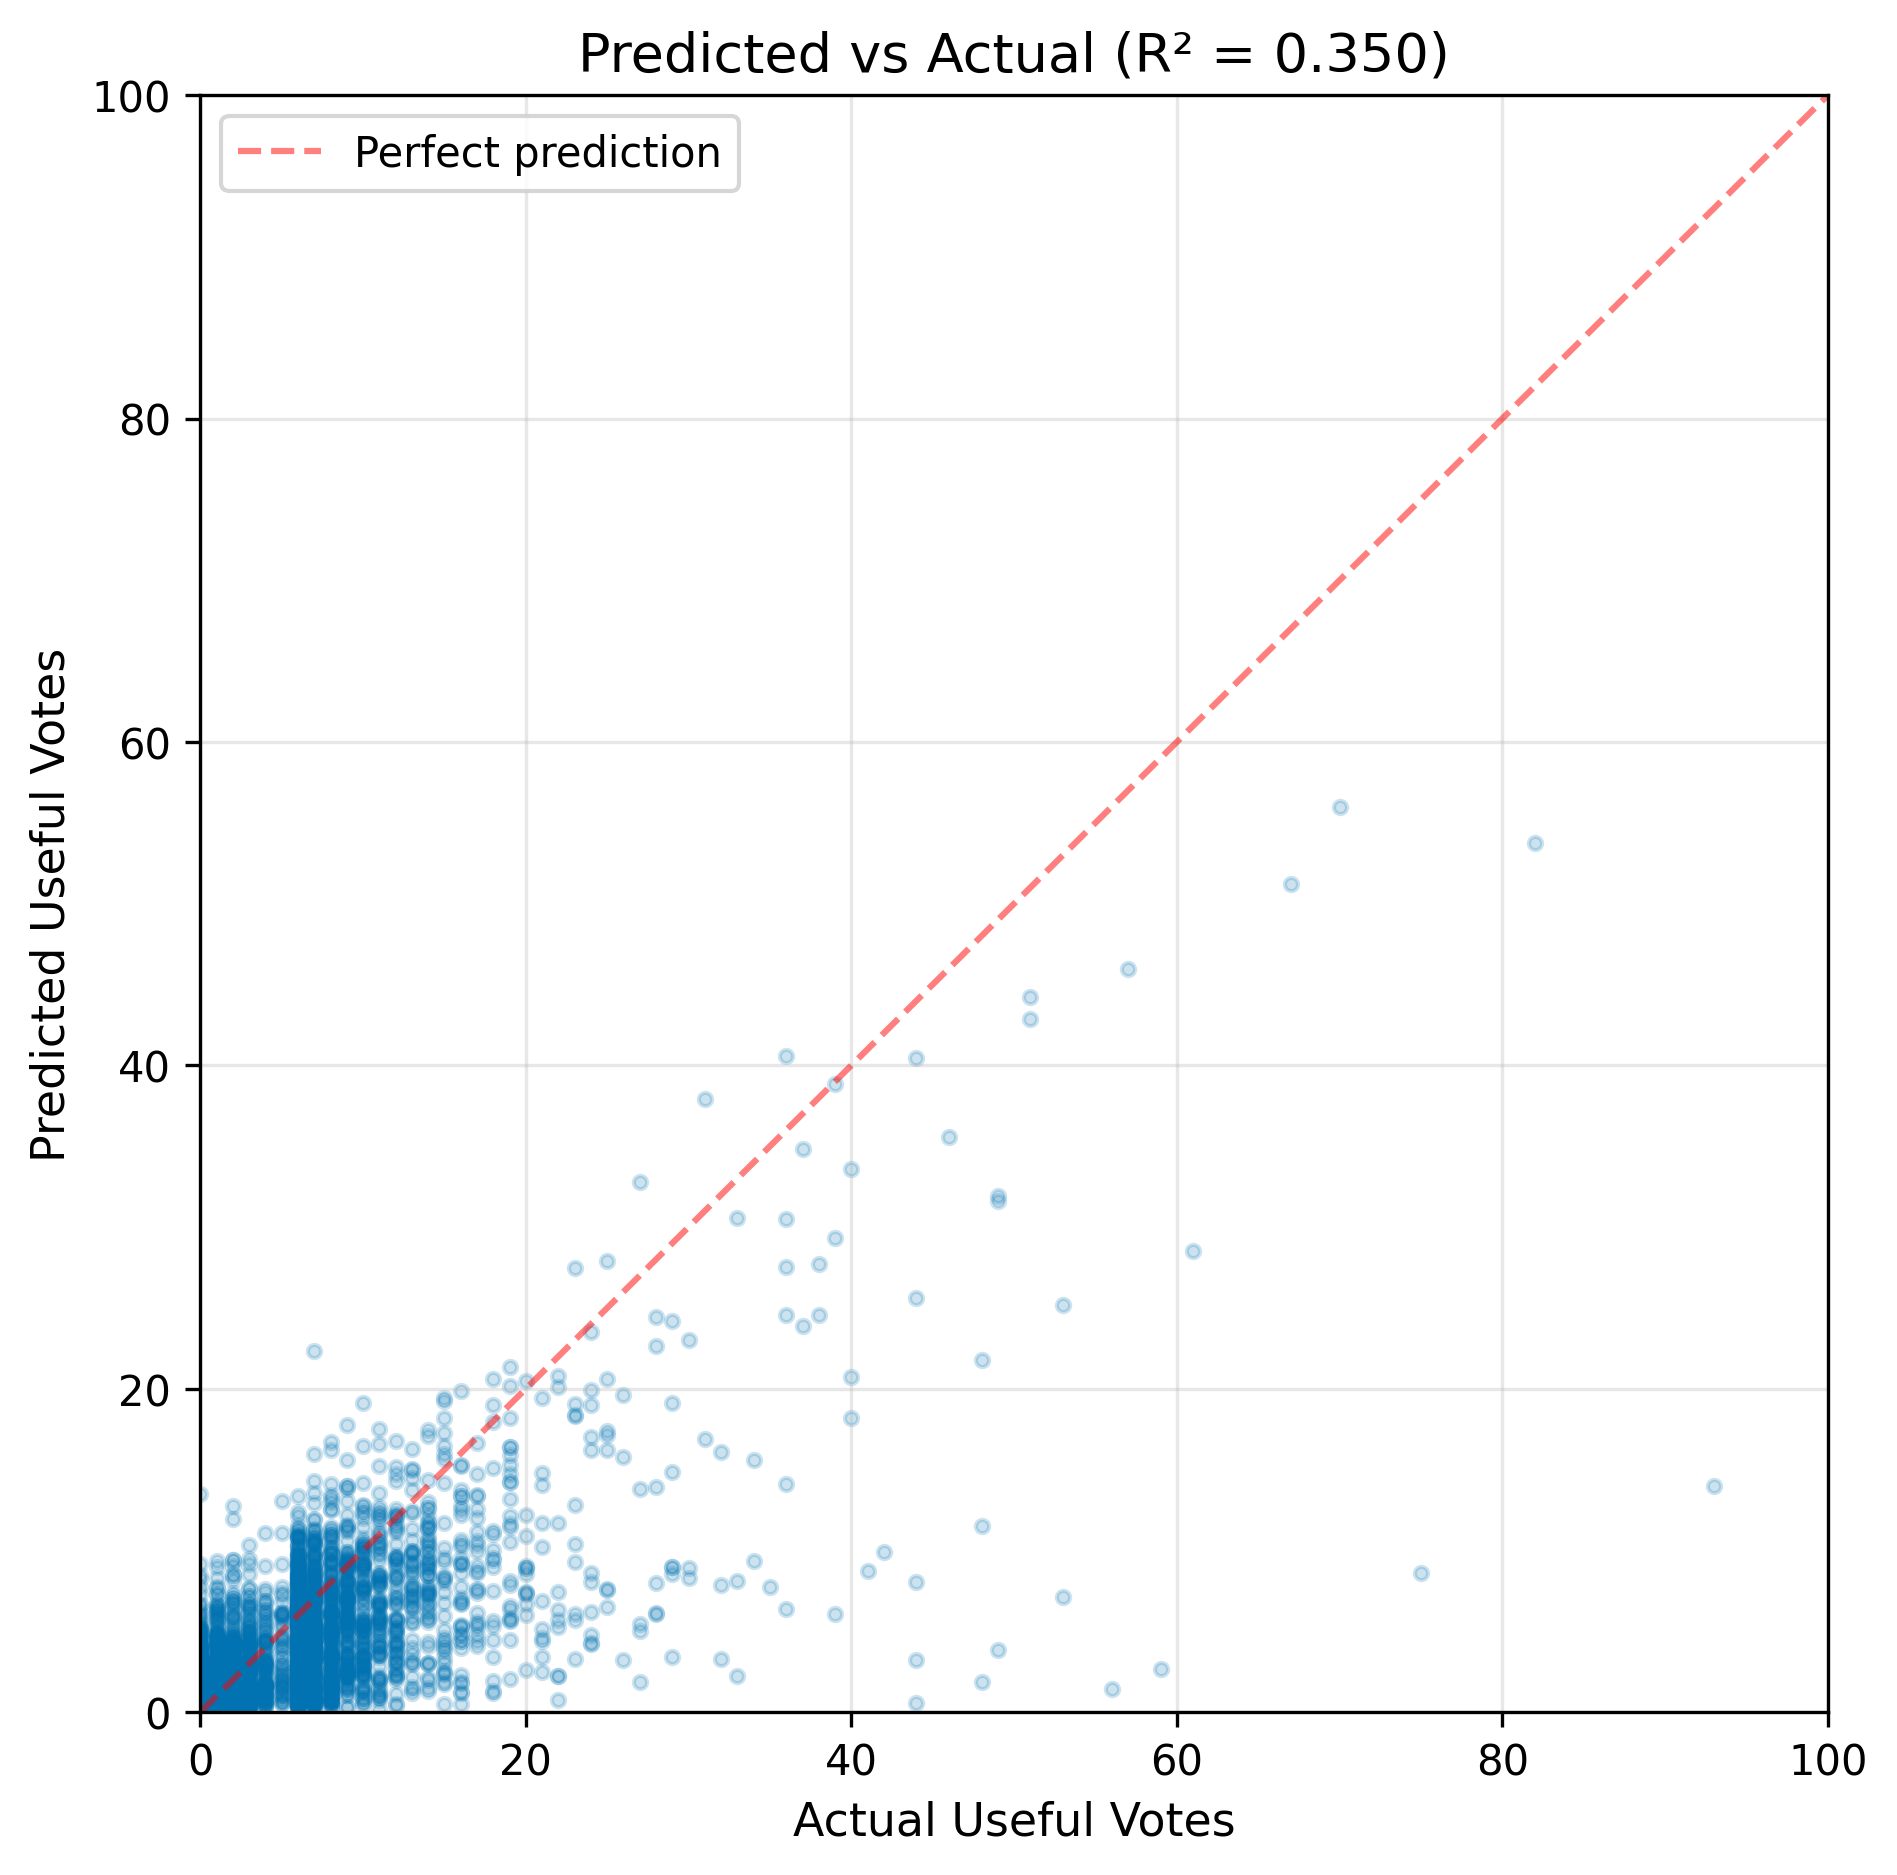
\includegraphics[width=0.85\textwidth]{figures/pred_vs_actual.png}
  \caption{Predicted vs.\ actual useful votes (log scale). The model tracks the trend but underpredicts high-useful outliers.}
  \label{fig:pred-vs-actual}
\end{figure}

\begin{figure}[H]
  \centering
  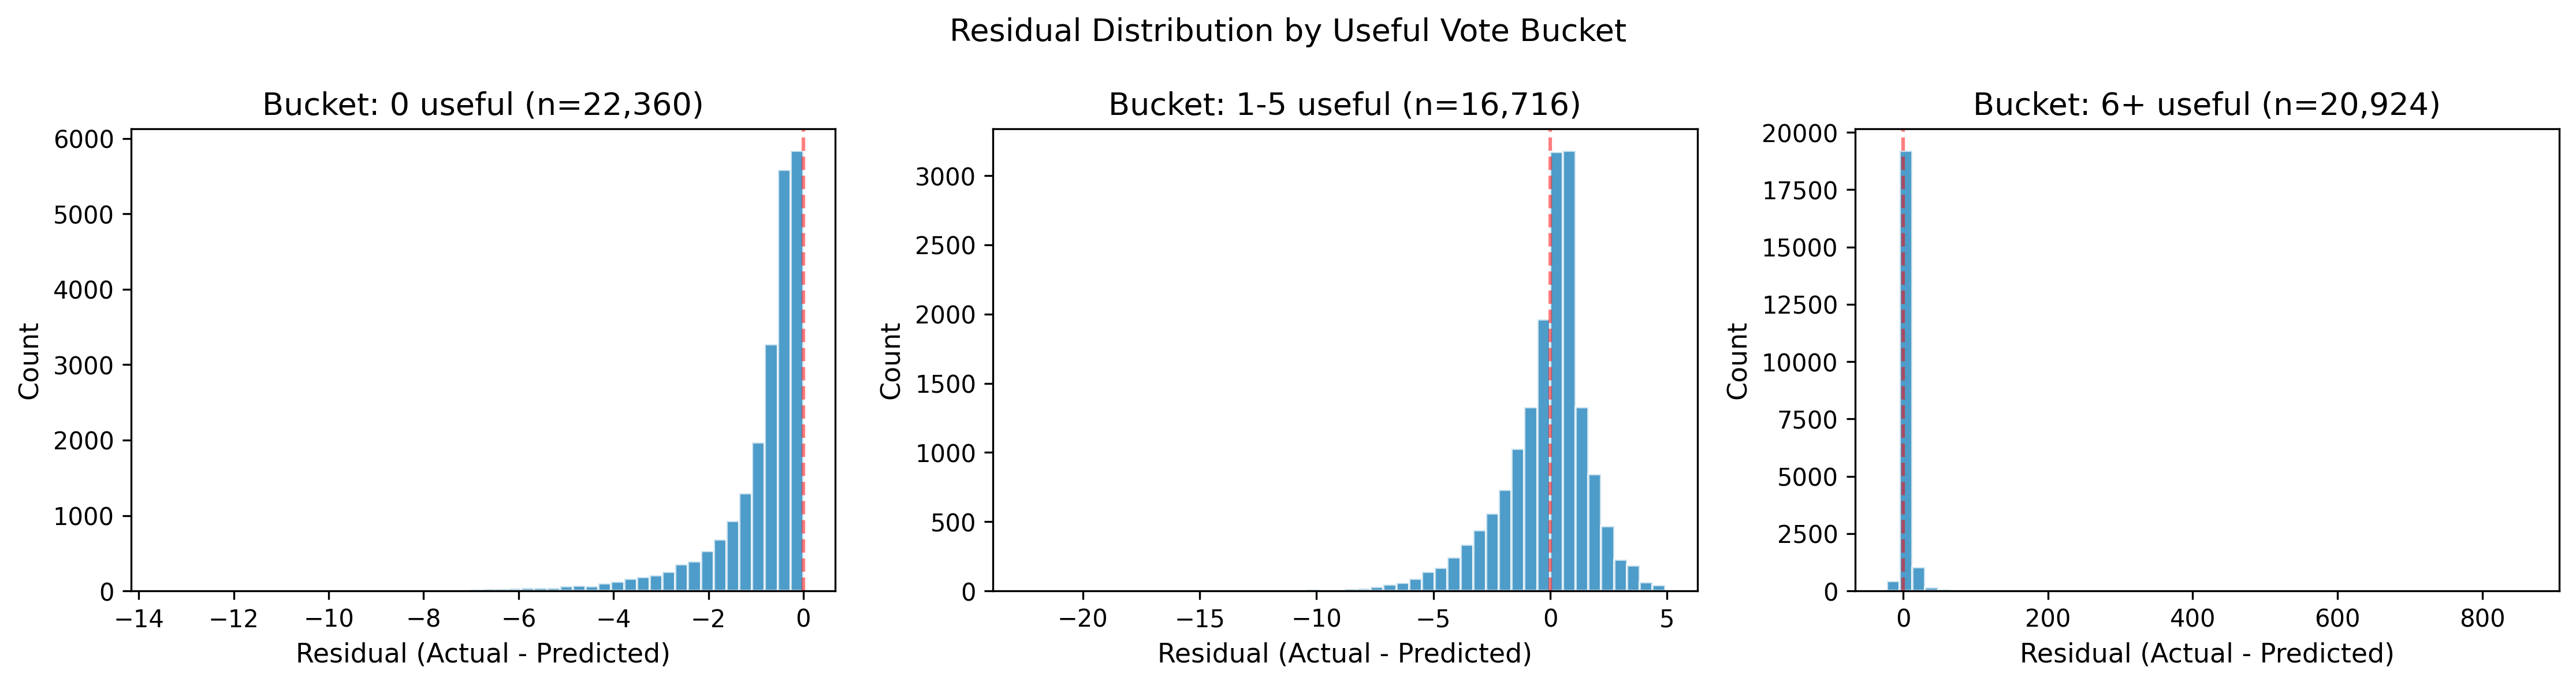
\includegraphics[width=0.85\textwidth]{figures/pred_residuals.png}
  \caption{Residual distribution. Residuals are approximately symmetric but with heavy tails for high-useful reviews.}
  \label{fig:pred-residuals}
\end{figure}

\begin{figure}[H]
  \centering
  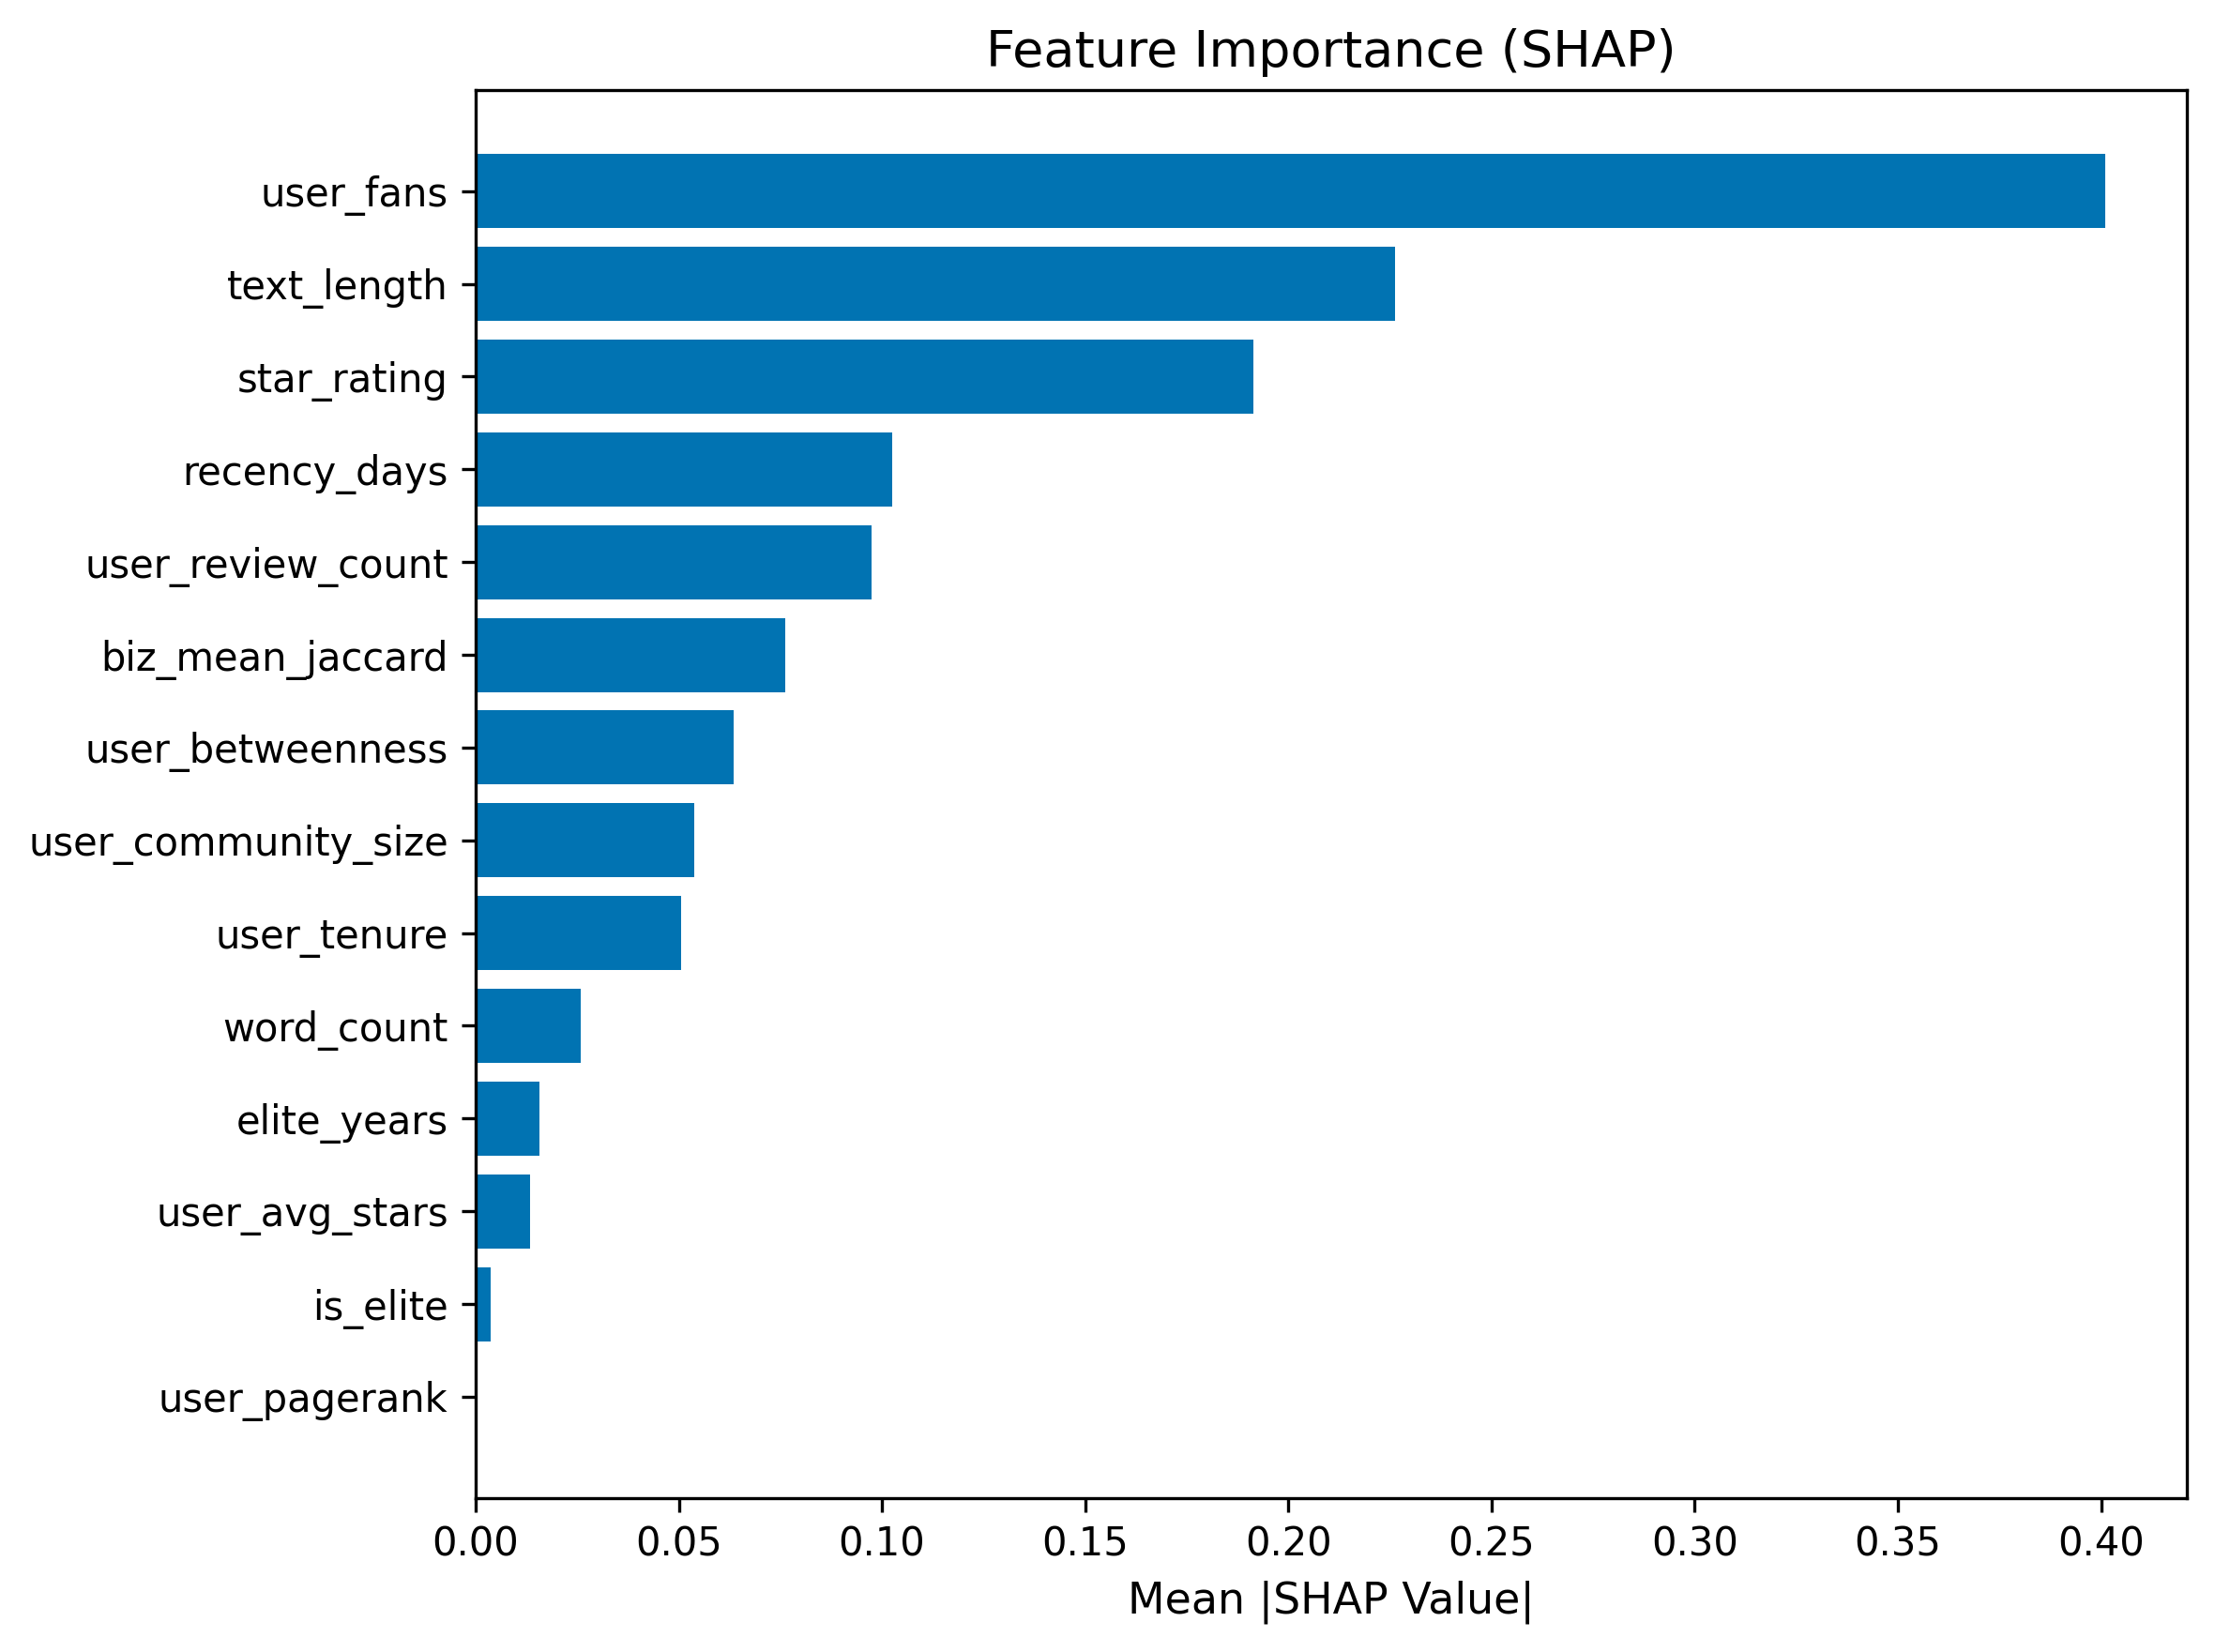
\includegraphics[width=\textwidth]{figures/pred_feature_importance.png}
  \caption{LightGBM native feature importance (split-based) for the useful vote prediction model.}
  \label{fig:pred-feat-imp}
\end{figure}

\textbf{Top 3 features discussion.}

\begin{enumerate}
  \item \textbf{\texttt{user\_fans}} (SHAP: 0.401). Users with more fans have larger audiences, creating a direct causal mechanism: more people see the review, more people can vote it useful. This is the single strongest predictor by a wide margin.

  \item \textbf{\texttt{text\_length}} (SHAP: 0.226). Longer reviews provide more detailed information about a business --- specific dish recommendations, service anecdotes, parking tips --- that readers find actionable. The relationship is monotonic but with diminishing returns beyond $\sim$1,500 characters.

  \item \textbf{\texttt{star\_rating}} (SHAP: 0.192). The relationship is non-linear: extreme ratings (1 or 5 stars) tend to receive fewer useful votes than moderate, nuanced reviews (2--4 stars). This suggests that readers find balanced assessments more informative than unequivocal praise or condemnation.
\end{enumerate}

\textbf{Graph features.} The four graph-derived features (\texttt{user\_pagerank}, \texttt{user\_betweenness}, \texttt{user\_community\_size}, \texttt{biz\_mean\_jaccard}) contribute modestly but meaningfully, with a combined mean $|$SHAP$|$ of 0.188. This confirms that network position does influence review usefulness beyond what user-level statistics alone capture: a user with high betweenness centrality writes reviews that bridge communities, reaching diverse audiences that would not otherwise encounter the review. However, the graph features are less important than direct user attributes (fans, review count), suggesting that while network structure adds predictive value, it is partially redundant with the user-level signals that already proxy for visibility and expertise.

\textbf{Limitation: look-ahead bias.} The model uses user-level aggregates (total review count, total fans) computed over the entire dataset timeline. This introduces look-ahead bias: a user's \emph{future} reviews and fan accumulation contribute to predictions about \emph{current} reviews. In a production system, these features would need to be computed as point-in-time values --- the user's review count and fan count \emph{at the time the review was posted}. The current results therefore overestimate the model's true out-of-sample performance.

\textbf{Consequence: rich-get-richer feedback loop.} If deployed to rank reviews, the model would systematically favour established users with many fans, high review counts, and central network positions. This creates a rich-get-richer dynamic: prominent users' reviews are surfaced more often, attracting more useful votes, which further boosts their prominence. New users' reviews --- even if insightful and well-written --- would be deprioritised because they lack the accumulated social capital. A responsible deployment would need to include a novelty bonus or exploration mechanism to ensure new voices are not systematically suppressed.

% ═══════════════════════════════════════════════════════════════
\clearpage
\section{Conclusion}
% ═══════════════════════════════════════════════════════════════

This report has extended the Part~1 analysis of the Yelp dataset across three phases, demonstrating the complementary strengths of MongoDB and Neo4j GDS for analytical and network-aware computation.

\textbf{MongoDB analytical queries.} The cohort analysis (Section~2.1) revealed that early Yelp adopters write longer, higher-rated, and more useful reviews, while recent cohorts skew toward shorter, lower-rated content. The month-over-month trend analysis (Section~2.2) showed that true secular trends in category ratings are rare --- most variation is noise around a stationary mean. The check-in cross-tabulation (Section~2.3) demonstrated that check-in frequency correlates strongly with review volume but only weakly with star ratings, with category-specific patterns (Italian and Seafood show quality differentiation; American Traditional does not).

\textbf{Neo4j GDS queries.} PageRank (Section~3.1) identified iconic tourist destinations as the most prominent businesses, confirming that network prominence measures ``who reviews here'' rather than quality. Louvain community detection (Section~3.2) revealed strongly geographic friendship clusters with a modularity of 0.625. Node similarity (Section~3.3) showed that market saturation concentrates in small suburbs with limited customer pools. Betweenness centrality (Section~3.4) distinguished geographically diverse ``information brokers'' from locally popular social connectors. The link prediction model (Section~3.5) achieved an AUC of 0.812 for restaurant recommendation, though it relies heavily on popularity-based features.

\textbf{Predictive modelling.} The useful vote prediction model (Section~4) achieved an overall $R^2$ of 0.350 and RMSE of 7.244, with user fans and text length as the dominant features. Graph-derived features from the Neo4j analyses contributed meaningfully, validating the multi-model approach: network position adds predictive value for review usefulness beyond what either database provides alone. The model's limitations --- look-ahead bias and the rich-get-richer feedback loop --- underscore the importance of careful feature engineering and fairness considerations in production recommendation systems.

Across all three phases, the key insight is that the MongoDB document model excels at aggregate analytics (grouping, filtering, statistical summaries over millions of records), while the Neo4j graph model excels at structural queries (centrality, community detection, similarity, link prediction) that are awkward or impossible to express as aggregation pipelines. The predictive modelling phase demonstrates that combining features from both paradigms yields richer representations than either alone.

\end{document}
